\documentclass[11pt,letterpaper]{article}
\usepackage{jahnel}
\usepackage{graphicx}
\DeclareMathOperator{\dist}{dist}
\newcommand{\cS}{\mathcal S}
\newcommand{\cW}{\mathcal W}
\newcommand{\cC}{\mathcal C}

\runningtitle{Isotropic Poisson line Cox percolation}
\hypersetup{pdftitle={A nontrivial phase transition for isotropic Poisson line Cox percolation},pdfauthor={Christian Hirsch, Benedikt Jahnel}}

\title{\textbf{A nontrivial phase transition for isotropic\\ Poisson line Cox percolation}}

\author{%
  Christian Hirsch\thanks{Institut f\"ur Mathematische Stochastik, Georg-August-Universit\"at G\"ottingen, Goldschmidtstra\ss e~7, 37077 G\"ottingen, Germany. \texttt{christian.hirsch@uni-goettingen.de}. \orcid{0000-0003-4136-3740}.}
  \and
  Benedikt Jahnel\thanks{Institut f\"ur Mathematische Stochastik, Technische Universit\"at Braunschweig, Universit\"atsplatz~2, 38106 Braunschweig, Germany, and Weierstrass Institute for Applied Analysis and Stochastics, Mohrenstra\ss e~39, 10117 Berlin, Germany. \texttt{benedikt.jahnel@tu-braunschweig.de}. \orcid{0000-0002-4212-0065}.}%
}
% TODO(BJ): Adressen und E-Mail-Adressen prüfen.

\date{\today}

\begin{document}

\maketitle
\thispagestyle{plain}

\begin{abstract}
We study the planar Boolean model formed by disks centred at Poisson points on isotropic Poisson lines, and show that for every positive line intensity and disk radius the critical linear point intensity is positive and finite. For the supercritical phase, we establish percolation at a finite linear point intensity and obtain a logarithmic upper bound on the critical intensity in the limit of small line density at fixed radius. The proof is a multiscale argument for closed lattice crossings. Lines meeting two distant windows have normal angles in a short interval, so deleting these directions makes the two crossing events independent, and the angular losses remain summable over the scales. For the subcritical phase, we prove absence of percolation at small point intensity by a second multiscale argument, for occupied crossings. Given the lines shared by several distant windows, the crossings in these windows are independent; a shared line is compared with the lines of the process of nearly the same direction through the Mecke equation, and the induction is carried out uniformly over a bounded number of additional lines. We also discuss random radii and higher-dimensional analogues.

\medskip
\noindent\textit{2020 Mathematics Subject Classification.} Primary 60K35; Secondary 60D05, 60G55.

\noindent\textit{Key words and phrases.} Continuum percolation, Poisson line Cox process, Boolean model, renormalisation.
\end{abstract}

% =================================================================
\section{Introduction}
\label{sec:introduction}

Poisson line Cox processes describe points distributed along a random system of straight lines. Choi and Baccelli~\cite[Section~II]{ChBa18} study this construction as a model for vehicles distributed along random roads. Placing a disk around each point gives a model of connectivity in which both the geometry of the lines and the gaps between points matter. We study the planar isotropic model, where the lines have no preferred direction and, conditionally on the lines, the points on each line form independent Poisson processes.

Intersections between lines allow occupied paths to pass from one line to another. Increasing the point intensity makes such connections more likely locally, but a single line can also influence configurations in regions arbitrarily far apart. Establishing percolation therefore requires control of these connections across increasing spatial scales. The question is whether increasing the linear point intensity can produce an unbounded occupied component for every positive line intensity and disk radius.

General criteria for Cox percolation were proved by Hirsch, Jahnel, and Cali~\cite[Section~2.1]{HJC19}. Their supercritical result assumes stabilisation of the directing random measure together with an additional connectivity condition. Poisson line length measures fall outside this framework because they do not satisfy the stabilisation hypothesis; see the discussion in Jahnel and T\'obi\'as~\cite[Section~3]{JT22}.

Jahnel, Jhawar, and Vu~\cite{JJV23} establish phase transitions for a non-stabilising environment of horizontal and vertical Poisson lines. Their supercritical argument exploits the two coordinate directions to compare occupied connections along streets with bond percolation on a randomly stretched square lattice~\cite[Sections~1.3 and~2]{JJV23}. Their outlook~\cite[Section~1.4]{JJV23} identifies the general Poisson line environment as a further problem, for which this lattice representation is unavailable. Hil\'ario, S\'a, Sanchis, and Teixeira~\cite[Section~9]{HSST26} also ask whether the Poisson line Cox Boolean model has a nontrivial phase transition.
% TODO(BJ): Abschnittsnummer in [HSST26] in der publizierten Fassung (PTRF 195, 2026) prüfen.

Our results answer this question in the planar isotropic case: the critical intensity is positive and finite. Theorem~\ref{thm:main} treats the supercritical part. For every positive line intensity~$\mu$ and disk radius~$r$, the Boolean model percolates almost surely once the linear point intensity exceeds a constant multiple of $r^{-1}[1+\logp(1/(\mu r))]$. In particular, the critical intensity grows at most logarithmically as the line density tends to zero at fixed radius. Theorem~\ref{sub:thm:main} treats the subcritical part: for every $\mu$ and~$r$ the Boolean model has only bounded components once the linear point intensity is sufficiently small.

We prove percolation by comparing the Boolean model with a site model on a fine square lattice. A site is declared open when there is a Cox point sufficiently close to it. The lattice spacing is chosen so that an infinite nearest-neighbour path of open sites produces an unbounded occupied component. To establish such a path, we control the closed boundaries that would surround finite open components.

At the initial scale, we look for a polygon around an inner square whose sides lie on lines of the process. Any three lines in general position bound a triangle; we use four, two nearly horizontal and two nearly vertical, because the resulting quadrilateral fits the square geometry of the lattice events. If points are sufficiently dense along these lines, the polygon prevents a closed crossing from the inner square to the boundary of a larger square. The same construction provides a connected set of open sites whose convex hull contains the inner square. We prove both conclusions uniformly after deleting a small set of directions, because such deletions will also occur in the comparison between scales.

A closed crossing at a larger scale forces two smaller closed crossings in well-separated windows. These events can depend on the same Poisson lines. However, every line meeting both windows has its normal angle in a short angular interval. Deleting all lines in that interval makes the two local configurations independent. Since deleting points can only create additional closed crossings, the independent configurations give an upper bound on the probability of the original pair of crossings. Figure~\ref{fig:deletion} illustrates this comparison.

We therefore estimate crossing probabilities uniformly over the angular restrictions produced by deletion. The ratios between successive scales increase sufficiently rapidly that the total angular loss remains small. The resulting quadratic recursion makes closed crossings increasingly unlikely. If the open set constructed at the initial scale belonged to a finite open component, its exterior boundary would force one of these closed crossings. Bounding the probability of all possible boundaries then gives positive probability of an infinite open component. One fixed point intensity is used throughout the argument.

The subcritical phase requires a different argument, because deleting lines decreases occupied crossings. We dominate the occupied boxes of a unit lattice by the boxes close to at least~$j$ lines together with an independent Bernoulli field, for a large level~$j$ and a small point intensity. A crossing of this dominating set at a large scale forces a fixed number of crossings in windows that are far apart on a much smaller scale. Given the lines that meet at least two of these windows, the crossings are independent. Such a shared line is rare, and its positions in the first two windows it meets are approximately independent and uniform. The multivariate Mecke equation then allows us to compare it with the lines of the process of nearly the same direction, at the cost of a logarithmic factor. In the remaining windows we make no use of its position. Instead, the induction hypothesis bounds crossing probabilities uniformly over a number of additional lines and loses a small power of the scale for each of them. This yields a recursion in which the level is the same at all scales.

Section~\ref{sec:setting} introduces the model and states Theorem~\ref{thm:main}. Section~\ref{sec:strategy} explains why deleting a short interval of directions decouples two distant crossings, states the initial estimate, the crossing recursion, and the deterministic boundary lemma, and proves Theorem~\ref{thm:main} by bounding closed boundaries with crossing events. Section~\ref{sec:recursion} proves the crossing recursion by deleting directions. Section~\ref{sec:initial} then proves the initial estimate by constructing a polygon of four lines around the inner square. Finally, Section~\ref{sec:geometry} proves the geometric lemma for the initial polygon and the deterministic boundary lemma. Section~\ref{sec:subcritical} states and proves Theorem~\ref{sub:thm:main} on the subcritical phase. Section~\ref{sec:extensions} discusses extensions to random radii and to higher dimensions together with open questions.

% =================================================================
\section{Setting and main result}
\label{sec:setting}

The model has three parameters: the line intensity $\mu>0$, the point intensity $\lambda>0$ along each line, and the disk radius $r>0$. We first specify the random lines, then place points on them, and finally take the union of disks around those points. The normalisation of the line intensity will make $\mu$ equal to the expected total line length per unit area.

For $\theta\in[0,\pi)$, put $n_\theta\coloneqq(\cos\theta,\sin\theta)$. This vector is normal to the line, and the parameter $s\in\R$ gives its signed displacement from the origin. We parameterise unoriented lines by
\begin{equation}\label{eq:line-parameters}
  \ell(\theta,s)\coloneqq\{x\in\R^2\colon x\cdot n_\theta=s\},\qquad\theta\in[0,\pi),\ s\in\R\,.
\end{equation}
Let $\cL$ be a Poisson process on this space of lines, with intensity measure
\begin{equation}\label{eq:line-intensity}
  \nu_\mu(\d\theta\,\d s)\coloneqq\frac\mu\pi\dd\theta\dd s\,.
\end{equation}
The constant angular density expresses isotropy, while Lebesgue measure in the displacement parameter gives translation invariance. The random measure directing the Cox process records the total length of these lines inside a set. For a Borel set $A\subseteq\R^2$, define
\begin{equation}\label{eq:directing-measure}
  \Lambda(A)\coloneqq\sum_{\ell\in\cL}\cH^1(\ell\cap A)\,,
\end{equation}
where $\cH^1$ denotes length. For bounded~$A$, write $\lvert A\rvert$ for its area. Campbell's formula~\cite[Proposition~2.7]{LP17} and integration over line displacements give $\E\Lambda(A)=\mu\lvert A\rvert$, which explains the chosen normalisation.

Conditionally on~$\cL$, let $X_\lambda$ be Poisson with intensity measure~$\lambda\Lambda$. Equivalently, place an independent Poisson point process of intensity~$\lambda$ per unit length on each line and take their union. The marking theorem makes these pairs of lines and point configurations a Poisson process on the corresponding marked space~\cite[Theorem~5.6]{LP17}. This representation will allow us to delete a line together with all its points. Both $\Lambda$ and $X_\lambda$ are locally finite almost surely, and $\P$ denotes the joint law of the lines and their points.

For $x\in\R^2$ and $t>0$, write $B(x,t)$ for the open Euclidean disk of radius~$t$ centred at~$x$. The occupied set is the union of disks of radius~$r$ around the Cox points:
\begin{equation}\label{eq:occupied-set}
  \Xi_\lambda\coloneqq\bigcup_{x\in X_\lambda}B(x,r)\,.
\end{equation}
Two such disks are connected when they overlap, including when their centres lie on different lines. Figure~\ref{fig:model} illustrates these connections. We say that $\Xi_\lambda$ percolates if it has an unbounded connected component and define
\begin{equation}\label{eq:critical-intensity}
  \lambda_c(\mu,r)\coloneqq\inf\{\lambda>0\colon\P(\Xi_\lambda\text{ percolates})>0\}\,,
\end{equation}
with $\inf\varnothing=\infty$. The theorem gives a finite upper bound for this threshold. To state it uniformly in the line density, put $\logp t\coloneqq\max(0,\log t)$ for $t>0$.

\begin{figure}[ht]
  \centering
  % Generated by make_figures.py (fig_model) -- do not edit by hand.
% seed=10, mu=0.6, lambda=1.4, r=0.5, window=[0,12.0]x[0,7.0]
% 9 lines meet the bounding disk, 77 points in the window,
% largest component: 47 points, 12 components.
\begin{tikzpicture}[x=0.95cm,y=0.95cm]
  \begin{scope}
    \clip (0,0) rectangle (12.0,7.0);
    \draw[gray!55, thin] (12.931,3.038) -- (-0.450,6.078);
    \draw[gray!55, thin] (12.738,5.187) -- (-0.040,6.930);
    \draw[gray!55, thin] (8.149,-3.105) -- (1.438,-1.738);
    \draw[gray!55, thin] (9.952,-2.213) -- (3.714,10.059);
    \draw[gray!55, thin] (7.018,-3.371) -- (3.584,10.013);
    \draw[gray!55, thin] (1.051,-1.374) -- (-0.224,6.584);
    \draw[gray!55, thin] (12.200,6.631) -- (1.040,-1.363);
    \draw[gray!55, thin] (12.245,0.459) -- (11.112,8.203);
    \draw[gray!55, thin] (11.511,7.728) -- (8.776,-2.868);
    \fill[gray!25, opacity=0.75] (11.601,3.340) circle (0.5);
    \fill[retainedfill, opacity=0.75] (10.393,3.615) circle (0.5);
    \fill[retainedfill, opacity=0.75] (9.654,3.782) circle (0.5);
    \fill[retainedfill, opacity=0.75] (9.533,3.810) circle (0.5);
    \fill[retainedfill, opacity=0.75] (9.021,3.926) circle (0.5);
    \fill[retainedfill, opacity=0.75] (8.744,3.989) circle (0.5);
    \fill[retainedfill, opacity=0.75] (8.544,4.035) circle (0.5);
    \fill[retainedfill, opacity=0.75] (6.417,4.518) circle (0.5);
    \fill[gray!25, opacity=0.75] (2.466,5.415) circle (0.5);
    \fill[gray!25, opacity=0.75] (2.434,5.423) circle (0.5);
    \fill[gray!25, opacity=0.75] (1.064,5.734) circle (0.5);
    \fill[gray!25, opacity=0.75] (0.420,5.880) circle (0.5);
    \fill[gray!25, opacity=0.75] (0.086,5.956) circle (0.5);
    \fill[gray!25, opacity=0.75] (11.971,5.291) circle (0.5);
    \fill[gray!25, opacity=0.75] (11.870,5.305) circle (0.5);
    \fill[retainedfill, opacity=0.75] (10.837,5.446) circle (0.5);
    \fill[gray!25, opacity=0.75] (7.977,5.836) circle (0.5);
    \fill[retainedfill, opacity=0.75] (5.509,6.173) circle (0.5);
    \fill[retainedfill, opacity=0.75] (4.837,6.265) circle (0.5);
    \fill[retainedfill, opacity=0.75] (4.805,6.269) circle (0.5);
    \fill[retainedfill, opacity=0.75] (4.802,6.269) circle (0.5);
    \fill[retainedfill, opacity=0.75] (4.700,6.283) circle (0.5);
    \fill[gray!25, opacity=0.75] (2.697,6.557) circle (0.5);
    \fill[gray!25, opacity=0.75] (2.442,6.592) circle (0.5);
    \fill[gray!25, opacity=0.75] (2.119,6.636) circle (0.5);
    \fill[gray!25, opacity=0.75] (0.502,6.856) circle (0.5);
    \fill[gray!25, opacity=0.75] (0.235,6.893) circle (0.5);
    \fill[gray!25, opacity=0.75] (8.355,0.928) circle (0.5);
    \fill[retainedfill, opacity=0.75] (7.400,2.807) circle (0.5);
    \fill[retainedfill, opacity=0.75] (7.216,3.169) circle (0.5);
    \fill[retainedfill, opacity=0.75] (7.043,3.509) circle (0.5);
    \fill[retainedfill, opacity=0.75] (6.952,3.688) circle (0.5);
    \fill[retainedfill, opacity=0.75] (6.848,3.893) circle (0.5);
    \fill[retainedfill, opacity=0.75] (6.537,4.504) circle (0.5);
    \fill[retainedfill, opacity=0.75] (6.474,4.630) circle (0.5);
    \fill[retainedfill, opacity=0.75] (6.432,4.711) circle (0.5);
    \fill[retainedfill, opacity=0.75] (6.236,5.098) circle (0.5);
    \fill[retainedfill, opacity=0.75] (6.177,5.213) circle (0.5);
    \fill[retainedfill, opacity=0.75] (5.839,5.879) circle (0.5);
    \fill[retainedfill, opacity=0.75] (5.282,6.975) circle (0.5);
    \fill[gray!25, opacity=0.75] (6.033,0.466) circle (0.5);
    \fill[retainedfill, opacity=0.75] (5.605,2.137) circle (0.5);
    \fill[retainedfill, opacity=0.75] (5.474,2.644) circle (0.5);
    \fill[retainedfill, opacity=0.75] (5.311,3.282) circle (0.5);
    \fill[retainedfill, opacity=0.75] (5.299,3.327) circle (0.5);
    \fill[retainedfill, opacity=0.75] (5.180,3.792) circle (0.5);
    \fill[retainedfill, opacity=0.75] (5.070,4.220) circle (0.5);
    \fill[retainedfill, opacity=0.75] (4.979,4.575) circle (0.5);
    \fill[retainedfill, opacity=0.75] (4.882,4.952) circle (0.5);
    \fill[retainedfill, opacity=0.75] (4.726,5.561) circle (0.5);
    \fill[retainedfill, opacity=0.75] (4.589,6.096) circle (0.5);
    \fill[retainedfill, opacity=0.75] (4.470,6.562) circle (0.5);
    \fill[retainedfill, opacity=0.75] (4.437,6.687) circle (0.5);
    \fill[gray!25, opacity=0.75] (0.414,2.603) circle (0.5);
    \fill[gray!25, opacity=0.75] (0.339,3.071) circle (0.5);
    \fill[gray!25, opacity=0.75] (0.269,3.504) circle (0.5);
    \fill[gray!25, opacity=0.75] (0.205,3.908) circle (0.5);
    \fill[gray!25, opacity=0.75] (0.126,4.399) circle (0.5);
    \fill[gray!25, opacity=0.75] (0.059,4.817) circle (0.5);
    \fill[gray!25, opacity=0.75] (11.592,6.195) circle (0.5);
    \fill[retainedfill, opacity=0.75] (10.196,5.196) circle (0.5);
    \fill[retainedfill, opacity=0.75] (10.100,5.126) circle (0.5);
    \fill[retainedfill, opacity=0.75] (9.942,5.013) circle (0.5);
    \fill[retainedfill, opacity=0.75] (9.382,4.612) circle (0.5);
    \fill[retainedfill, opacity=0.75] (8.707,4.129) circle (0.5);
    \fill[retainedfill, opacity=0.75] (8.110,3.701) circle (0.5);
    \fill[retainedfill, opacity=0.75] (7.594,3.331) circle (0.5);
    \fill[retainedfill, opacity=0.75] (6.567,2.596) circle (0.5);
    \fill[retainedfill, opacity=0.75] (6.189,2.325) circle (0.5);
    \fill[retainedfill, opacity=0.75] (5.232,1.639) circle (0.5);
    \fill[gray!25, opacity=0.75] (3.327,0.275) circle (0.5);
    \fill[gray!25, opacity=0.75] (2.995,0.037) circle (0.5);
    \fill[gray!25, opacity=0.75] (11.755,3.806) circle (0.5);
    \fill[gray!25, opacity=0.75] (11.344,6.619) circle (0.5);
    \fill[gray!25, opacity=0.75] (11.309,6.857) circle (0.5);
    \fill[gray!25, opacity=0.75] (11.321,6.992) circle (0.5);
    \fill[gray!25, opacity=0.75] (9.874,1.387) circle (0.5);
    \fill[gray!70!black] (11.601,3.340) circle (0.045);
    \fill[retained] (10.393,3.615) circle (0.045);
    \fill[retained] (9.654,3.782) circle (0.045);
    \fill[retained] (9.533,3.810) circle (0.045);
    \fill[retained] (9.021,3.926) circle (0.045);
    \fill[retained] (8.744,3.989) circle (0.045);
    \fill[retained] (8.544,4.035) circle (0.045);
    \fill[retained] (6.417,4.518) circle (0.045);
    \fill[gray!70!black] (2.466,5.415) circle (0.045);
    \fill[gray!70!black] (2.434,5.423) circle (0.045);
    \fill[gray!70!black] (1.064,5.734) circle (0.045);
    \fill[gray!70!black] (0.420,5.880) circle (0.045);
    \fill[gray!70!black] (0.086,5.956) circle (0.045);
    \fill[gray!70!black] (11.971,5.291) circle (0.045);
    \fill[gray!70!black] (11.870,5.305) circle (0.045);
    \fill[retained] (10.837,5.446) circle (0.045);
    \fill[gray!70!black] (7.977,5.836) circle (0.045);
    \fill[retained] (5.509,6.173) circle (0.045);
    \fill[retained] (4.837,6.265) circle (0.045);
    \fill[retained] (4.805,6.269) circle (0.045);
    \fill[retained] (4.802,6.269) circle (0.045);
    \fill[retained] (4.700,6.283) circle (0.045);
    \fill[gray!70!black] (2.697,6.557) circle (0.045);
    \fill[gray!70!black] (2.442,6.592) circle (0.045);
    \fill[gray!70!black] (2.119,6.636) circle (0.045);
    \fill[gray!70!black] (0.502,6.856) circle (0.045);
    \fill[gray!70!black] (0.235,6.893) circle (0.045);
    \fill[gray!70!black] (8.355,0.928) circle (0.045);
    \fill[retained] (7.400,2.807) circle (0.045);
    \fill[retained] (7.216,3.169) circle (0.045);
    \fill[retained] (7.043,3.509) circle (0.045);
    \fill[retained] (6.952,3.688) circle (0.045);
    \fill[retained] (6.848,3.893) circle (0.045);
    \fill[retained] (6.537,4.504) circle (0.045);
    \fill[retained] (6.474,4.630) circle (0.045);
    \fill[retained] (6.432,4.711) circle (0.045);
    \fill[retained] (6.236,5.098) circle (0.045);
    \fill[retained] (6.177,5.213) circle (0.045);
    \fill[retained] (5.839,5.879) circle (0.045);
    \fill[retained] (5.282,6.975) circle (0.045);
    \fill[gray!70!black] (6.033,0.466) circle (0.045);
    \fill[retained] (5.605,2.137) circle (0.045);
    \fill[retained] (5.474,2.644) circle (0.045);
    \fill[retained] (5.311,3.282) circle (0.045);
    \fill[retained] (5.299,3.327) circle (0.045);
    \fill[retained] (5.180,3.792) circle (0.045);
    \fill[retained] (5.070,4.220) circle (0.045);
    \fill[retained] (4.979,4.575) circle (0.045);
    \fill[retained] (4.882,4.952) circle (0.045);
    \fill[retained] (4.726,5.561) circle (0.045);
    \fill[retained] (4.589,6.096) circle (0.045);
    \fill[retained] (4.470,6.562) circle (0.045);
    \fill[retained] (4.437,6.687) circle (0.045);
    \fill[gray!70!black] (0.414,2.603) circle (0.045);
    \fill[gray!70!black] (0.339,3.071) circle (0.045);
    \fill[gray!70!black] (0.269,3.504) circle (0.045);
    \fill[gray!70!black] (0.205,3.908) circle (0.045);
    \fill[gray!70!black] (0.126,4.399) circle (0.045);
    \fill[gray!70!black] (0.059,4.817) circle (0.045);
    \fill[gray!70!black] (11.592,6.195) circle (0.045);
    \fill[retained] (10.196,5.196) circle (0.045);
    \fill[retained] (10.100,5.126) circle (0.045);
    \fill[retained] (9.942,5.013) circle (0.045);
    \fill[retained] (9.382,4.612) circle (0.045);
    \fill[retained] (8.707,4.129) circle (0.045);
    \fill[retained] (8.110,3.701) circle (0.045);
    \fill[retained] (7.594,3.331) circle (0.045);
    \fill[retained] (6.567,2.596) circle (0.045);
    \fill[retained] (6.189,2.325) circle (0.045);
    \fill[retained] (5.232,1.639) circle (0.045);
    \fill[gray!70!black] (3.327,0.275) circle (0.045);
    \fill[gray!70!black] (2.995,0.037) circle (0.045);
    \fill[gray!70!black] (11.755,3.806) circle (0.045);
    \fill[gray!70!black] (11.344,6.619) circle (0.045);
    \fill[gray!70!black] (11.309,6.857) circle (0.045);
    \fill[gray!70!black] (11.321,6.992) circle (0.045);
    \fill[gray!70!black] (9.874,1.387) circle (0.045);
  \end{scope}
  \draw (0,0) rectangle (12.0,7.0);
\end{tikzpicture}

  \caption{Numerical illustration of the model in the window $[0,12]\times[0,7]$ with $\mu=0.6$, $\lambda=1.4$ and $r=0.5$. Grey lines are the lines of~$\cL$ meeting the window, dots are the points of~$X_\lambda$ in the window, and disks are the balls $B(x,r)$. The largest connected component of $\Xi_\lambda$ within the window is shaded in teal. It passes from one line to another near intersections; the other components are separated from it by gaps between consecutive points along the lines.}
  \label{fig:model}
\end{figure}

Throughout, universal constants are positive and finite and do not depend on the model parameters, the scales, or the angular restrictions considered below. We use $C$ for the constant in the main bound, $c,C_0$ for those in the initial estimate, and subscripted constants for intermediate bounds. Their admissible choices are supplied in the proofs. Our main result quantifies the intensity sufficient for percolation.

\begin{theorem}[Supercritical phase]
\label{thm:main}
There is a universal finite constant~$C$ such that, for every $\mu,r>0$,
\begin{equation*}
  \lambda_c(\mu,r)\le\frac{C}{r}\bigl[1+\logp(1/(\mu r))\bigr]<\infty\,.
\end{equation*}
Moreover, $\Xi_\lambda$ percolates almost surely whenever $\lambda\ge Cr^{-1}[1+\logp(1/(\mu r))]$.
\end{theorem}

Theorem~\ref{thm:main} applies at every positive line density, including arbitrarily sparse line environments. Rescaling space by $x\mapsto x/r$ gives $\lambda_c(\mu,r)=r^{-1}\lambda_c(\mu r,1)$, so the product~$\mu r$ is the dimensionless line density. For fixed~$r$, the theorem supplies a sufficient point intensity that grows at most logarithmically as $\mu$ tends to zero. The optimality of this upper bound is a separate question. Positivity of the critical intensity is proved in Theorem~\ref{sub:thm:main}; Remark~\ref{rem:monotonicity} explains why the argument for Theorem~\ref{thm:main} does not give it. Random radii and higher dimensions are discussed in Section~\ref{sec:extensions}.

% =================================================================
\section{Strategy and proof of the main theorem}
\label{sec:strategy}

This section turns the construction outlined in the introduction into a proof of Theorem~\ref{thm:main}. We define the lattice events and state the initial estimate, the crossing recursion, and the deterministic boundary lemma. The proof of the theorem first uses that lemma and a covering by closed crossings to reduce percolation to bounds on the initial event and the crossing probabilities. We then choose the initial scale and point intensity, apply the two propositions, and use ergodicity to obtain percolation with probability one.

The reduction of one large crossing to two separated smaller crossings follows the geometric argument used by Gou\'er\'e~\cite[Lemma~3.3]{Gou08} for Poisson--Boolean percolation. Here the two smaller crossings may depend on the same lines, so the reduction must be accompanied by a comparison of their laws. Estimates for lines meeting two separated sets also enter the study of Poisson cylinders by Tykesson and Windisch~\cite[Lemma~3.1]{TW12}. In the present model, deleting a short interval of normal angles makes the two local configurations independent, as illustrated in Figure~\ref{fig:deletion}.

\begin{figure}[ht]
  \centering
  % Figure body: angular deletion in two separated observation windows (schematic).
% Idea: every line meeting both windows has its normal angle in a short interval;
% deleting these lines leaves restrictions to the two windows that share no line.
% Window 1 = [0,1]^2, window 2 = [5,6] x [0,1]. A line meets both windows only if
% its slope has absolute value at most 1/4, i.e. its normal angle lies within
% arctan(1/4) of pi/2 (about 76 to 104 degrees). All retained lines below have
% slope of absolute value larger than 1/4.
\begin{tikzpicture}[x=1.45cm,y=1.45cm,font=\small]
  % one panel; #1 = 1 shows the deleted lines
  \newcommand{\panel}[1]{%
    \begin{scope}
      \clip (-0.9,-0.75) rectangle (6.9,1.75);
      % background lines meeting neither window
      \draw[gray!45, thin] (1.8,-1) -- (3.6,2);
      \draw[gray!45, thin] (3.3,-1) -- (2.1,2);
      % retained lines (entry and exit points in their window)
      \foreach \ax/\ay/\bx/\by in {0.3/0/0.8/1, 0/0.2/1/0.9, 0.6/0/0.6/1,
          0.2/1/0.867/0, 5/0.1/5.9/1, 5.4/0/5.4/1, 5.5/1/5.833/0, 5/0.8/6/0.3}{%
        \coordinate (A) at (\ax,\ay); \coordinate (B) at (\bx,\by);
        \draw[retained!60, thin] ($(A)!-6!(B)$) -- ($(A)!7!(B)$);
        \foreach \t in {0.2,0.5,0.8}{%
          \fill[retainedfill, opacity=0.7] ($(A)!\t!(B)$) circle (0.11);
          \fill[retained] ($(A)!\t!(B)$) circle (0.03);
        }%
      }
      \ifnum#1=1
        % deleted lines: they meet both windows (|slope| <= 1/4)
        \foreach \yc/\s in {0.3/0.05, 0.9/-0.12, 0.1/0.1, 0.7/0.03}{%
          \draw[deleted, dashed, thick] (-1,{\yc-\s}) -- (7,{\yc+7*\s});
          \foreach \x in {0.3,0.75,5.3,5.75}{%
            \fill[deleted!35, opacity=0.7] (\x,{\yc+\s*\x}) circle (0.11);
            \fill[deleted] (\x,{\yc+\s*\x}) circle (0.03);
          }%
        }
      \fi
    \end{scope}
    \draw[thick] (0,0) rectangle (1,1);
    \draw[thick] (5,0) rectangle (6,1);
    \node[below, fill=white, inner sep=1pt] at (0.5,-0.08) {window $1$};
    \node[below, fill=white, inner sep=1pt] at (5.5,-0.08) {window $2$};
  }
  % panel (a)
  \panel{1}
  \node[anchor=west] at (-0.9,1.6) {(a)};
  % inset: normal angles of lines meeting both windows
  \begin{scope}[shift={(3,1.2)}]
    \fill[deleted!35] (0,0) -- (76:0.35) arc (76:104:0.35) -- cycle;
    \draw (0.35,0) arc (0:180:0.35) -- cycle;
    \node[font=\scriptsize] at (0,-0.15) {normal angles};
  \end{scope}
  % panel (b)
  \begin{scope}[shift={(0,-2.75)}]
    \panel{0}
    \node[anchor=west] at (-0.9,1.6) {(b)};
  \end{scope}
  % legend
  \begin{scope}[shift={(0,-3.75)}]
    \draw[retained, thin] (0.4,0) -- (1.1,0); \fill[retained] (0.75,0) circle (0.03);
    \node[anchor=west] at (1.15,0) {retained lines and points};
    \draw[deleted, dashed, thick] (4.3,0) -- (5.0,0); \fill[deleted] (4.65,0) circle (0.03);
    \node[anchor=west] at (5.05,0) {deleted lines and points};
  \end{scope}
\end{tikzpicture}

  \caption{Angular deletion in two separated observation windows, schematic. (a)~The dashed amber lines have normal angles in the shaded sector of the inset; this sector contains every direction that permits a line to meet both squares. (b)~Removing all lines in this angular interval and their points leaves the same retained configuration as in~(a). No retained line meets both windows, which gives independence of the two restrictions of the marked Poisson process. Solid teal segments and dark dots show retained lines and points, and disks show neighbourhoods of the displayed points. Only points inside the windows are shown. The angular range and disk radii are enlarged for visibility.}
  \label{fig:deletion}
\end{figure}

The angular restriction changes the law of the lines. We therefore formulate all crossing estimates uniformly over the sets of directions that can remain after deletion. The permitted total loss of directions will be small enough for the initial polygon construction to apply throughout the comparison.

\subsection{Lattice events and probability estimates}
\label{sec:lattice-events}

We record nearby Cox points on a fixed lattice, so that an infinite connected set of open sites produces an occupied Boolean component. The initial estimate supplies the starting probabilities, and the crossing recursion controls larger scales. The deterministic boundary lemma then relates finite open components to closed boundaries, whose probabilities we estimate directly in the proof of Theorem~\ref{thm:main}. We state the two propositions and the lemma in full before proving Theorem~\ref{thm:main}; their proofs occupy the subsequent sections.

For $v=(v_1,v_2)\in\R^2$, write $\lVert v\rVert_1\coloneqq\lvert v_1\rvert+\lvert v_2\rvert$, $\lVert v\rVert_2\coloneqq(v_1^2+v_2^2)^{1/2}$ and $\lVert v\rVert_\infty\coloneqq\max(\lvert v_1\rvert,\lvert v_2\rvert)$. Let $e_1\coloneqq(1,0)$ and $e_2\coloneqq(0,1)$, let $\N\coloneqq\{1,2,\dots\}$, and write $\conv V$ for the convex hull of a set $V\subseteq\R^2$. The lattice should be fine enough that nearby open sites give overlapping Boolean disks. Put $h\coloneqq r/8$ and work on~$h\Z^2$. Nearest neighbours are at Euclidean distance~$h$, whereas star neighbours are distinct sites at maximum-norm distance~$h$. A path is a finite sequence of sites with consecutive sites adjacent in the specified sense; connectedness means that every pair can be joined by such a path.

The state of a site $z\in h\Z^2$ records whether there is a Cox point within distance~$r/2$:
\begin{equation}\label{eq:site-states}
  \begin{aligned}
    z\text{ is open}&\quad\Longleftrightarrow\quad X_\lambda(B(z,r/2))\ge1,\quad\text{and}\quad
    z\text{ is closed}&\quad\Longleftrightarrow\quad X_\lambda(B(z,r/2))=0\,.
  \end{aligned}
\end{equation}
For each open site, choose a point $p_z\in X_\lambda\cap B(z,r/2)$. If $z,w$ are nearest neighbours, then $\lVert p_z-p_w\rVert_2<r+h<2r$, so the Boolean disks centred at $p_z,p_w$ intersect. Hence, for every connected open set of sites, the disks associated with its sites lie in one Boolean component. If the set of sites is infinite, it is unbounded because the lattice is locally finite. The points~$p_z$ are then unbounded as well, since $\lVert p_z-z\rVert_2<r/2$. Thus, an infinite nearest-neighbour open cluster implies percolation of~$\Xi_\lambda$.

We use star adjacency for closed paths because the exterior tiles along an open cluster can meet at corners. Each lattice site has four nearest neighbours and eight star neighbours; the latter include the four diagonal steps. The distinction will allow us to follow a closed boundary even where consecutive exterior tiles share only a corner. The site states in \eqref{eq:site-states} may be dependent at arbitrarily large distances, and the choice of lattice does not remove this dependence.

Write $Q_L(x)\coloneqq x+[-L,L]^2$ and $Q_L\coloneqq Q_L(0)$. Every scale $L$ considered here belongs to~$h\N$ and is at least~$r$, and every crossing centre~$x$ belongs to~$h\Z^2$. The event to be made unlikely is
\begin{equation}\label{eq:bad-crossing}
  \cB(x,L)\coloneqq\Bigg\{
    \begin{gathered}
      \text{there is a closed star path in }Q_{2L}(x)\text{ joining}\\
      \text{a site of }Q_L(x)\text{ to a site of }\partial Q_{2L}(x)
    \end{gathered}
  \Bigg\}\,.
\end{equation}
Every site of the path lies in $Q_{2L}(x)$, and its state is determined by the points in its disk of radius~$r/2$. Hence, $\cB(x,L)$ depends only on points in $Q_{2L+r/2}(x)\subseteq Q_{3L}(x)$. Adding points can only change closed sites into open sites, so this event is decreasing under addition of points. Equivalently, deleting lines and their points preserves every closed crossing already present.

The initial construction must also supply an open set large enough that a finite cluster containing it would have a substantial exterior boundary. Its required extent is expressed by convex-hull containment. Define
\begin{equation}\label{eq:initial-open-set}
  G(L)\coloneqq\Bigg\{
    \begin{gathered}
      \text{there is a finite nearest-neighbour connected open set}\ V\subseteq h\Z^2\cap Q_{2L}\\
      \text{such that }Q_L\subseteq\conv V
    \end{gathered}
  \Bigg\}\,.
\end{equation}
The condition in \eqref{eq:initial-open-set} requires the convex hull to contain the square; it does not require every site in the square to be open or require $V$ to be a circuit. In the initial construction, $V$ follows a polygon enclosing~$Q_L$. The geometric reduction in the proof of Theorem~\ref{thm:main} will use only the stated connectedness and convex-hull containment. Figure~\ref{fig:lattice-events} illustrates both events and the different notions of adjacency used in their definitions.

\begin{figure}[ht]
  \centering
  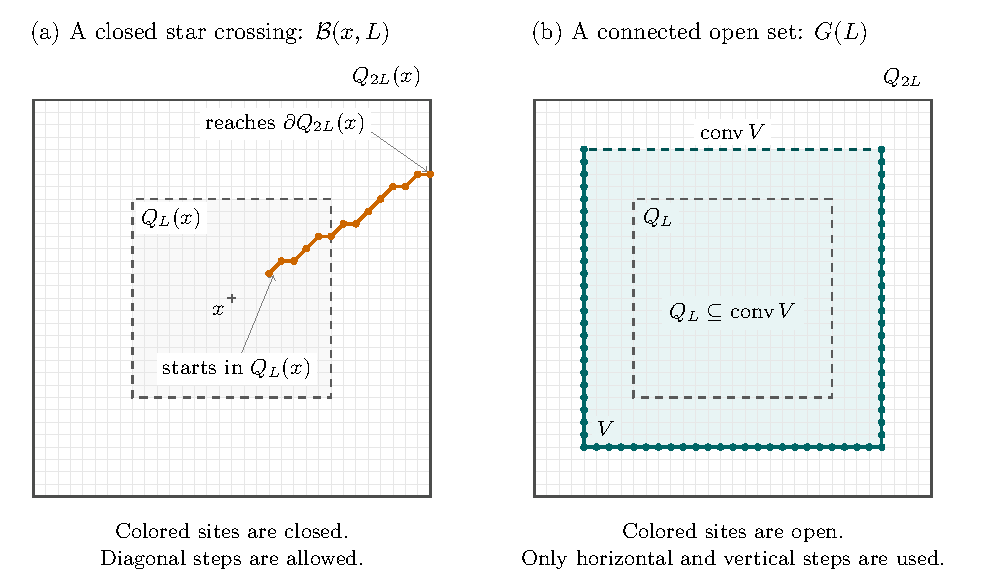
\includegraphics[width=\textwidth]{figures/fig_lattice_events.pdf}
  \caption{The events in \eqref{eq:bad-crossing} and \eqref{eq:initial-open-set}, illustrated with lattice spacing $h=L/8$. Only the coloured sites have specified states. (a)~A closed star path lies in $Q_{2L}(x)$, starts in $Q_L(x)$, and reaches $\partial Q_{2L}(x)$; diagonal steps are permitted. (b)~The open sites form a nearest-neighbour connected set $V\subseteq Q_{2L}$. Its convex hull, shaded in teal, contains $Q_L$. The set $V$ has no cycle, which illustrates that the definition of $G(L)$ requires only connectedness and convex-hull containment. The dashed top edge belongs to the convex hull, not to $V$.}
  \label{fig:lattice-events}
\end{figure}

The two conclusions of the initial estimate must continue to hold when some directions have been deleted. For a measurable set $E\subseteq[0,\pi)$, let $\P_E$ denote the same construction with line intensity measure $\1\{\theta\in E\}\nu_\mu(\d\theta\,\d s)$. The parameters $\mu,\lambda,r$ remain fixed, and the angular density is not renormalised after restriction. The original isotropic law is $\P=\P_{[0,\pi)}$, and $\lvert E\rvert$ denotes the Lebesgue measure of an angular set. By the restriction theorem for Poisson processes~\cite[Theorem~5.2]{LP17}, deleting all lines with normal angles outside~$E$, together with their points, gives precisely the law~$\P_E$. Using the same point configurations on the remaining lines couples the restricted point process to the original one by inclusion.

The first proposition bounds the failure probabilities $\P_E(\cB(0,L))$ and $\P_E(G(L)^\c)$ uniformly over these restrictions. Its two terms correspond to the two stages of the construction: finding lines that form a polygon around the inner square and then obtaining sufficiently dense points along them.

\begin{proposition}[Uniform initial-scale estimate]
\label{prop:initial}
There are universal constants $c,C_0>0$ such that, whenever $\lvert[0,\pi)\setminus E\rvert\le10^{-3}$ and $L\in h\N$ with $L\ge r$,
\begin{equation*}
  \max\bigl\{\P_E(\cB(0,L)),\ \P_E(G(L)^\c)\bigr\}\le C_0\e^{-c\mu L}+C_0(1+L/r)\e^{-c\lambda r}\,.
\end{equation*}
\end{proposition}
All proofs are presented in Section~\ref{sec:initial}. 
Increasing~$L$ makes the environmental term $C_0\e^{-c\mu L}$ small, but also increases the factor $1+L/r$ in the point-process term. Thus, we first choose $L$ of order $\max(r,1/\mu)$, so that the line environment supplies the polygon with high probability, and only then choose $\lambda$ so large that every interval of length of order~$r$ on the selected chords in~$Q_{2L}$ contains a point. This order of choices is responsible for the logarithm in the final intensity bound.

The recursion compares one crossing at scale~$L_{n+1}$ with two crossings at scale~$L_n$. Making those smaller crossings independent removes further directions, so the estimate at the smaller scale must allow a larger total angular loss. We choose the allowances to include every deletion that can occur in repeated comparisons, with their total still below the threshold in Proposition~\ref{prop:initial}.

Fix the universal integer $A\coloneqq2^{20}$. For $n\ge0$, set
\begin{equation}\label{eq:scales-angular-loss}
  a_n\coloneqq A(n+1)^2,\qquad L_{n+1}\coloneqq a_nL_n,\qquad\delta_n\coloneqq64\sum_{k=n}^\infty a_k^{-1}\,.
\end{equation}
Here $L_0\in h\N$ and $L_0\ge r$ will be chosen in the proof. Thus, $L_n=L_0A^n(n!)^2$, $\delta_n=\delta_{n+1}+64/a_n$, and $\delta_0<10^{-3}$. Define
\begin{equation}\label{eq:uniform-crossing-probability}
  \begin{aligned}
    \cE_n\coloneqq\bigl\{E\subseteq[0,\pi)\colon E\text{ is measurable and }\lvert[0,\pi)\setminus E\rvert\le\delta_n\bigr\}\quad\text{and}\quad
    q_n\coloneqq\sup_{E\in\cE_n}\P_E(\cB(0,L_n))\,.
  \end{aligned}
\end{equation}
Each law~$\P_E$ is translation invariant, so $q_n$ also bounds these probabilities at every lattice translate. The identity for~$\delta_n$ allows a law in~$\cE_{n+1}$ to lose at most $64/a_n$ radians and still belong to~$\cE_n$. The next proposition uses precisely this allowance to bound two smaller crossings by independent events.

\begin{proposition}[Recursion by deletion of directions]
\label{prop:recursion}
For every $n\ge0$,
\begin{equation*}
  q_{n+1}\le2401\,a_n^4q_n^2\,.
\end{equation*}
\end{proposition}

The factor $2401\,a_n^4$ counts the pairs of positions of the two smaller crossings; the square~$q_n^2$ reflects their independence after the deletion.

The final comparison concerns a possible exterior boundary of the open set supplied by $G(4L_0)$. If its full open cluster were finite, that boundary would be a finite star-connected set of closed sites whose convex hull contains~$Q_{4L_0}$. Define the boundary event and the desired lattice percolation event by
\begin{equation}\label{eq:boundary-percolation-events}
  \begin{aligned}
    \cD(4L_0)&\coloneqq\Bigg\{
      \begin{gathered}
        \text{there is a finite star-connected closed set}\ T\subseteq h\Z^2\\
        \text{such that }Q_{4L_0}\subseteq\conv T
      \end{gathered}
    \Bigg\},\\
    \cP&\coloneqq\{\text{there is an infinite nearest-neighbour open cluster}\}\,.
  \end{aligned}
\end{equation}
The event~$\cD(4L_0)$ allows every finite closed set with the specified properties, whether or not it is the exterior boundary of an open cluster. Bounding this larger event will therefore control all the boundaries relevant to $G(4L_0)$. The proof of Theorem~\ref{thm:main} will bound $\P(\cD(4L_0))$ by a sum of crossing probabilities. We first state the deterministic relation between~$G(4L_0)$, $\cD(4L_0)$, and~$\cP$.

The geometric relation between the initial open set and percolation is isolated in the following deterministic lemma. Its role is to show that a finite open cluster containing the set in~$G(4L_0)$ forces the closed boundary event~$\cD(4L_0)$.

\begin{lemma}[Deterministic boundary reduction]
\label{lem:boundary-reduction}
For every $L_0\in h\N$ with $L_0\ge r$,
\begin{equation*}
  G(4L_0)\setminus\cD(4L_0)\subseteq\cP\,.
\end{equation*}
\end{lemma}

It remains to explain why positive probability of percolation implies probability one. We use two standard ergodicity results for this purpose. A stationary Poisson hyperplane process with positive intensity is mixing when its directional distribution assigns zero mass to every great subsphere, by Hug and Schneider~\cite[Theorem~7.1.4]{HS24}. In the plane this condition means that each individual unoriented direction has probability zero, so it holds for the uniform angular law in \eqref{eq:line-intensity}.

Consequently, $\cL$ is ergodic under translations. The map from $\cL$ to the line-length measure $\Lambda$ is measurable and commutes with translations, so $\Lambda$ and $\lambda\Lambda$ are ergodic as well. A stationary Cox process directed by an ergodic random measure is ergodic; see Jahnel and K\"onig~\cite[Exercise~6.4.14]{JK20}. Thus, $X_\lambda$ is ergodic, and every translation-invariant event determined by $X_\lambda$ has probability zero or one~\cite[Exercise~6.4.10]{JK20}. In particular,
\begin{equation}\label{eq:percolation-zero-one}
  \P(\Xi_\lambda\text{ percolates})\in\{0,1\}\,.
\end{equation}

\subsection{Proof of \texorpdfstring{Theorem~\ref{thm:main}}{the main theorem}}

We first apply Lemma~\ref{lem:boundary-reduction} to compare the percolation probability with the probabilities of $G(4L_0)$ and~$\cD(4L_0)$. We then cover~$\cD(4L_0)$ by closed crossings and count their possible centres at each scale. This reduces the proof to making $G(4L_0)$ likely and the weighted sum of crossing probabilities small with the same choices of parameters. The recursion turns an initial bound $q_0\le\varepsilon$ into the doubly exponential decay $q_n\le\exp(-t2^n)$ provided that $\varepsilon$ is small enough to absorb the growing prefactors $2401\,a_n^4$. Proposition~\ref{prop:initial} supplies such a small~$\varepsilon$ once the initial scale~$L_0$ and the intensity~$\lambda$ are large, and the logarithm in Theorem~\ref{thm:main} is the price of choosing $L_0$ of order $1/\mu$ when the lines are sparse.

\begin{proof}[Proof of Theorem~\ref{thm:main}]
Fix $\mu,r>0$. For any $\lambda>0$ and any admissible initial scale~$L_0$, Lemma~\ref{lem:boundary-reduction} gives $G(4L_0)\setminus\cD(4L_0)\subseteq\cP$, and hence $\P(\cP)\ge\P(G(4L_0))-\P(\cD(4L_0))$. We bound~$\P(\cD(4L_0))$ by covering the event with closed crossings. Suppose $\cD(4L_0)$ occurs and let~$T$ be a finite star-connected set of closed sites with $Q_{4L_0}\subseteq\conv T$. Write $d\coloneqq\max\{\lVert z-w\rVert_\infty\colon z,w\in T\}$ for its maximum-norm diameter. Since~$\conv T$ contains $[-4L_0,4L_0]$, we have $d\ge8L_0$ and $T\subseteq Q_d$. 

The scales increase strictly to infinity. Choose the unique $n\ge0$ with $8L_n\le d<8L_{n+1}$, and choose $z,w\in T$ attaining the diameter. Round~$z$ to a centre $x\in L_n\Z^2$ with $\lVert x-z\rVert_\infty\le L_n/2$. Then $\lVert x\rVert_\infty\le d+L_n/2<9L_{n+1}$, while $z\in Q_{L_n}(x)$ and $\lVert w-x\rVert_\infty\ge d-L_n/2>2L_n$.
Star-connectedness of~$T$ supplies a finite closed star path from~$z$ to~$w$. Keep the path up to its first visit to~$\partial Q_{2L_n}(x)$. Such a visit occurs because the starting site is inside the inner square, the terminal site is outside the outer square, and a star step cannot skip a boundary at an integer multiple of~$h$. The truncated path stays in~$Q_{2L_n}(x)$ and gives~$\cB(x,L_n)$.

We have therefore covered~$\cD(4L_0)$ by crossings centred at $x\in L_n\Z^2\cap Q_{9L_{n+1}}$ for some $n\ge0$. This is a countable deterministic family, even though the choice of~$T$ and its scale depends on the configuration. At scale~$n$, the number of possible centres is $(18a_n+1)^2\le361a_n^2$. The full angular set $[0,\pi)$ belongs to every~$\cE_n$, so translation invariance gives $\P(\cB(x,L_n))\le q_n$. Consequently,
\begin{equation}\label{eq:boundary-crossing-bound}
  \P(\cD(4L_0))\le\sum_{n=0}^\infty\ \sum_{x\in L_n\Z^2\cap Q_{9L_{n+1}}}\P(\cB(x,L_n))\le361\sum_{n=0}^\infty a_n^2q_n\,.
\end{equation}
The crossing bound holds whether or not the series is finite. We now determine how small the crossing probabilities must be for $\P(\cP)$ to be positive. This requirement fixes universal constants before the line density and radius enter the construction. The scale ratios $a_n=A(n+1)^2$ are fixed universal numbers. The recursion has the form $q_{n+1}\le b_nq_n^2$ with $b_n\coloneqq2401a_n^4$. Repeated squaring gives the logarithm of each factor a weight $2^{-n-1}$, so we put $\sigma\coloneqq\sum_{n=0}^\infty2^{-n-1}\log b_n$. The identity $\log b_n=\log(2401A^4)+8\log(n+1)$ shows that $\sigma<\infty$.

For $t\ge1$, the series $\sum_{n\ge0}a_n^2\exp(-t2^n)$ is dominated by the convergent series $\sum_{n\ge0}a_n^2\exp(-2^n)$ and tends to zero as $t\to\infty$. Choose a universal $t\ge1$ with $361\sum_{n\ge0}a_n^2\exp(-t2^n)<1/4$, and set $\varepsilon\coloneqq\min(1/4,\exp(-\sigma-t))$. These choices depend only on the constants in the recursion and boundary estimate.

We next choose the initial scale so that the line environment supplies the polygon with sufficiently high probability. Once this scale has been fixed, the point intensity will make gaps along the four selected lines unlikely. Let $c,C_0$ be the constants supplied by Proposition~\ref{prop:initial}. Choose a universal $M\ge1$ such that $C_0\exp(-cM)\le\varepsilon/2$, and put $K\coloneqq11/2+4M$. The initial scale is at least both the disk radius and a constant multiple of $1/\mu$. We choose the point intensity to absorb the resulting factor $1+4L_0/r$ in the initial estimate:
\begin{align}\label{eq:parameter-choice}
  L_0&\coloneqq h\bigl\lceil\max(r,M/\mu)/h\bigr\rceil,&C_1&\coloneqq\frac1c\max\{1,\log(2C_0K/\varepsilon)\},\\
  \lambda&\ge\frac{C_1}{r}\bigl[1+\logp(1/(\mu r))\bigr],&1+4L_0/r&\le K\max\{1,1/(\mu r)\}\,.\notag
\end{align}
Indeed, the definition of~$L_0$ gives $L_0\in h\N$, $L_0\ge r$, $\mu L_0\ge M$, and $L_0/r\le9/8+M/(\mu r)$, which proves the last inequality. To check the point-process term, put $u\coloneqq\logp(1/(\mu r))$. The definition of~$C_1$ implies $cC_1(1+u)\ge\log(2C_0K/\varepsilon)+u$, and consequently $C_0(1+4L_0/r)\exp(-c\lambda r)\le\varepsilon/2$.

These choices must supply two initial bounds: a uniform estimate for the closed crossing at~$L_0$ and a high probability for the open set at~$4L_0$. We check the hypotheses of Proposition~\ref{prop:initial} at each scale. Every $E\in\cE_0$ satisfies $\lvert[0,\pi)\setminus E\rvert\le\delta_0<10^{-3}$. Applying Proposition~\ref{prop:initial} at~$L_0$, the environmental term is at most $C_0\exp(-cM)\le\varepsilon/2$, and the point-process term is bounded by its value with $4L_0$ in place of~$L_0$. Thus, $\P_E(\cB(0,L_0))\le\varepsilon$ uniformly over~$\cE_0$, giving $q_0\le\varepsilon$. Apply the same proposition with $E=[0,\pi)$ and scale~$4L_0$. The scale belongs to~$h\N$ and is at least~$r$, the environmental term has decreased, and the point-process term is the one already estimated. We obtain $\P(G(4L_0))\ge1-\varepsilon$.

We can now propagate the crossing bound to all scales and substitute it into the exterior boundary estimate. Proposition~\ref{prop:recursion} applies successively at every scale with $\mu,r$ fixed and with $\lambda,L_0$ as in \eqref{eq:parameter-choice}. If $q_0=0$, it gives $q_n=0$ for all~$n$. Otherwise, substituting each bound into the next and using $q_0\le\e^{-\sigma-t}$ yields
\begin{align}\label{eq:iterated-crossing-bound}
  q_n&\le q_0^{2^n}\prod_{j=0}^{n-1}b_j^{2^{n-1-j}}\le\exp\Bigl(-2^n\Bigl[\sigma+t-\sum_{j=0}^{n-1}2^{-j-1}\log b_j\Bigr]\Bigr)\le\e^{-t2^n},
  \end{align}
where for $n=0$ the product is empty and equals one. Hence,
\begin{align*}
  \P(\cP)\ge\P(G(4L_0))-361\sum_{n=0}^\infty a_n^2q_n\ge1-\varepsilon-361\sum_{n=0}^\infty a_n^2\e^{-t2^n}>\frac12
\end{align*}
and the lattice comparison following \eqref{eq:site-states} now gives positive probability of Boolean percolation. Since every~$\lambda$ satisfying \eqref{eq:parameter-choice} has been covered, the asserted bound on~$\lambda_c$ follows with $C=C_1$. The zero--one conclusion in \eqref{eq:percolation-zero-one} upgrades this positive probability to one.
\end{proof}

% =================================================================
\section{Proof of \texorpdfstring{Proposition~\ref{prop:recursion}}{the recursion}: deleting directions}
\label{sec:recursion}

We begin with the coupling and independence argument that gives the recursion. Two geometric facts suffice: a large closed crossing produces two separated smaller crossings from a controlled finite family, and the directions of lines meeting both smaller windows occupy an angular set of measure at most $64/a_n$. We state these facts precisely and derive the probability bound before verifying either construction. The extraction of the smaller crossings follows the geometric argument in Gou\'er\'e~\cite[Lemma~3.3]{Gou08}, applied here to closed lattice paths; see Figure~\ref{fig:recursion}. We then construct the angular set, show that it removes every line shared by the windows, and verify its measure bound.

\begin{figure}[ht]
  \centering
  % Generated by make_figures.py (fig_recursion) -- do not edit by hand.
% L = 1, a = 6 (in the proof a >= 2^20); schematic path.
\begin{tikzpicture}[x=0.4cm,y=0.4cm]
  \begin{scope}
    \clip (-14.5,-13) rectangle (15.5,15.5);
    \foreach \i in {-18,...,18} \foreach \j in {-18,...,18} \fill[gray!45] (\i,\j) circle (0.06);
  \end{scope}
  \node[anchor=south west, font=\small] at (-6,-6) {$Q_R$};
  \node[anchor=south west, font=\small] at (-12,-12) {$Q_{2R}$};
  \fill[retainedfill!45] (3.0,2.0) rectangle (9.0,8.0);
  \fill[retainedfill!45] (9.0,7.0) rectangle (15.0,13.0);
  \draw[thick] (-6,-6) rectangle (6,6);
  \draw[thick] (-12,-12) rectangle (12,12);
  \draw[gray, dashed] (3.0,2.0) rectangle (9.0,8.0);
  \draw[retained] (4.0,3.0) rectangle (8.0,7.0);
  \draw[retained] (5.0,4.0) rectangle (7.0,6.0);
  \fill[retained] (6.0,5.0) circle (0.18) node[above right=-2pt, font=\small] {$x$};
  \draw[gray, dashed] (9.0,7.0) rectangle (15.0,13.0);
  \draw[retained] (10.0,8.0) rectangle (14.0,12.0);
  \draw[retained] (11.0,9.0) rectangle (13.0,11.0);
  \fill[retained] (12.0,10.0) circle (0.18) node[below right=-2pt, font=\small] {$y$};
  \draw[deleted, densely dashed, thick] (-3.000,-1.500) -- (-1.000,0.500) -- (1.500,0.000) -- (2.500,2.500) -- (4.500,3.000) -- (5.000,4.500) -- (6.000,4.600) -- (7.200,5.600) -- (7.600,7.400) -- (9.400,8.000) -- (10.200,9.600) -- (11.200,10.000) -- (12.000,10.300);
  \draw[deleted, line width=1.6pt] (6.000,4.600) -- (7.200,5.600) -- (7.511,7.000);
  \draw[deleted, line width=1.6pt] (12.000,10.300) -- (11.200,10.000) -- (10.200,9.600) -- (10.000,9.200);
  \fill[black] (6.000,4.600) circle (0.2) node[below left=-2pt, font=\small] {$u$};
  \fill[black] (12.000,10.300) circle (0.2) node[above left=-1pt, font=\small] {$v$};
  \node[font=\scriptsize, anchor=north] at (6.000,2.000) {$Q_{3L}(x)$};
  \node[font=\scriptsize, anchor=south] at (12.000,13.000) {$Q_{3L}(y)$};
\end{tikzpicture}

  \caption{Extraction of two crossings in the proof of Proposition~\ref{prop:recursion}, schematic with $L=1$ and $a=6$; the proof uses $a\ge2^{20}$. Grey dots form the coarse lattice~$L\Z^2$. The dashed closed path joins~$Q_R$ to~$\partial Q_{2R}$. A vertex $u\in\partial Q_R$ and a later vertex $v\in\partial Q_{2R}$ are rounded to the centres $x,y\in L\Z^2$. The thick parts give the crossings in $\cB(x,L)$ and~$\cB(y,L)$: they join $Q_L(x)$ to~$\partial Q_{2L}(x)$ inside~$Q_{2L}(x)$, and similarly for~$y$. The shaded windows $Q_{3L}(x)$ and $Q_{3L}(y)$ determine the two events. Deleting all directions that permit a line to meet both windows makes the two configurations independent, as in Figure~\ref{fig:deletion}.}
  \label{fig:recursion}
\end{figure}

\begin{proof}[Proof of Proposition~\ref{prop:recursion}]
Fix an integer $n\ge0$ and write $L\coloneqq L_n$, $a\coloneqq a_n$, and $R\coloneqq L_{n+1}=aL$. Let $E\in\cE_{n+1}$. Let $\cK$ be the set of all pairs $(x,y)$ with $x,y\in L\Z^2\cap Q_{3R}$ and $\lVert x-y\rVert_\infty\ge(a-1)L$. This finite set does not depend on the configuration. Put $W_z\coloneqq Q_{3L}(z)$ for $z\in L\Z^2$. The event~$\cB(z,L)$ is determined by the points in~$W_z$, as shown after \eqref{eq:bad-crossing}.

\emph{Step 1: Reduction by coupling and independence.} We first state the two geometric facts needed for the probability estimate. The first is the covering and counting bound
\begin{equation}\label{eq:recursion-geometric-cover}
  \cB(0,R)\subseteq\bigcup_{(x,y)\in\cK}\bigl(\cB(x,L)\cap\cB(y,L)\bigr),\qquad\#\cK\le2401a^4\,.
\end{equation}
The second is that, for every $(x,y)\in\cK$, there is a deterministic measurable set $I=I(x,y)\subseteq[0,\pi)$ with $\lvert I\rvert\le64/a$ that contains the normal angle of every line meeting both~$W_x$ and~$W_y$. We will prove the covering bound in Step~2 and construct this angular set in Step~3. We now show in full how these two facts imply the proposition.

Fix a pair $(x,y)\in\cK$ and an angular set~$I$ with the stated properties, and put $E'\coloneqq E\setminus I$. Since $E\in\cE_{n+1}$, the loss of directions satisfies $\lvert[0,\pi)\setminus E'\rvert\le\delta_{n+1}+64/a=\delta_n$, so $E'\in\cE_n$. Start with the marked lines under~$\P_E$, delete those whose angles belong to~$I$, and keep all points on the other lines. The restriction and marking properties described in Sections~\ref{sec:setting} and~\ref{sec:lattice-events} give exactly the law~$\P_{E'}$ for this configuration. In particular, the angular density remains~$\mu/\pi$ on~$E'$. Since deletion removes points, each closed crossing present before deletion remains a closed crossing afterwards. Thus, this coupling bounds the probability of the original pair of crossings by its probability under~$\P_{E'}$.

To obtain independence under~$\P_{E'}$, let $\cA_x$ be the set of line parameters $(\theta,s)$ with $\theta\in E'$ and $\ell(\theta,s)\cap W_x\neq\varnothing$, and define~$\cA_y$ in the same way. These measurable sets are disjoint: a line meeting both windows would have its normal angle in~$I$, whereas $E'\cap I=\varnothing$. The restrictions of the marked Poisson process to~$\cA_x$ and~$\cA_y$ are therefore independent. Every point that can affect~$\cB(x,L)$ lies on a line from~$\cA_x$, and the points on that line are included in the corresponding restriction; the same assertion holds for~$y$. Hence, the two crossing events are independent under~$\P_{E'}$. Both marginal laws come from the stationary model with angular set~$E'$, so translation invariance and $E'\in\cE_n$ give
\begin{align}\label{eq:recursion-probability-reduction}
  \P_E\bigl(\cB(x,L)\cap\cB(y,L)\bigr)&\le\P_{E'}\bigl(\cB(x,L)\cap\cB(y,L)\bigr)=\P_{E'}(\cB(x,L))\,\P_{E'}(\cB(y,L))\le q_n^2,\\
  \P_E(\cB(0,R))&\le\sum_{(x,y)\in\cK}\P_E\bigl(\cB(x,L)\cap\cB(y,L)\bigr)\le2401a^4q_n^2\,.\notag
\end{align}
The second line uses \eqref{eq:recursion-geometric-cover} and a union bound. The first line is proved separately for each deterministic pair, so each pair may use its own angular set~$I$ and hence its own law~$\P_{E'}$. The same supremum~$q_n$ bounds every such law. In particular, the angular losses are not added over the pairs in~$\cK$, and no conditioning on a randomly selected pair is involved. Taking the supremum over $E\in\cE_{n+1}$ gives $q_{n+1}\le2401a_n^4q_n^2$. It remains to verify the two geometric facts used in this deduction.

\emph{Step 2: Two separated crossings.} On~$\cB(0,R)$, choose a finite closed star path from a site of~$Q_R$ to~$\partial Q_{2R}$, contained in~$Q_{2R}$. Because $R$ and the site coordinates are integer multiples of~$h$, a star step changes each coordinate by at most~$h$ and cannot jump across a lattice boundary without hitting it. The path therefore has a vertex $u\in\partial Q_R$ followed by a vertex $v\in\partial Q_{2R}$. Restrict attention to the segment of the path between these two vertices. Their maximum-norm distance is at least~$R$: in a coordinate where $v$ has absolute value~$2R$, the corresponding coordinate of~$u$ has absolute value at most~$R$.

Round each coordinate of $u$ and~$v$ to a nearest multiple of~$L$, using a fixed convention for ties, to obtain $x,y\in L\Z^2$ with $\lVert x-u\rVert_\infty,\lVert y-v\rVert_\infty\le L/2$. Since $L\in h\N$, these centres are also sites of~$h\Z^2$. They lie in~$Q_{3R}$, and $\lVert x-y\rVert_\infty\ge R-L=(a-1)L$, so $(x,y)\in\cK$. The point~$u$ lies in~$Q_L(x)$, whereas $\lVert v-x\rVert_\infty\ge R-L/2>2L$. Truncating the path at its first visit to~$\partial Q_{2L}(x)$ gives a closed crossing in~$\cB(x,L)$. Applying the same argument to the reverse path starting at~$v$ gives a crossing in~$\cB(y,L)$. In both cases the exact boundary is reached because its coordinates are multiples of~$h$.

This proves the inclusion in \eqref{eq:recursion-geometric-cover}. Since $a$ is an integer, there are $(6a+1)^2\le49a^2$ possible centres in $L\Z^2\cap Q_{3R}$, and hence $\#\cK\le(49a^2)^2=2401a^4$. Both parts of the covering and counting bound are now established.

\emph{Step 3: The deleted directions.} Fix $(x,y)\in\cK$ and put $d\coloneqq\lVert x-y\rVert_2$. We choose $I\coloneqq\{\theta\in[0,\pi)\colon\lvert(x-y)\cdot n_\theta\rvert\le6\sqrt2L\}$. This set is measurable and depends only on the fixed centres and scale. To check that it contains every direction shared by the two windows, suppose $\ell(\theta,s)$ meets~$W_x$ at~$p$ and~$W_y$ at~$q$. Since $p\cdot n_\theta=q\cdot n_\theta=s$, we have $\lvert(x-y)\cdot n_\theta\rvert\le\lVert x-p\rVert_2+\lVert q-y\rVert_2\le6\sqrt2L$. Thus, the normal angle of any line meeting both windows belongs to~$I$. The definition includes the endpoint angles, so lines at equality are removed as well.

It remains to check that the angular set is small enough. Write $x-y=d(\cos\varphi,\sin\varphi)$ for some angle~$\varphi$. The inequality defining~$I$ is $\lvert\cos(\theta-\varphi)\rvert\le6\sqrt2L/d$. Since $d\ge(a-1)L$ and $a\ge A>100$, its right-hand side is less than~$1/2$. Over an interval of length~$\pi$, this condition selects an angular interval, possibly split at~$0$, of total length $2\arcsin(6\sqrt2L/d)$. Using $\arcsin t\le2t$ for $0\le t\le1/2$, we obtain
\begin{equation}\label{eq:recursion-angular-bound}
  \lvert I\rvert=2\arcsin(6\sqrt2L/d)\le\frac{24\sqrt2L}{d}\le\frac{24\sqrt2}{a-1}\le\frac{64}{a}\,.
\end{equation}
The last inequality holds for $a\ge100$. This verifies the second geometric fact and completes the reduction in Step~1, proving the proposition.
\end{proof}

% =================================================================
\section{Proof of \texorpdfstring{Proposition~\ref{prop:initial}}{the initial estimate}: the initial estimate}
\label{sec:initial}

We prove the initial estimate by constructing one event $\cH$ that gives both conclusions: a closed crossing is impossible, and a sufficiently large connected open set exists. The event requires four lines forming a polygon around the inner square and sufficiently dense points on those lines. After defining the construction, we state its two geometric consequences in an auxiliary lemma and prove the proposition by estimating the line counts and point gaps. The proof of the geometric lemma is deferred to Section~\ref{sec:geometry}, where it appears with the exterior-boundary argument.

Fix an angular set $E$ and a scale $L$ satisfying the hypotheses of Proposition~\ref{prop:initial}, and put $\eta\coloneqq1/100$. Let $\cF_T$ consist of lines $y=a+bx$ with $\lvert b\rvert\le\eta$ and $a\in[1.4L,1.5L]$, and let $\cF_B$ use $a\in[-1.5L,-1.4L]$ with the same slope range. Define $\cF_R$ and $\cF_L$ by the equations $x=a+by$ with these positive and negative intercept ranges, respectively. In all four families, include only lines whose normal angles belong to~$E$. The letters $T,B,R,L$ specify the top, bottom, right, and left sides of the polygon. Three lines in general position would already enclose a bounded region. We use four families aligned with the coordinate axes because the resulting polygon fits between $Q_{1.3L}$ and $Q_{1.6L}$, and the required inclusions can be checked coordinatewise.

Let $\cA$ be the event that all four families contain a line. On~$\cA$, choose the line with the smallest normal angle from each family, breaking a tie by its displacement, and denote its coefficients by $(a_i,b_i)$ for $i\in\{T,B,R,L\}$. This choice uses only the line environment. Define $P$ as the intersection of the four inward half-planes, so that a point $w=(w_1,w_2)$ belongs to $P$ exactly when
\begin{equation}\label{eq:polygon-definition}
  \begin{aligned}
    w_2\le a_T+b_Tw_1,\  w_2\ge a_B+b_Bw_1,\  w_1\le a_R+b_Rw_2,\ w_1\ge a_L+b_Lw_2\,.
  \end{aligned}
\end{equation}
Write $\Gamma\coloneqq\partial P$. Each selected line passes through the interior of $Q_{2L}$ and therefore has a chord of positive length~$\ell_i$ in this square. Divide this chord into $N_i\coloneqq\lceil16\ell_i/r\rceil$ equal arclength intervals, using half-open intervals with the final endpoint included in the last interval. Orient the chord from its lexicographically smaller endpoint to fix the partition convention. The event requiring points along all four chords is
\begin{equation}\label{eq:successful-polygon}
  \cH\coloneqq\cA\cap\Bigg\{
    \begin{gathered}
      \text{every interval in the four chosen partitions contains}\\
      \text{a point of the Poisson process on its selected line}
    \end{gathered}
  \Bigg\}\,.
\end{equation}
The partitions in \eqref{eq:successful-polygon} are defined on~$\cA$, and $\cH$ is declared false on~$\cA^\c$. For $z\in h\Z^2$, put $D_z\coloneqq z+[-h/2,h/2]^2$, and on~$\cA$ let $V\coloneqq\{z\in h\Z^2\colon D_z\cap\Gamma\neq\varnothing\}$. Thus, $V$ consists of the centres of the closed lattice tiles meeting the polygon boundary. Figure~\ref{fig:polygon} shows the construction.

\begin{figure}[ht]
  \centering
  % Generated by make_figures.py (fig_polygon) -- do not edit by hand.
% L = r = 1, h = 1/8; slopes enlarged to at most 1/20 (inclusions re-checked).
\begin{tikzpicture}[x=2.1cm,y=2.1cm]
  \fill[retainedfill!55] (-1.562,-1.438) rectangle ++(0.125,0.125);
  \fill[retainedfill!55] (-1.562,-1.312) rectangle ++(0.125,0.125);
  \fill[retainedfill!55] (-1.562,-1.188) rectangle ++(0.125,0.125);
  \fill[retainedfill!55] (-1.562,-1.062) rectangle ++(0.125,0.125);
  \fill[retainedfill!55] (-1.562,-0.938) rectangle ++(0.125,0.125);
  \fill[retainedfill!55] (-1.562,-0.812) rectangle ++(0.125,0.125);
  \fill[retainedfill!55] (-1.562,-0.688) rectangle ++(0.125,0.125);
  \fill[retainedfill!55] (-1.562,-0.562) rectangle ++(0.125,0.125);
  \fill[retainedfill!55] (-1.562,-0.438) rectangle ++(0.125,0.125);
  \fill[retainedfill!55] (-1.438,-1.438) rectangle ++(0.125,0.125);
  \fill[retainedfill!55] (-1.438,-0.438) rectangle ++(0.125,0.125);
  \fill[retainedfill!55] (-1.438,-0.312) rectangle ++(0.125,0.125);
  \fill[retainedfill!55] (-1.438,-0.188) rectangle ++(0.125,0.125);
  \fill[retainedfill!55] (-1.438,-0.062) rectangle ++(0.125,0.125);
  \fill[retainedfill!55] (-1.438,0.062) rectangle ++(0.125,0.125);
  \fill[retainedfill!55] (-1.438,0.188) rectangle ++(0.125,0.125);
  \fill[retainedfill!55] (-1.438,0.312) rectangle ++(0.125,0.125);
  \fill[retainedfill!55] (-1.438,0.438) rectangle ++(0.125,0.125);
  \fill[retainedfill!55] (-1.438,0.562) rectangle ++(0.125,0.125);
  \fill[retainedfill!55] (-1.438,0.688) rectangle ++(0.125,0.125);
  \fill[retainedfill!55] (-1.438,0.812) rectangle ++(0.125,0.125);
  \fill[retainedfill!55] (-1.438,0.938) rectangle ++(0.125,0.125);
  \fill[retainedfill!55] (-1.438,1.062) rectangle ++(0.125,0.125);
  \fill[retainedfill!55] (-1.438,1.188) rectangle ++(0.125,0.125);
  \fill[retainedfill!55] (-1.438,1.312) rectangle ++(0.125,0.125);
  \fill[retainedfill!55] (-1.312,-1.438) rectangle ++(0.125,0.125);
  \fill[retainedfill!55] (-1.312,1.312) rectangle ++(0.125,0.125);
  \fill[retainedfill!55] (-1.188,-1.438) rectangle ++(0.125,0.125);
  \fill[retainedfill!55] (-1.188,1.312) rectangle ++(0.125,0.125);
  \fill[retainedfill!55] (-1.062,-1.438) rectangle ++(0.125,0.125);
  \fill[retainedfill!55] (-1.062,1.312) rectangle ++(0.125,0.125);
  \fill[retainedfill!55] (-0.938,-1.438) rectangle ++(0.125,0.125);
  \fill[retainedfill!55] (-0.938,1.312) rectangle ++(0.125,0.125);
  \fill[retainedfill!55] (-0.812,-1.438) rectangle ++(0.125,0.125);
  \fill[retainedfill!55] (-0.812,1.312) rectangle ++(0.125,0.125);
  \fill[retainedfill!55] (-0.688,-1.438) rectangle ++(0.125,0.125);
  \fill[retainedfill!55] (-0.688,1.312) rectangle ++(0.125,0.125);
  \fill[retainedfill!55] (-0.562,-1.438) rectangle ++(0.125,0.125);
  \fill[retainedfill!55] (-0.562,1.312) rectangle ++(0.125,0.125);
  \fill[retainedfill!55] (-0.438,-1.438) rectangle ++(0.125,0.125);
  \fill[retainedfill!55] (-0.438,1.312) rectangle ++(0.125,0.125);
  \fill[retainedfill!55] (-0.312,-1.438) rectangle ++(0.125,0.125);
  \fill[retainedfill!55] (-0.312,1.312) rectangle ++(0.125,0.125);
  \fill[retainedfill!55] (-0.312,1.438) rectangle ++(0.125,0.125);
  \fill[retainedfill!55] (-0.188,-1.438) rectangle ++(0.125,0.125);
  \fill[retainedfill!55] (-0.188,1.438) rectangle ++(0.125,0.125);
  \fill[retainedfill!55] (-0.062,-1.438) rectangle ++(0.125,0.125);
  \fill[retainedfill!55] (-0.062,1.438) rectangle ++(0.125,0.125);
  \fill[retainedfill!55] (0.062,-1.438) rectangle ++(0.125,0.125);
  \fill[retainedfill!55] (0.062,1.438) rectangle ++(0.125,0.125);
  \fill[retainedfill!55] (0.188,-1.562) rectangle ++(0.125,0.125);
  \fill[retainedfill!55] (0.188,-1.438) rectangle ++(0.125,0.125);
  \fill[retainedfill!55] (0.188,1.438) rectangle ++(0.125,0.125);
  \fill[retainedfill!55] (0.312,-1.562) rectangle ++(0.125,0.125);
  \fill[retainedfill!55] (0.312,1.438) rectangle ++(0.125,0.125);
  \fill[retainedfill!55] (0.438,-1.562) rectangle ++(0.125,0.125);
  \fill[retainedfill!55] (0.438,1.438) rectangle ++(0.125,0.125);
  \fill[retainedfill!55] (0.562,-1.562) rectangle ++(0.125,0.125);
  \fill[retainedfill!55] (0.562,1.438) rectangle ++(0.125,0.125);
  \fill[retainedfill!55] (0.688,-1.562) rectangle ++(0.125,0.125);
  \fill[retainedfill!55] (0.688,1.438) rectangle ++(0.125,0.125);
  \fill[retainedfill!55] (0.812,-1.562) rectangle ++(0.125,0.125);
  \fill[retainedfill!55] (0.812,1.438) rectangle ++(0.125,0.125);
  \fill[retainedfill!55] (0.938,-1.562) rectangle ++(0.125,0.125);
  \fill[retainedfill!55] (0.938,1.438) rectangle ++(0.125,0.125);
  \fill[retainedfill!55] (1.062,-1.562) rectangle ++(0.125,0.125);
  \fill[retainedfill!55] (1.062,1.438) rectangle ++(0.125,0.125);
  \fill[retainedfill!55] (1.188,-1.562) rectangle ++(0.125,0.125);
  \fill[retainedfill!55] (1.188,1.438) rectangle ++(0.125,0.125);
  \fill[retainedfill!55] (1.312,-1.562) rectangle ++(0.125,0.125);
  \fill[retainedfill!55] (1.312,0.812) rectangle ++(0.125,0.125);
  \fill[retainedfill!55] (1.312,0.938) rectangle ++(0.125,0.125);
  \fill[retainedfill!55] (1.312,1.062) rectangle ++(0.125,0.125);
  \fill[retainedfill!55] (1.312,1.188) rectangle ++(0.125,0.125);
  \fill[retainedfill!55] (1.312,1.312) rectangle ++(0.125,0.125);
  \fill[retainedfill!55] (1.312,1.438) rectangle ++(0.125,0.125);
  \fill[retainedfill!55] (1.438,-1.562) rectangle ++(0.125,0.125);
  \fill[retainedfill!55] (1.438,-1.438) rectangle ++(0.125,0.125);
  \fill[retainedfill!55] (1.438,-1.312) rectangle ++(0.125,0.125);
  \fill[retainedfill!55] (1.438,-1.188) rectangle ++(0.125,0.125);
  \fill[retainedfill!55] (1.438,-1.062) rectangle ++(0.125,0.125);
  \fill[retainedfill!55] (1.438,-0.938) rectangle ++(0.125,0.125);
  \fill[retainedfill!55] (1.438,-0.812) rectangle ++(0.125,0.125);
  \fill[retainedfill!55] (1.438,-0.688) rectangle ++(0.125,0.125);
  \fill[retainedfill!55] (1.438,-0.562) rectangle ++(0.125,0.125);
  \fill[retainedfill!55] (1.438,-0.438) rectangle ++(0.125,0.125);
  \fill[retainedfill!55] (1.438,-0.312) rectangle ++(0.125,0.125);
  \fill[retainedfill!55] (1.438,-0.188) rectangle ++(0.125,0.125);
  \fill[retainedfill!55] (1.438,-0.062) rectangle ++(0.125,0.125);
  \fill[retainedfill!55] (1.438,0.062) rectangle ++(0.125,0.125);
  \fill[retainedfill!55] (1.438,0.188) rectangle ++(0.125,0.125);
  \fill[retainedfill!55] (1.438,0.312) rectangle ++(0.125,0.125);
  \fill[retainedfill!55] (1.438,0.438) rectangle ++(0.125,0.125);
  \fill[retainedfill!55] (1.438,0.562) rectangle ++(0.125,0.125);
  \fill[retainedfill!55] (1.438,0.688) rectangle ++(0.125,0.125);
  \fill[retainedfill!55] (1.438,0.812) rectangle ++(0.125,0.125);
  \draw[retained!50, very thin] (-1.562,-1.438) rectangle ++(0.125,0.125);
  \draw[retained!50, very thin] (-1.562,-1.312) rectangle ++(0.125,0.125);
  \draw[retained!50, very thin] (-1.562,-1.188) rectangle ++(0.125,0.125);
  \draw[retained!50, very thin] (-1.562,-1.062) rectangle ++(0.125,0.125);
  \draw[retained!50, very thin] (-1.562,-0.938) rectangle ++(0.125,0.125);
  \draw[retained!50, very thin] (-1.562,-0.812) rectangle ++(0.125,0.125);
  \draw[retained!50, very thin] (-1.562,-0.688) rectangle ++(0.125,0.125);
  \draw[retained!50, very thin] (-1.562,-0.562) rectangle ++(0.125,0.125);
  \draw[retained!50, very thin] (-1.562,-0.438) rectangle ++(0.125,0.125);
  \draw[retained!50, very thin] (-1.438,-1.438) rectangle ++(0.125,0.125);
  \draw[retained!50, very thin] (-1.438,-0.438) rectangle ++(0.125,0.125);
  \draw[retained!50, very thin] (-1.438,-0.312) rectangle ++(0.125,0.125);
  \draw[retained!50, very thin] (-1.438,-0.188) rectangle ++(0.125,0.125);
  \draw[retained!50, very thin] (-1.438,-0.062) rectangle ++(0.125,0.125);
  \draw[retained!50, very thin] (-1.438,0.062) rectangle ++(0.125,0.125);
  \draw[retained!50, very thin] (-1.438,0.188) rectangle ++(0.125,0.125);
  \draw[retained!50, very thin] (-1.438,0.312) rectangle ++(0.125,0.125);
  \draw[retained!50, very thin] (-1.438,0.438) rectangle ++(0.125,0.125);
  \draw[retained!50, very thin] (-1.438,0.562) rectangle ++(0.125,0.125);
  \draw[retained!50, very thin] (-1.438,0.688) rectangle ++(0.125,0.125);
  \draw[retained!50, very thin] (-1.438,0.812) rectangle ++(0.125,0.125);
  \draw[retained!50, very thin] (-1.438,0.938) rectangle ++(0.125,0.125);
  \draw[retained!50, very thin] (-1.438,1.062) rectangle ++(0.125,0.125);
  \draw[retained!50, very thin] (-1.438,1.188) rectangle ++(0.125,0.125);
  \draw[retained!50, very thin] (-1.438,1.312) rectangle ++(0.125,0.125);
  \draw[retained!50, very thin] (-1.312,-1.438) rectangle ++(0.125,0.125);
  \draw[retained!50, very thin] (-1.312,1.312) rectangle ++(0.125,0.125);
  \draw[retained!50, very thin] (-1.188,-1.438) rectangle ++(0.125,0.125);
  \draw[retained!50, very thin] (-1.188,1.312) rectangle ++(0.125,0.125);
  \draw[retained!50, very thin] (-1.062,-1.438) rectangle ++(0.125,0.125);
  \draw[retained!50, very thin] (-1.062,1.312) rectangle ++(0.125,0.125);
  \draw[retained!50, very thin] (-0.938,-1.438) rectangle ++(0.125,0.125);
  \draw[retained!50, very thin] (-0.938,1.312) rectangle ++(0.125,0.125);
  \draw[retained!50, very thin] (-0.812,-1.438) rectangle ++(0.125,0.125);
  \draw[retained!50, very thin] (-0.812,1.312) rectangle ++(0.125,0.125);
  \draw[retained!50, very thin] (-0.688,-1.438) rectangle ++(0.125,0.125);
  \draw[retained!50, very thin] (-0.688,1.312) rectangle ++(0.125,0.125);
  \draw[retained!50, very thin] (-0.562,-1.438) rectangle ++(0.125,0.125);
  \draw[retained!50, very thin] (-0.562,1.312) rectangle ++(0.125,0.125);
  \draw[retained!50, very thin] (-0.438,-1.438) rectangle ++(0.125,0.125);
  \draw[retained!50, very thin] (-0.438,1.312) rectangle ++(0.125,0.125);
  \draw[retained!50, very thin] (-0.312,-1.438) rectangle ++(0.125,0.125);
  \draw[retained!50, very thin] (-0.312,1.312) rectangle ++(0.125,0.125);
  \draw[retained!50, very thin] (-0.312,1.438) rectangle ++(0.125,0.125);
  \draw[retained!50, very thin] (-0.188,-1.438) rectangle ++(0.125,0.125);
  \draw[retained!50, very thin] (-0.188,1.438) rectangle ++(0.125,0.125);
  \draw[retained!50, very thin] (-0.062,-1.438) rectangle ++(0.125,0.125);
  \draw[retained!50, very thin] (-0.062,1.438) rectangle ++(0.125,0.125);
  \draw[retained!50, very thin] (0.062,-1.438) rectangle ++(0.125,0.125);
  \draw[retained!50, very thin] (0.062,1.438) rectangle ++(0.125,0.125);
  \draw[retained!50, very thin] (0.188,-1.562) rectangle ++(0.125,0.125);
  \draw[retained!50, very thin] (0.188,-1.438) rectangle ++(0.125,0.125);
  \draw[retained!50, very thin] (0.188,1.438) rectangle ++(0.125,0.125);
  \draw[retained!50, very thin] (0.312,-1.562) rectangle ++(0.125,0.125);
  \draw[retained!50, very thin] (0.312,1.438) rectangle ++(0.125,0.125);
  \draw[retained!50, very thin] (0.438,-1.562) rectangle ++(0.125,0.125);
  \draw[retained!50, very thin] (0.438,1.438) rectangle ++(0.125,0.125);
  \draw[retained!50, very thin] (0.562,-1.562) rectangle ++(0.125,0.125);
  \draw[retained!50, very thin] (0.562,1.438) rectangle ++(0.125,0.125);
  \draw[retained!50, very thin] (0.688,-1.562) rectangle ++(0.125,0.125);
  \draw[retained!50, very thin] (0.688,1.438) rectangle ++(0.125,0.125);
  \draw[retained!50, very thin] (0.812,-1.562) rectangle ++(0.125,0.125);
  \draw[retained!50, very thin] (0.812,1.438) rectangle ++(0.125,0.125);
  \draw[retained!50, very thin] (0.938,-1.562) rectangle ++(0.125,0.125);
  \draw[retained!50, very thin] (0.938,1.438) rectangle ++(0.125,0.125);
  \draw[retained!50, very thin] (1.062,-1.562) rectangle ++(0.125,0.125);
  \draw[retained!50, very thin] (1.062,1.438) rectangle ++(0.125,0.125);
  \draw[retained!50, very thin] (1.188,-1.562) rectangle ++(0.125,0.125);
  \draw[retained!50, very thin] (1.188,1.438) rectangle ++(0.125,0.125);
  \draw[retained!50, very thin] (1.312,-1.562) rectangle ++(0.125,0.125);
  \draw[retained!50, very thin] (1.312,0.812) rectangle ++(0.125,0.125);
  \draw[retained!50, very thin] (1.312,0.938) rectangle ++(0.125,0.125);
  \draw[retained!50, very thin] (1.312,1.062) rectangle ++(0.125,0.125);
  \draw[retained!50, very thin] (1.312,1.188) rectangle ++(0.125,0.125);
  \draw[retained!50, very thin] (1.312,1.312) rectangle ++(0.125,0.125);
  \draw[retained!50, very thin] (1.312,1.438) rectangle ++(0.125,0.125);
  \draw[retained!50, very thin] (1.438,-1.562) rectangle ++(0.125,0.125);
  \draw[retained!50, very thin] (1.438,-1.438) rectangle ++(0.125,0.125);
  \draw[retained!50, very thin] (1.438,-1.312) rectangle ++(0.125,0.125);
  \draw[retained!50, very thin] (1.438,-1.188) rectangle ++(0.125,0.125);
  \draw[retained!50, very thin] (1.438,-1.062) rectangle ++(0.125,0.125);
  \draw[retained!50, very thin] (1.438,-0.938) rectangle ++(0.125,0.125);
  \draw[retained!50, very thin] (1.438,-0.812) rectangle ++(0.125,0.125);
  \draw[retained!50, very thin] (1.438,-0.688) rectangle ++(0.125,0.125);
  \draw[retained!50, very thin] (1.438,-0.562) rectangle ++(0.125,0.125);
  \draw[retained!50, very thin] (1.438,-0.438) rectangle ++(0.125,0.125);
  \draw[retained!50, very thin] (1.438,-0.312) rectangle ++(0.125,0.125);
  \draw[retained!50, very thin] (1.438,-0.188) rectangle ++(0.125,0.125);
  \draw[retained!50, very thin] (1.438,-0.062) rectangle ++(0.125,0.125);
  \draw[retained!50, very thin] (1.438,0.062) rectangle ++(0.125,0.125);
  \draw[retained!50, very thin] (1.438,0.188) rectangle ++(0.125,0.125);
  \draw[retained!50, very thin] (1.438,0.312) rectangle ++(0.125,0.125);
  \draw[retained!50, very thin] (1.438,0.438) rectangle ++(0.125,0.125);
  \draw[retained!50, very thin] (1.438,0.562) rectangle ++(0.125,0.125);
  \draw[retained!50, very thin] (1.438,0.688) rectangle ++(0.125,0.125);
  \draw[retained!50, very thin] (1.438,0.812) rectangle ++(0.125,0.125);
  \draw[gray, dashed] (-1,-1) rectangle (1,1);
  \draw[gray, densely dotted] (-1.3,-1.3) rectangle (1.3,1.3);
  \draw[gray, densely dotted] (-1.6,-1.6) rectangle (1.6,1.6);
  \draw[thick] (-2,-2) rectangle (2,2);
  \draw[gray!80, thin] (-2.000,1.370) -- (2.000,1.530);
  \draw[gray!80, thin] (-2.000,-1.370) -- (2.000,-1.490);
  \draw[gray!80, thin] (1.540,-2.000) -- (1.400,2.000);
  \draw[gray!80, thin] (-1.510,-2.000) -- (-1.330,2.000);
  \draw[retained, very thick] (1.417,1.507) -- (1.522,-1.476) -- (-1.482,-1.386) -- (-1.357,1.396) -- cycle;
  \fill[black] (-1.985,1.371) circle (0.018);
  \fill[black] (-1.905,1.374) circle (0.018);
  \fill[black] (-1.854,1.376) circle (0.018);
  \fill[black] (-1.778,1.379) circle (0.018);
  \fill[black] (-1.715,1.381) circle (0.018);
  \fill[black] (-1.688,1.382) circle (0.018);
  \fill[black] (-1.630,1.385) circle (0.018);
  \fill[black] (-1.518,1.389) circle (0.018);
  \fill[black] (-1.492,1.390) circle (0.018);
  \fill[black] (-1.432,1.393) circle (0.018);
  \fill[black] (-1.323,1.397) circle (0.018);
  \fill[black] (-1.294,1.398) circle (0.018);
  \fill[black] (-1.210,1.402) circle (0.018);
  \fill[black] (-1.171,1.403) circle (0.018);
  \fill[black] (-1.099,1.406) circle (0.018);
  \fill[black] (-1.068,1.407) circle (0.018);
  \fill[black] (-0.976,1.411) circle (0.018);
  \fill[black] (-0.900,1.414) circle (0.018);
  \fill[black] (-0.860,1.416) circle (0.018);
  \fill[black] (-0.785,1.419) circle (0.018);
  \fill[black] (-0.728,1.421) circle (0.018);
  \fill[black] (-0.704,1.422) circle (0.018);
  \fill[black] (-0.599,1.426) circle (0.018);
  \fill[black] (-0.548,1.428) circle (0.018);
  \fill[black] (-0.505,1.430) circle (0.018);
  \fill[black] (-0.460,1.432) circle (0.018);
  \fill[black] (-0.347,1.436) circle (0.018);
  \fill[black] (-0.309,1.438) circle (0.018);
  \fill[black] (-0.233,1.441) circle (0.018);
  \fill[black] (-0.161,1.444) circle (0.018);
  \fill[black] (-0.110,1.446) circle (0.018);
  \fill[black] (-0.036,1.449) circle (0.018);
  \fill[black] (-0.006,1.450) circle (0.018);
  \fill[black] (0.080,1.453) circle (0.018);
  \fill[black] (0.120,1.455) circle (0.018);
  \fill[black] (0.211,1.458) circle (0.018);
  \fill[black] (0.269,1.461) circle (0.018);
  \fill[black] (0.283,1.461) circle (0.018);
  \fill[black] (0.347,1.464) circle (0.018);
  \fill[black] (0.413,1.467) circle (0.018);
  \fill[black] (0.521,1.471) circle (0.018);
  \fill[black] (0.550,1.472) circle (0.018);
  \fill[black] (0.623,1.475) circle (0.018);
  \fill[black] (0.665,1.477) circle (0.018);
  \fill[black] (0.739,1.480) circle (0.018);
  \fill[black] (0.793,1.482) circle (0.018);
  \fill[black] (0.852,1.484) circle (0.018);
  \fill[black] (0.928,1.487) circle (0.018);
  \fill[black] (0.990,1.490) circle (0.018);
  \fill[black] (1.071,1.493) circle (0.018);
  \fill[black] (1.119,1.495) circle (0.018);
  \fill[black] (1.196,1.498) circle (0.018);
  \fill[black] (1.253,1.500) circle (0.018);
  \fill[black] (1.323,1.503) circle (0.018);
  \fill[black] (1.364,1.505) circle (0.018);
  \fill[black] (1.395,1.506) circle (0.018);
  \fill[black] (1.499,1.510) circle (0.018);
  \fill[black] (1.567,1.513) circle (0.018);
  \fill[black] (1.625,1.515) circle (0.018);
  \fill[black] (1.666,1.517) circle (0.018);
  \fill[black] (1.736,1.519) circle (0.018);
  \fill[black] (1.767,1.521) circle (0.018);
  \fill[black] (1.867,1.525) circle (0.018);
  \fill[black] (1.912,1.526) circle (0.018);
  \fill[black] (1.956,1.528) circle (0.018);
  \fill[black] (-1.996,-1.370) circle (0.018);
  \fill[black] (-1.886,-1.373) circle (0.018);
  \fill[black] (-1.816,-1.376) circle (0.018);
  \fill[black] (-1.810,-1.376) circle (0.018);
  \fill[black] (-1.705,-1.379) circle (0.018);
  \fill[black] (-1.667,-1.380) circle (0.018);
  \fill[black] (-1.621,-1.381) circle (0.018);
  \fill[black] (-1.551,-1.383) circle (0.018);
  \fill[black] (-1.460,-1.386) circle (0.018);
  \fill[black] (-1.392,-1.388) circle (0.018);
  \fill[black] (-1.382,-1.389) circle (0.018);
  \fill[black] (-1.285,-1.391) circle (0.018);
  \fill[black] (-1.259,-1.392) circle (0.018);
  \fill[black] (-1.156,-1.395) circle (0.018);
  \fill[black] (-1.118,-1.396) circle (0.018);
  \fill[black] (-1.023,-1.399) circle (0.018);
  \fill[black] (-0.955,-1.401) circle (0.018);
  \fill[black] (-0.923,-1.402) circle (0.018);
  \fill[black] (-0.831,-1.405) circle (0.018);
  \fill[black] (-0.812,-1.406) circle (0.018);
  \fill[black] (-0.764,-1.407) circle (0.018);
  \fill[black] (-0.671,-1.410) circle (0.018);
  \fill[black] (-0.644,-1.411) circle (0.018);
  \fill[black] (-0.572,-1.413) circle (0.018);
  \fill[black] (-0.498,-1.415) circle (0.018);
  \fill[black] (-0.424,-1.417) circle (0.018);
  \fill[black] (-0.390,-1.418) circle (0.018);
  \fill[black] (-0.336,-1.420) circle (0.018);
  \fill[black] (-0.224,-1.423) circle (0.018);
  \fill[black] (-0.196,-1.424) circle (0.018);
  \fill[black] (-0.095,-1.427) circle (0.018);
  \fill[black] (-0.037,-1.429) circle (0.018);
  \fill[black] (-0.008,-1.430) circle (0.018);
  \fill[black] (0.059,-1.432) circle (0.018);
  \fill[black] (0.124,-1.434) circle (0.018);
  \fill[black] (0.193,-1.436) circle (0.018);
  \fill[black] (0.252,-1.438) circle (0.018);
  \fill[black] (0.311,-1.439) circle (0.018);
  \fill[black] (0.377,-1.441) circle (0.018);
  \fill[black] (0.458,-1.444) circle (0.018);
  \fill[black] (0.493,-1.445) circle (0.018);
  \fill[black] (0.550,-1.446) circle (0.018);
  \fill[black] (0.629,-1.449) circle (0.018);
  \fill[black] (0.661,-1.450) circle (0.018);
  \fill[black] (0.726,-1.452) circle (0.018);
  \fill[black] (0.829,-1.455) circle (0.018);
  \fill[black] (0.863,-1.456) circle (0.018);
  \fill[black] (0.926,-1.458) circle (0.018);
  \fill[black] (0.955,-1.459) circle (0.018);
  \fill[black] (1.041,-1.461) circle (0.018);
  \fill[black] (1.113,-1.463) circle (0.018);
  \fill[black] (1.140,-1.464) circle (0.018);
  \fill[black] (1.238,-1.467) circle (0.018);
  \fill[black] (1.300,-1.469) circle (0.018);
  \fill[black] (1.327,-1.470) circle (0.018);
  \fill[black] (1.423,-1.473) circle (0.018);
  \fill[black] (1.475,-1.474) circle (0.018);
  \fill[black] (1.549,-1.476) circle (0.018);
  \fill[black] (1.591,-1.478) circle (0.018);
  \fill[black] (1.674,-1.480) circle (0.018);
  \fill[black] (1.738,-1.482) circle (0.018);
  \fill[black] (1.755,-1.483) circle (0.018);
  \fill[black] (1.819,-1.485) circle (0.018);
  \fill[black] (1.919,-1.488) circle (0.018);
  \fill[black] (1.998,-1.490) circle (0.018);
  \fill[black] (1.539,-1.985) circle (0.018);
  \fill[black] (1.537,-1.910) circle (0.018);
  \fill[black] (1.534,-1.840) circle (0.018);
  \fill[black] (1.533,-1.796) circle (0.018);
  \fill[black] (1.531,-1.731) circle (0.018);
  \fill[black] (1.529,-1.673) circle (0.018);
  \fill[black] (1.526,-1.608) circle (0.018);
  \fill[black] (1.524,-1.533) circle (0.018);
  \fill[black] (1.522,-1.489) circle (0.018);
  \fill[black] (1.520,-1.423) circle (0.018);
  \fill[black] (1.517,-1.337) circle (0.018);
  \fill[black] (1.516,-1.321) circle (0.018);
  \fill[black] (1.513,-1.227) circle (0.018);
  \fill[black] (1.510,-1.155) circle (0.018);
  \fill[black] (1.509,-1.119) circle (0.018);
  \fill[black] (1.507,-1.063) circle (0.018);
  \fill[black] (1.504,-0.966) circle (0.018);
  \fill[black] (1.503,-0.939) circle (0.018);
  \fill[black] (1.501,-0.881) circle (0.018);
  \fill[black] (1.498,-0.804) circle (0.018);
  \fill[black] (1.495,-0.726) circle (0.018);
  \fill[black] (1.495,-0.701) circle (0.018);
  \fill[black] (1.492,-0.626) circle (0.018);
  \fill[black] (1.490,-0.564) circle (0.018);
  \fill[black] (1.487,-0.472) circle (0.018);
  \fill[black] (1.485,-0.435) circle (0.018);
  \fill[black] (1.482,-0.347) circle (0.018);
  \fill[black] (1.481,-0.328) circle (0.018);
  \fill[black] (1.479,-0.256) circle (0.018);
  \fill[black] (1.476,-0.175) circle (0.018);
  \fill[black] (1.473,-0.099) circle (0.018);
  \fill[black] (1.472,-0.065) circle (0.018);
  \fill[black] (1.471,-0.017) circle (0.018);
  \fill[black] (1.469,0.038) circle (0.018);
  \fill[black] (1.466,0.125) circle (0.018);
  \fill[black] (1.464,0.166) circle (0.018);
  \fill[black] (1.461,0.265) circle (0.018);
  \fill[black] (1.459,0.329) circle (0.018);
  \fill[black] (1.458,0.350) circle (0.018);
  \fill[black] (1.455,0.417) circle (0.018);
  \fill[black] (1.452,0.511) circle (0.018);
  \fill[black] (1.450,0.563) circle (0.018);
  \fill[black] (1.448,0.634) circle (0.018);
  \fill[black] (1.447,0.667) circle (0.018);
  \fill[black] (1.445,0.716) circle (0.018);
  \fill[black] (1.442,0.787) circle (0.018);
  \fill[black] (1.439,0.880) circle (0.018);
  \fill[black] (1.438,0.909) circle (0.018);
  \fill[black] (1.436,0.975) circle (0.018);
  \fill[black] (1.434,1.041) circle (0.018);
  \fill[black] (1.431,1.103) circle (0.018);
  \fill[black] (1.429,1.164) circle (0.018);
  \fill[black] (1.426,1.257) circle (0.018);
  \fill[black] (1.426,1.271) circle (0.018);
  \fill[black] (1.424,1.323) circle (0.018);
  \fill[black] (1.420,1.443) circle (0.018);
  \fill[black] (1.417,1.500) circle (0.018);
  \fill[black] (1.415,1.568) circle (0.018);
  \fill[black] (1.414,1.596) circle (0.018);
  \fill[black] (1.411,1.689) circle (0.018);
  \fill[black] (1.409,1.749) circle (0.018);
  \fill[black] (1.408,1.768) circle (0.018);
  \fill[black] (1.405,1.861) circle (0.018);
  \fill[black] (1.403,1.928) circle (0.018);
  \fill[black] (1.401,1.979) circle (0.018);
  \fill[black] (-1.509,-1.968) circle (0.018);
  \fill[black] (-1.506,-1.921) circle (0.018);
  \fill[black] (-1.504,-1.856) circle (0.018);
  \fill[black] (-1.501,-1.801) circle (0.018);
  \fill[black] (-1.499,-1.750) circle (0.018);
  \fill[black] (-1.495,-1.656) circle (0.018);
  \fill[black] (-1.493,-1.613) circle (0.018);
  \fill[black] (-1.488,-1.519) circle (0.018);
  \fill[black] (-1.488,-1.505) circle (0.018);
  \fill[black] (-1.483,-1.391) circle (0.018);
  \fill[black] (-1.480,-1.342) circle (0.018);
  \fill[black] (-1.477,-1.266) circle (0.018);
  \fill[black] (-1.474,-1.206) circle (0.018);
  \fill[black] (-1.472,-1.145) circle (0.018);
  \fill[black] (-1.470,-1.103) circle (0.018);
  \fill[black] (-1.468,-1.076) circle (0.018);
  \fill[black] (-1.464,-0.970) circle (0.018);
  \fill[black] (-1.462,-0.943) circle (0.018);
  \fill[black] (-1.459,-0.874) circle (0.018);
  \fill[black] (-1.456,-0.790) circle (0.018);
  \fill[black] (-1.453,-0.737) circle (0.018);
  \fill[black] (-1.451,-0.682) circle (0.018);
  \fill[black] (-1.446,-0.588) circle (0.018);
  \fill[black] (-1.445,-0.547) circle (0.018);
  \fill[black] (-1.443,-0.502) circle (0.018);
  \fill[black] (-1.440,-0.446) circle (0.018);
  \fill[black] (-1.436,-0.347) circle (0.018);
  \fill[black] (-1.434,-0.309) circle (0.018);
  \fill[black] (-1.430,-0.229) circle (0.018);
  \fill[black] (-1.429,-0.194) circle (0.018);
  \fill[black] (-1.426,-0.142) circle (0.018);
  \fill[black] (-1.423,-0.059) circle (0.018);
  \fill[black] (-1.419,0.019) circle (0.018);
  \fill[black] (-1.418,0.041) circle (0.018);
  \fill[black] (-1.414,0.141) circle (0.018);
  \fill[black] (-1.411,0.211) circle (0.018);
  \fill[black] (-1.408,0.265) circle (0.018);
  \fill[black] (-1.405,0.328) circle (0.018);
  \fill[black] (-1.405,0.339) circle (0.018);
  \fill[black] (-1.400,0.439) circle (0.018);
  \fill[black] (-1.397,0.515) circle (0.018);
  \fill[black] (-1.396,0.526) circle (0.018);
  \fill[black] (-1.393,0.601) circle (0.018);
  \fill[black] (-1.390,0.663) circle (0.018);
  \fill[black] (-1.387,0.740) circle (0.018);
  \fill[black] (-1.384,0.795) circle (0.018);
  \fill[black] (-1.381,0.860) circle (0.018);
  \fill[black] (-1.378,0.940) circle (0.018);
  \fill[black] (-1.377,0.954) circle (0.018);
  \fill[black] (-1.374,1.019) circle (0.018);
  \fill[black] (-1.371,1.085) circle (0.018);
  \fill[black] (-1.368,1.146) circle (0.018);
  \fill[black] (-1.366,1.204) circle (0.018);
  \fill[black] (-1.361,1.322) circle (0.018);
  \fill[black] (-1.358,1.376) circle (0.018);
  \fill[black] (-1.357,1.390) circle (0.018);
  \fill[black] (-1.354,1.477) circle (0.018);
  \fill[black] (-1.351,1.527) circle (0.018);
  \fill[black] (-1.349,1.589) circle (0.018);
  \fill[black] (-1.346,1.652) circle (0.018);
  \fill[black] (-1.342,1.732) circle (0.018);
  \fill[black] (-1.339,1.790) circle (0.018);
  \fill[black] (-1.337,1.838) circle (0.018);
  \fill[black] (-1.335,1.889) circle (0.018);
  \fill[black] (-1.332,1.959) circle (0.018);
  \node[font=\small, fill=white, inner sep=1pt] at (0,0) {$Q_L$};
  \node[font=\small, fill=white, inner sep=1pt] at (0,0.7) {$P$};
  \node[font=\small, anchor=north east] at (2,2) {$Q_{2L}$};
  \node[font=\scriptsize, anchor=south west, fill=white, inner sep=1pt] at (-1.3,-1.27) {$Q_{1.3L}$};
  \node[font=\scriptsize, anchor=south west, fill=white, inner sep=1pt] at (-1.6,-1.97) {$Q_{1.6L}$};
  \node[font=\small, anchor=west] at (2.02,1.53) {$\mathcal F_T$};
  \node[font=\small, anchor=west] at (2.02,-1.49) {$\mathcal F_B$};
  \node[font=\small, anchor=south] at (1.40,2.02) {$\mathcal F_R$};
  \node[font=\small, anchor=south] at (-1.33,2.02) {$\mathcal F_L$};
\end{tikzpicture}

  \caption{The construction in the proof of Proposition~\ref{prop:initial} for $L=r=1$ and $h=1/8$. One line is selected from each of the families $\cF_T,\cF_B,\cF_R,\cF_L$; thin lines are their chords in~$Q_{2L}$ and the thick teal curve is the boundary~$\Gamma$ of the polygon~$P$. The dotted squares are $Q_{1.3L}\subseteq\interior P$ and $Q_{1.6L}\supseteq P$, the dashed square is~$Q_L$. Dots show one point in each interval of the partition of the chords, as on the event~$\cH$, at sampled positions. Shaded tiles are the tiles~$D_z$ with $z\in V$; on~$\cH$ all these sites are open, they are nearest-neighbour connected, and every closed star path from~$Q_L$ to~$\partial Q_{2L}$ would have to cross them. Schematic: the slopes are enlarged from at most $\eta=1/100$ to at most~$1/20$, which preserves both inclusions.}
  \label{fig:polygon}
\end{figure}

The successful polygon construction has two geometric consequences: it prevents a closed star crossing and supplies the connected open set required by~$G(L)$. The following lemma records these implications together, so that the proposition reduces to estimating~$\P_E(\cH^\c)$.

\begin{lemma}[Geometric consequences of the polygon construction]
\label{lem:initial-geometry}
For the construction in \eqref{eq:polygon-definition} and \eqref{eq:successful-polygon},
\begin{equation*}
  \cH\subseteq\cB(0,L)^\c\cap G(L)\,.
\end{equation*}
\end{lemma}

\begin{proof}[Proof of Proposition~\ref{prop:initial}]
By Lemma~\ref{lem:initial-geometry}, both $\cB(0,L)$ and $G(L)^\c$ are subsets of~$\cH^\c$. It therefore suffices to estimate the probability that the polygon construction fails. Put $c_0\coloneqq(2\arctan\eta-10^{-3})/(10\pi\sqrt{1+\eta^2})>0$ and $C_2\coloneqq324$. We will prove
\begin{equation}\label{eq:initial-reduction}
  \P_E(\cH^\c)\le4\e^{-c_0\mu L}+C_2(1+L/r)\e^{-\lambda r/32}\,.
\end{equation}
With $c\coloneqq\min(c_0,1/32)$ and $C_0\coloneqq\max(4,C_2)$, this gives both bounds in Proposition~\ref{prop:initial}, uniformly in $E,L,\mu,\lambda,r$. We establish \eqref{eq:initial-reduction} by first bounding the probability of missing a line and then the conditional probability of a point gap.

The line environment must first supply one line from each of the four families. For a horizontal line $y=a+bx$, a unit normal is $(-b,1)/\sqrt{1+b^2}$. Its normal-angle interval has length $2\arctan\eta$ around~$\pi/2$, and at a fixed angle an intercept interval of length $L/10$ gives a displacement interval of length $L/(10\sqrt{1+b^2})$. For a vertical line $x=a+by$, the normal $(1,-b)/\sqrt{1+b^2}$ gives the same displacement length. If this normal angle is outside $[0,\pi)$, changing the signs of both the normal and displacement preserves that length. The vertical angular interval is understood modulo~$\pi$ and also has measure $2\arctan\eta$.

Write $J$ for either normal-angle interval. Since $\lvert[0,\pi)\setminus E\rvert\le10^{-3}$, the measure of $J\cap E$ is at least $2\arctan\eta-10^{-3}>0$. Thus, for each $i\in\{T,B,R,L\}$, integration over the allowed displacements and then over~$J\cap E$ gives
\begin{equation}\label{eq:initial-line-counts}
  \begin{aligned}
    \nu_\mu(\cF_i)\ge\frac\mu\pi\int_{J\cap E}\frac{L}{10\sqrt{1+\eta^2}}\dd\theta\ge c_0\mu L\quad\text{and}\quad    \P_E(\cA^\c)\le4\e^{-c_0\mu L}\,.
  \end{aligned}
\end{equation}
The second line follows from the Poisson void probabilities and a union bound. The four families have finite intensity and are disjoint: the horizontal and vertical angular intervals do not overlap, and the positive and negative intercept ranges within either orientation are disjoint. Their realised counts are therefore finite almost surely, and the selection by angle and displacement is measurable. Since the selection does not depend on the point processes, conditional on the line environment the four selected lines carry independent Poisson processes of intensity~$\lambda$ per unit length.

We next bound the probability of a point gap in one of the chosen intervals. For a selected horizontal line and $\lvert w_1\rvert\le2L$, its second coordinate has absolute value at most $1.5L+2\eta L<2L$. Hence, its chord in~$Q_{2L}$ joins the two vertical sides and has length $4L\sqrt{1+b_i^2}\in[4L,5L]$. The same calculation applies to a selected vertical line after interchanging the coordinates. It follows that $16\ell_i/r\ge64$, so $16\ell_i/r\le N_i\le32\ell_i/r$. Every interval has length between $r/32$ and $r/16$, and the four partitions contain at most $320L/r+4\le C_2(1+L/r)$ intervals in total.

Conditional on the line environment, an interval is empty of points on its selected line with probability at most $\exp(-\lambda r/32)$. A union bound gives a conditional probability at most $C_2(1+L/r)\exp(-\lambda r/32)$ for failure of the point requirement on~$\cA$. Averaging this bound and adding \eqref{eq:initial-line-counts} proves the probability estimate in \eqref{eq:initial-reduction}. The application of Lemma~\ref{lem:initial-geometry} at the start of the proof now gives both assertions of the proposition.
\end{proof}

% =================================================================
\section{Proofs of \texorpdfstring{Lemmas~\ref{lem:initial-geometry} and~\ref{lem:boundary-reduction}}{the geometric lemmas}: lattice geometry}
\label{sec:geometry}

This section proves the two geometric lemmas used in the probabilistic argument. We first show that the polygon construction excludes closed crossings and supplies a connected open set with the required convex hull. We then construct the closed exterior boundary of a finite open cluster and verify the properties used in the percolation reduction. Both convex-hull comparisons use the same elementary support-function criterion, which we state first.

The proof of Lemma~\ref{lem:initial-geometry} uses interpolation to exclude a closed crossing and the tiles meeting~$\Gamma$ to construct the open set. The convex-hull comparisons for those tile centres and for the exterior boundary use the following elementary criterion. For nonempty compact sets $K_1,K_2\subseteq\R^2$, the quantities $\max_{w\in K_1}v\cdot w$ and $\max_{z\in K_2}v\cdot z$ are defined for every $v\in\R^2$.

\begin{lemma}[Support-function criterion]
\label{lem:support}
If $K_2$ is convex and $\max_{w\in K_1}v\cdot w\le\max_{z\in K_2}v\cdot z$ for every $v\in\R^2$, then $K_1\subseteq K_2$.
\end{lemma}

\begin{proof}[Proof of Lemma~\ref{lem:support}]
If $w\in K_1\setminus K_2$, take a nearest point $k\in K_2$ and put $v\coloneqq w-k$. Minimising squared distance along the segment from~$k$ to any $z\in K_2$ gives $v\cdot(z-k)\le0$, whereas $v\cdot w=v\cdot k+\lVert v\rVert_2^2>v\cdot k$. This contradicts the assumed support inequality.
\end{proof}

For the polygon argument, we use the construction in \eqref{eq:polygon-definition} and \eqref{eq:successful-polygon}. In particular, $\Gamma$ is the polygon boundary and $V$ is the set of centres of closed lattice tiles meeting it.

\begin{proof}[Proof of Lemma~\ref{lem:initial-geometry}]
Assume~$\cH$ occurs. We first check that the polygon lies strictly between the inner and outer squares. Indeed, if $\lvert w_1\rvert,\lvert w_2\rvert\le1.3L$, then $w_2-b_Tw_1\le1.3L(1+\eta)=1.313L<1.4L\le a_T$ and $w_2-b_Bw_1\ge-1.313L>-1.4L\ge a_B$. Interchanging the coordinates verifies the other two inequalities in \eqref{eq:polygon-definition}, so $Q_{1.3L}\subseteq\interior P$. Conversely, those inequalities give $\lvert w_2\rvert\le1.5L+\eta\lvert w_1\rvert$ and $\lvert w_1\rvert\le1.5L+\eta\lvert w_2\rvert$ for $w\in P$. Taking the larger coordinate yields $P\subseteq Q_{1.5L/(1-\eta)}\subseteq Q_{1.6L}$. Thus, $P$ is a bounded convex polygon with nonempty interior, and its boundary~$\Gamma$ is contained in the four chords partitioned in \eqref{eq:successful-polygon}. By the definition $N_i=\lceil16\ell_i/r\rceil$, each partition interval has length $\ell_i/N_i\le r/16$. Since every interval contains a point on~$\cH$, every point of~$\Gamma$ is within Euclidean distance at most~$r/16$ of a Cox point.

This proximity prevents a closed star path from crossing the polygon. Suppose such a path in~$Q_{2L}$ starts in~$Q_L$ and ends on~$\partial Q_{2L}$, and interpolate its edges by straight line segments. The initial point belongs to~$\interior P$ and the terminal point lies outside~$P$, so the interpolated path meets~$\Gamma$. At an intersection point~$w$, an endpoint~$z$ of the intersecting edge satisfies $\lVert z-w\rVert_2\le\sqrt2h$. On~$\cH$ there is a Cox point~$p$ with $\lVert p-w\rVert_2\le r/16$, and therefore $\lVert p-z\rVert_2\le r/16+\sqrt2h<r/2$. This makes~$z$ open, a contradiction. If the intersection is at a lattice vertex, use that vertex as~$z$. Hence, $\cH\subseteq\cB(0,L)^\c$.

The same proximity makes every site of~$V$ open. Only finitely many closed tiles meet the bounded polygon, and every $z\in V$ lies within distance $h/\sqrt2$ of a point of~$\Gamma$. On~$\cH$, the nearest Cox point is therefore at distance at most $h/\sqrt2+r/16<r/2$. Also, $\lVert z\rVert_\infty\le1.6L+h/2<2L$, so $V\subseteq Q_{2L}$.

To check nearest-neighbour connectedness, traverse one closed side of~$\Gamma$. Away from grid vertices, successive tiles met by that side are equal or share an edge. At a grid vertex, all four closed tiles containing that vertex meet the side and are included in~$V$; their centres form a nearest-neighbour cycle joining the incoming and outgoing tiles. If a portion of the side lies along a grid edge, the tiles on both sides are included and remain joined by nearest-neighbour steps. The centres of tiles meeting a single polygon side therefore form a connected set. At a common vertex of consecutive polygon sides, every tile containing the vertex meets both sides, so their associated sets intersect. It follows that~$V$ is nearest-neighbour connected.

Finally, the margin between $Q_L$ and the polygon ensures $Q_L\subseteq\conv V$. Fix a nonzero $v\in\R^2$ and choose $w\in\Gamma$ maximising $v\cdot w$ over~$P$. Such a maximizer lies on the boundary since $P$ has nonempty interior. The inclusion $Q_{1.3L}\subseteq P$ gives $v\cdot w\ge1.3L\lVert v\rVert_1$, and a tile containing~$w$ has centre $z\in V$ with $\lVert z-w\rVert_2\le h/\sqrt2$. Consequently,
\begin{equation}\label{eq:initial-convex-hull}
  \max_{z\in V}v\cdot z\ge1.3L\lVert v\rVert_1-\frac{h}{\sqrt2}\lVert v\rVert_2\ge L\lVert v\rVert_1=\max_{w\in Q_L}v\cdot w\,.
\end{equation}
Here $\lVert v\rVert_2\le\lVert v\rVert_1$ and $h/\sqrt2\le0.3L$. The inequality also holds for $v=0$, so Lemma~\ref{lem:support}, applied to $K_1=Q_L$ and $K_2=\conv V$, gives the required containment. Thus, $\cH\subseteq G(L)$. Together with the exclusion of closed star crossings, this proves Lemma~\ref{lem:initial-geometry}.
\end{proof}

We now prove Lemma~\ref{lem:boundary-reduction}, which identifies the closed boundary that would surround a finite open cluster containing the set in~$G(4L_0)$. We first construct this exterior boundary and verify that it consists of closed sites and is star-connected. We then compare convex hulls to show that it contains the initial square in the sense required by~$\cD(4L_0)$. These properties show that excluding~$\cD(4L_0)$ forces the open cluster to be infinite.

\begin{proof}[Proof of Lemma~\ref{lem:boundary-reduction}]
Assume~$G(4L_0)$ occurs. Choose a finite nearest-neighbour connected open set $V\subseteq Q_{8L_0}$ with $Q_{4L_0}\subseteq\conv V$, and let~$S$ be the full open cluster containing~$V$. If $S$ is infinite, $\cP$ already occurs. Suppose instead that $S$ is finite. We will construct a finite closed star-connected set whose convex hull contains~$\conv S$, and hence contains~$Q_{4L_0}$.

There is a unique unbounded nearest-neighbour component~$U$ of $h\Z^2\setminus S$. Indeed, choose a lattice square containing~$S$ in its interior. The sites outside this square form a connected set; every unbounded component of the complement must meet this set, so all such components coincide. Define~$T$ to consist of sites in~$U$ that are nearest neighbours of some site of~$S$. It is finite because $S$ is finite and each site has four nearest neighbours. Every site of~$T$ is closed: if one were open, its adjacency to~$S$ would put it in the same full open cluster.

\begin{figure}[ht]
  \centering
  % Generated by make_figures.py (fig_boundary) -- do not edit by hand.
% S: finite open cluster (shape chosen by hand), T: exterior boundary.
\begin{tikzpicture}[x=0.55cm,y=0.55cm]
  \fill[retainedfill] (2.5,3.5) rectangle ++(1,1);
  \fill[retainedfill] (11.5,9.5) rectangle ++(1,1);
  \fill[retainedfill] (3.5,8.5) rectangle ++(1,1);
  \fill[retainedfill] (2.5,6.5) rectangle ++(1,1);
  \fill[retainedfill] (16.5,2.5) rectangle ++(1,1);
  \fill[retainedfill] (4.5,0.5) rectangle ++(1,1);
  \fill[retainedfill] (16.5,5.5) rectangle ++(1,1);
  \fill[retainedfill] (10.5,1.5) rectangle ++(1,1);
  \fill[retainedfill] (7.5,8.5) rectangle ++(1,1);
  \fill[retainedfill] (9.5,8.5) rectangle ++(1,1);
  \fill[retainedfill] (12.5,1.5) rectangle ++(1,1);
  \fill[retainedfill] (1.5,4.5) rectangle ++(1,1);
  \fill[retainedfill] (12.5,4.5) rectangle ++(1,1);
  \fill[retainedfill] (14.5,1.5) rectangle ++(1,1);
  \fill[retainedfill] (15.5,0.5) rectangle ++(1,1);
  \fill[retainedfill] (12.5,7.5) rectangle ++(1,1);
  \fill[retainedfill] (6.5,0.5) rectangle ++(1,1);
  \fill[retainedfill] (3.5,1.5) rectangle ++(1,1);
  \fill[retainedfill] (11.5,8.5) rectangle ++(1,1);
  \fill[retainedfill] (13.5,5.5) rectangle ++(1,1);
  \fill[retainedfill] (2.5,2.5) rectangle ++(1,1);
  \fill[retainedfill] (16.5,1.5) rectangle ++(1,1);
  \fill[retainedfill] (16.5,4.5) rectangle ++(1,1);
  \fill[retainedfill] (4.5,8.5) rectangle ++(1,1);
  \fill[retainedfill] (4.5,2.5) rectangle ++(1,1);
  \fill[retainedfill] (8.5,0.5) rectangle ++(1,1);
  \fill[retainedfill] (9.5,1.5) rectangle ++(1,1);
  \fill[retainedfill] (1.5,3.5) rectangle ++(1,1);
  \fill[retainedfill] (12.5,3.5) rectangle ++(1,1);
  \fill[retainedfill] (1.5,6.5) rectangle ++(1,1);
  \fill[retainedfill] (12.5,6.5) rectangle ++(1,1);
  \fill[retainedfill] (14.5,3.5) rectangle ++(1,1);
  \fill[retainedfill] (5.5,0.5) rectangle ++(1,1);
  \fill[retainedfill] (14.5,0.5) rectangle ++(1,1);
  \fill[retainedfill] (15.5,5.5) rectangle ++(1,1);
  \fill[retainedfill] (6.5,8.5) rectangle ++(1,1);
  \fill[retainedfill] (11.5,1.5) rectangle ++(1,1);
  \fill[retainedfill] (11.5,10.5) rectangle ++(1,1);
  \fill[retainedfill] (2.5,1.5) rectangle ++(1,1);
  \fill[retainedfill] (11.5,7.5) rectangle ++(1,1);
  \fill[retainedfill] (16.5,3.5) rectangle ++(1,1);
  \fill[retainedfill] (3.5,3.5) rectangle ++(1,1);
  \fill[retainedfill] (4.5,1.5) rectangle ++(1,1);
  \fill[retainedfill] (16.5,0.5) rectangle ++(1,1);
  \fill[retainedfill] (8.5,8.5) rectangle ++(1,1);
  \fill[retainedfill] (7.5,0.5) rectangle ++(1,1);
  \fill[retainedfill] (10.5,8.5) rectangle ++(1,1);
  \fill[retainedfill] (9.5,0.5) rectangle ++(1,1);
  \fill[retainedfill] (12.5,2.5) rectangle ++(1,1);
  \fill[retainedfill] (14.5,5.5) rectangle ++(1,1);
  \fill[retainedfill] (1.5,5.5) rectangle ++(1,1);
  \fill[retainedfill] (12.5,5.5) rectangle ++(1,1);
  \fill[retainedfill] (14.5,2.5) rectangle ++(1,1);
  \fill[retainedfill] (5.5,8.5) rectangle ++(1,1);
  \fill[deleted!25] (11.5,3.5) rectangle ++(1,1);
  \fill[deleted!25] (7.5,-0.5) rectangle ++(1,1);
  \fill[deleted!25] (4.5,9.5) rectangle ++(1,1);
  \fill[deleted!25] (8.5,7.5) rectangle ++(1,1);
  \fill[deleted!25] (1.5,1.5) rectangle ++(1,1);
  \fill[deleted!25] (14.5,4.5) rectangle ++(1,1);
  \fill[deleted!25] (5.5,1.5) rectangle ++(1,1);
  \fill[deleted!25] (17.5,0.5) rectangle ++(1,1);
  \fill[deleted!25] (6.5,9.5) rectangle ++(1,1);
  \fill[deleted!25] (2.5,5.5) rectangle ++(1,1);
  \fill[deleted!25] (7.5,1.5) rectangle ++(1,1);
  \fill[deleted!25] (8.5,9.5) rectangle ++(1,1);
  \fill[deleted!25] (12.5,0.5) rectangle ++(1,1);
  \fill[deleted!25] (12.5,9.5) rectangle ++(1,1);
  \fill[deleted!25] (14.5,6.5) rectangle ++(1,1);
  \fill[deleted!25] (17.5,2.5) rectangle ++(1,1);
  \fill[deleted!25] (2.5,7.5) rectangle ++(1,1);
  \fill[deleted!25] (16.5,6.5) rectangle ++(1,1);
  \fill[deleted!25] (13.5,7.5) rectangle ++(1,1);
  \fill[deleted!25] (14.5,-0.5) rectangle ++(1,1);
  \fill[deleted!25] (17.5,4.5) rectangle ++(1,1);
  \fill[deleted!25] (13.5,0.5) rectangle ++(1,1);
  \fill[deleted!25] (2.5,0.5) rectangle ++(1,1);
  \fill[deleted!25] (16.5,-0.5) rectangle ++(1,1);
  \fill[deleted!25] (11.5,5.5) rectangle ++(1,1);
  \fill[deleted!25] (13.5,2.5) rectangle ++(1,1);
  \fill[deleted!25] (4.5,-0.5) rectangle ++(1,1);
  \fill[deleted!25] (9.5,7.5) rectangle ++(1,1);
  \fill[deleted!25] (0.5,4.5) rectangle ++(1,1);
  \fill[deleted!25] (15.5,2.5) rectangle ++(1,1);
  \fill[deleted!25] (6.5,-0.5) rectangle ++(1,1);
  \fill[deleted!25] (2.5,4.5) rectangle ++(1,1);
  \fill[deleted!25] (13.5,4.5) rectangle ++(1,1);
  \fill[deleted!25] (8.5,-0.5) rectangle ++(1,1);
  \fill[deleted!25] (9.5,9.5) rectangle ++(1,1);
  \fill[deleted!25] (12.5,8.5) rectangle ++(1,1);
  \fill[deleted!25] (0.5,6.5) rectangle ++(1,1);
  \fill[deleted!25] (15.5,4.5) rectangle ++(1,1);
  \fill[deleted!25] (6.5,1.5) rectangle ++(1,1);
  \fill[deleted!25] (17.5,1.5) rectangle ++(1,1);
  \fill[deleted!25] (11.5,0.5) rectangle ++(1,1);
  \fill[deleted!25] (13.5,6.5) rectangle ++(1,1);
  \fill[deleted!25] (4.5,3.5) rectangle ++(1,1);
  \fill[deleted!25] (8.5,1.5) rectangle ++(1,1);
  \fill[deleted!25] (9.5,2.5) rectangle ++(1,1);
  \fill[deleted!25] (12.5,10.5) rectangle ++(1,1);
  \fill[deleted!25] (10.5,10.5) rectangle ++(1,1);
  \fill[deleted!25] (1.5,7.5) rectangle ++(1,1);
  \fill[deleted!25] (15.5,6.5) rectangle ++(1,1);
  \fill[deleted!25] (17.5,3.5) rectangle ++(1,1);
  \fill[deleted!25] (5.5,7.5) rectangle ++(1,1);
  \fill[deleted!25] (11.5,2.5) rectangle ++(1,1);
  \fill[deleted!25] (11.5,11.5) rectangle ++(1,1);
  \fill[deleted!25] (2.5,8.5) rectangle ++(1,1);
  \fill[deleted!25] (3.5,7.5) rectangle ++(1,1);
  \fill[deleted!25] (7.5,7.5) rectangle ++(1,1);
  \fill[deleted!25] (15.5,-0.5) rectangle ++(1,1);
  \fill[deleted!25] (5.5,9.5) rectangle ++(1,1);
  \fill[deleted!25] (11.5,4.5) rectangle ++(1,1);
  \fill[deleted!25] (13.5,1.5) rectangle ++(1,1);
  \fill[deleted!25] (3.5,0.5) rectangle ++(1,1);
  \fill[deleted!25] (3.5,9.5) rectangle ++(1,1);
  \fill[deleted!25] (7.5,9.5) rectangle ++(1,1);
  \fill[deleted!25] (0.5,3.5) rectangle ++(1,1);
  \fill[deleted!25] (1.5,2.5) rectangle ++(1,1);
  \fill[deleted!25] (15.5,1.5) rectangle ++(1,1);
  \fill[deleted!25] (5.5,2.5) rectangle ++(1,1);
  \fill[deleted!25] (11.5,6.5) rectangle ++(1,1);
  \fill[deleted!25] (13.5,3.5) rectangle ++(1,1);
  \fill[deleted!25] (9.5,-0.5) rectangle ++(1,1);
  \fill[deleted!25] (0.5,5.5) rectangle ++(1,1);
  \fill[deleted!25] (10.5,7.5) rectangle ++(1,1);
  \fill[deleted!25] (15.5,3.5) rectangle ++(1,1);
  \fill[deleted!25] (3.5,4.5) rectangle ++(1,1);
  \fill[deleted!25] (10.5,0.5) rectangle ++(1,1);
  \fill[deleted!25] (10.5,9.5) rectangle ++(1,1);
  \fill[deleted!25] (17.5,5.5) rectangle ++(1,1);
  \fill[deleted!25] (3.5,6.5) rectangle ++(1,1);
  \fill[deleted!25] (4.5,7.5) rectangle ++(1,1);
  \fill[deleted!25] (10.5,2.5) rectangle ++(1,1);
  \fill[deleted!25] (5.5,-0.5) rectangle ++(1,1);
  \fill[deleted!25] (6.5,7.5) rectangle ++(1,1);
  \draw[gray!60, very thin] (3.5,2.5) rectangle ++(1,1);
  \draw[gray!60, very thin] (11.5,3.5) rectangle ++(1,1);
  \draw[gray!60, very thin] (3.5,8.5) rectangle ++(1,1);
  \draw[gray!60, very thin] (16.5,2.5) rectangle ++(1,1);
  \draw[gray!60, very thin] (4.5,0.5) rectangle ++(1,1);
  \draw[gray!60, very thin] (7.5,-0.5) rectangle ++(1,1);
  \draw[gray!60, very thin] (4.5,9.5) rectangle ++(1,1);
  \draw[gray!60, very thin] (7.5,8.5) rectangle ++(1,1);
  \draw[gray!60, very thin] (8.5,7.5) rectangle ++(1,1);
  \draw[gray!60, very thin] (1.5,1.5) rectangle ++(1,1);
  \draw[gray!60, very thin] (12.5,7.5) rectangle ++(1,1);
  \draw[gray!60, very thin] (14.5,4.5) rectangle ++(1,1);
  \draw[gray!60, very thin] (5.5,1.5) rectangle ++(1,1);
  \draw[gray!60, very thin] (6.5,0.5) rectangle ++(1,1);
  \draw[gray!60, very thin] (17.5,0.5) rectangle ++(1,1);
  \draw[gray!60, very thin] (6.5,9.5) rectangle ++(1,1);
  \draw[gray!60, very thin] (3.5,1.5) rectangle ++(1,1);
  \draw[gray!60, very thin] (2.5,5.5) rectangle ++(1,1);
  \draw[gray!60, very thin] (16.5,4.5) rectangle ++(1,1);
  \draw[gray!60, very thin] (4.5,2.5) rectangle ++(1,1);
  \draw[gray!60, very thin] (7.5,1.5) rectangle ++(1,1);
  \draw[gray!60, very thin] (8.5,0.5) rectangle ++(1,1);
  \draw[gray!60, very thin] (8.5,9.5) rectangle ++(1,1);
  \draw[gray!60, very thin] (1.5,3.5) rectangle ++(1,1);
  \draw[gray!60, very thin] (12.5,0.5) rectangle ++(1,1);
  \draw[gray!60, very thin] (12.5,9.5) rectangle ++(1,1);
  \draw[gray!60, very thin] (14.5,6.5) rectangle ++(1,1);
  \draw[gray!60, very thin] (15.5,5.5) rectangle ++(1,1);
  \draw[gray!60, very thin] (17.5,2.5) rectangle ++(1,1);
  \draw[gray!60, very thin] (2.5,7.5) rectangle ++(1,1);
  \draw[gray!60, very thin] (16.5,6.5) rectangle ++(1,1);
  \draw[gray!60, very thin] (13.5,7.5) rectangle ++(1,1);
  \draw[gray!60, very thin] (10.5,8.5) rectangle ++(1,1);
  \draw[gray!60, very thin] (12.5,2.5) rectangle ++(1,1);
  \draw[gray!60, very thin] (14.5,-0.5) rectangle ++(1,1);
  \draw[gray!60, very thin] (17.5,4.5) rectangle ++(1,1);
  \draw[gray!60, very thin] (13.5,0.5) rectangle ++(1,1);
  \draw[gray!60, very thin] (2.5,0.5) rectangle ++(1,1);
  \draw[gray!60, very thin] (16.5,-0.5) rectangle ++(1,1);
  \draw[gray!60, very thin] (10.5,1.5) rectangle ++(1,1);
  \draw[gray!60, very thin] (12.5,4.5) rectangle ++(1,1);
  \draw[gray!60, very thin] (14.5,1.5) rectangle ++(1,1);
  \draw[gray!60, very thin] (15.5,0.5) rectangle ++(1,1);
  \draw[gray!60, very thin] (11.5,5.5) rectangle ++(1,1);
  \draw[gray!60, very thin] (2.5,2.5) rectangle ++(1,1);
  \draw[gray!60, very thin] (16.5,1.5) rectangle ++(1,1);
  \draw[gray!60, very thin] (13.5,2.5) rectangle ++(1,1);
  \draw[gray!60, very thin] (4.5,-0.5) rectangle ++(1,1);
  \draw[gray!60, very thin] (4.5,8.5) rectangle ++(1,1);
  \draw[gray!60, very thin] (9.5,7.5) rectangle ++(1,1);
  \draw[gray!60, very thin] (12.5,6.5) rectangle ++(1,1);
  \draw[gray!60, very thin] (14.5,3.5) rectangle ++(1,1);
  \draw[gray!60, very thin] (5.5,0.5) rectangle ++(1,1);
  \draw[gray!60, very thin] (0.5,4.5) rectangle ++(1,1);
  \draw[gray!60, very thin] (15.5,2.5) rectangle ++(1,1);
  \draw[gray!60, very thin] (6.5,-0.5) rectangle ++(1,1);
  \draw[gray!60, very thin] (6.5,8.5) rectangle ++(1,1);
  \draw[gray!60, very thin] (11.5,7.5) rectangle ++(1,1);
  \draw[gray!60, very thin] (2.5,4.5) rectangle ++(1,1);
  \draw[gray!60, very thin] (16.5,3.5) rectangle ++(1,1);
  \draw[gray!60, very thin] (3.5,3.5) rectangle ++(1,1);
  \draw[gray!60, very thin] (4.5,1.5) rectangle ++(1,1);
  \draw[gray!60, very thin] (13.5,4.5) rectangle ++(1,1);
  \draw[gray!60, very thin] (8.5,-0.5) rectangle ++(1,1);
  \draw[gray!60, very thin] (8.5,8.5) rectangle ++(1,1);
  \draw[gray!60, very thin] (9.5,0.5) rectangle ++(1,1);
  \draw[gray!60, very thin] (9.5,9.5) rectangle ++(1,1);
  \draw[gray!60, very thin] (12.5,8.5) rectangle ++(1,1);
  \draw[gray!60, very thin] (14.5,5.5) rectangle ++(1,1);
  \draw[gray!60, very thin] (1.5,5.5) rectangle ++(1,1);
  \draw[gray!60, very thin] (0.5,6.5) rectangle ++(1,1);
  \draw[gray!60, very thin] (15.5,4.5) rectangle ++(1,1);
  \draw[gray!60, very thin] (6.5,1.5) rectangle ++(1,1);
  \draw[gray!60, very thin] (17.5,1.5) rectangle ++(1,1);
  \draw[gray!60, very thin] (11.5,0.5) rectangle ++(1,1);
  \draw[gray!60, very thin] (11.5,9.5) rectangle ++(1,1);
  \draw[gray!60, very thin] (2.5,6.5) rectangle ++(1,1);
  \draw[gray!60, very thin] (13.5,6.5) rectangle ++(1,1);
  \draw[gray!60, very thin] (4.5,3.5) rectangle ++(1,1);
  \draw[gray!60, very thin] (8.5,1.5) rectangle ++(1,1);
  \draw[gray!60, very thin] (9.5,2.5) rectangle ++(1,1);
  \draw[gray!60, very thin] (12.5,1.5) rectangle ++(1,1);
  \draw[gray!60, very thin] (12.5,10.5) rectangle ++(1,1);
  \draw[gray!60, very thin] (10.5,10.5) rectangle ++(1,1);
  \draw[gray!60, very thin] (1.5,7.5) rectangle ++(1,1);
  \draw[gray!60, very thin] (15.5,6.5) rectangle ++(1,1);
  \draw[gray!60, very thin] (17.5,3.5) rectangle ++(1,1);
  \draw[gray!60, very thin] (5.5,7.5) rectangle ++(1,1);
  \draw[gray!60, very thin] (11.5,2.5) rectangle ++(1,1);
  \draw[gray!60, very thin] (11.5,11.5) rectangle ++(1,1);
  \draw[gray!60, very thin] (2.5,8.5) rectangle ++(1,1);
  \draw[gray!60, very thin] (3.5,7.5) rectangle ++(1,1);
  \draw[gray!60, very thin] (7.5,7.5) rectangle ++(1,1);
  \draw[gray!60, very thin] (12.5,3.5) rectangle ++(1,1);
  \draw[gray!60, very thin] (15.5,-0.5) rectangle ++(1,1);
  \draw[gray!60, very thin] (5.5,9.5) rectangle ++(1,1);
  \draw[gray!60, very thin] (11.5,4.5) rectangle ++(1,1);
  \draw[gray!60, very thin] (2.5,1.5) rectangle ++(1,1);
  \draw[gray!60, very thin] (13.5,1.5) rectangle ++(1,1);
  \draw[gray!60, very thin] (3.5,0.5) rectangle ++(1,1);
  \draw[gray!60, very thin] (3.5,9.5) rectangle ++(1,1);
  \draw[gray!60, very thin] (7.5,0.5) rectangle ++(1,1);
  \draw[gray!60, very thin] (7.5,9.5) rectangle ++(1,1);
  \draw[gray!60, very thin] (0.5,3.5) rectangle ++(1,1);
  \draw[gray!60, very thin] (1.5,2.5) rectangle ++(1,1);
  \draw[gray!60, very thin] (15.5,1.5) rectangle ++(1,1);
  \draw[gray!60, very thin] (5.5,2.5) rectangle ++(1,1);
  \draw[gray!60, very thin] (11.5,6.5) rectangle ++(1,1);
  \draw[gray!60, very thin] (2.5,3.5) rectangle ++(1,1);
  \draw[gray!60, very thin] (13.5,3.5) rectangle ++(1,1);
  \draw[gray!60, very thin] (16.5,5.5) rectangle ++(1,1);
  \draw[gray!60, very thin] (9.5,-0.5) rectangle ++(1,1);
  \draw[gray!60, very thin] (9.5,8.5) rectangle ++(1,1);
  \draw[gray!60, very thin] (0.5,5.5) rectangle ++(1,1);
  \draw[gray!60, very thin] (10.5,7.5) rectangle ++(1,1);
  \draw[gray!60, very thin] (1.5,4.5) rectangle ++(1,1);
  \draw[gray!60, very thin] (15.5,3.5) rectangle ++(1,1);
  \draw[gray!60, very thin] (11.5,8.5) rectangle ++(1,1);
  \draw[gray!60, very thin] (13.5,5.5) rectangle ++(1,1);
  \draw[gray!60, very thin] (3.5,4.5) rectangle ++(1,1);
  \draw[gray!60, very thin] (9.5,1.5) rectangle ++(1,1);
  \draw[gray!60, very thin] (10.5,0.5) rectangle ++(1,1);
  \draw[gray!60, very thin] (10.5,9.5) rectangle ++(1,1);
  \draw[gray!60, very thin] (1.5,6.5) rectangle ++(1,1);
  \draw[gray!60, very thin] (14.5,0.5) rectangle ++(1,1);
  \draw[gray!60, very thin] (17.5,5.5) rectangle ++(1,1);
  \draw[gray!60, very thin] (11.5,1.5) rectangle ++(1,1);
  \draw[gray!60, very thin] (11.5,10.5) rectangle ++(1,1);
  \draw[gray!60, very thin] (3.5,6.5) rectangle ++(1,1);
  \draw[gray!60, very thin] (16.5,0.5) rectangle ++(1,1);
  \draw[gray!60, very thin] (4.5,7.5) rectangle ++(1,1);
  \draw[gray!60, very thin] (10.5,2.5) rectangle ++(1,1);
  \draw[gray!60, very thin] (12.5,5.5) rectangle ++(1,1);
  \draw[gray!60, very thin] (14.5,2.5) rectangle ++(1,1);
  \draw[gray!60, very thin] (5.5,-0.5) rectangle ++(1,1);
  \draw[gray!60, very thin] (5.5,8.5) rectangle ++(1,1);
  \draw[gray!60, very thin] (6.5,7.5) rectangle ++(1,1);
  \draw[deleted, thick] (17,7) -- (18,6);
  \draw[deleted, thick] (3,6) -- (4,7);
  \draw[deleted, thick] (1,7) -- (2,8);
  \draw[deleted, thick] (5,4) -- (6,3);
  \draw[deleted, thick] (3,9) -- (4,10);
  \draw[deleted, thick] (4,5) -- (5,4);
  \draw[deleted, thick] (2,2) -- (3,1);
  \draw[deleted, thick] (9,2) -- (10,3);
  \draw[deleted, thick] (12,12) -- (13,11);
  \draw[deleted, thick] (11,8) -- (12,7);
  \draw[deleted, thick] (1,4) -- (2,3);
  \draw[deleted, thick] (17,0) -- (18,1);
  \draw[deleted, thick] (13,9) -- (14,8);
  \draw[deleted, thick] (14,1) -- (15,0);
  \draw[deleted, thick] (4,1) -- (5,0);
  \draw[deleted, thick] (11,11) -- (12,12);
  \draw[deleted, thick] (10,0) -- (11,1);
  \fill[deleted] (12,4) circle (0.12);
  \fill[deleted] (8,0) circle (0.12);
  \fill[deleted] (5,10) circle (0.12);
  \fill[deleted] (9,8) circle (0.12);
  \fill[deleted] (2,2) circle (0.12);
  \fill[deleted] (15,5) circle (0.12);
  \fill[deleted] (6,2) circle (0.12);
  \fill[deleted] (18,1) circle (0.12);
  \fill[deleted] (7,10) circle (0.12);
  \fill[deleted] (3,6) circle (0.12);
  \fill[deleted] (8,2) circle (0.12);
  \fill[deleted] (9,10) circle (0.12);
  \fill[deleted] (13,1) circle (0.12);
  \fill[deleted] (13,10) circle (0.12);
  \fill[deleted] (15,7) circle (0.12);
  \fill[deleted] (18,3) circle (0.12);
  \fill[deleted] (3,8) circle (0.12);
  \fill[deleted] (17,7) circle (0.12);
  \fill[deleted] (14,8) circle (0.12);
  \fill[deleted] (15,0) circle (0.12);
  \fill[deleted] (18,5) circle (0.12);
  \fill[deleted] (14,1) circle (0.12);
  \fill[deleted] (3,1) circle (0.12);
  \fill[deleted] (17,0) circle (0.12);
  \fill[deleted] (12,6) circle (0.12);
  \fill[deleted] (14,3) circle (0.12);
  \fill[deleted] (5,0) circle (0.12);
  \fill[deleted] (10,8) circle (0.12);
  \fill[deleted] (1,5) circle (0.12);
  \fill[deleted] (16,3) circle (0.12);
  \fill[deleted] (7,0) circle (0.12);
  \fill[deleted] (3,5) circle (0.12);
  \fill[deleted] (14,5) circle (0.12);
  \fill[deleted] (9,0) circle (0.12);
  \fill[deleted] (10,10) circle (0.12);
  \fill[deleted] (13,9) circle (0.12);
  \fill[deleted] (1,7) circle (0.12);
  \fill[deleted] (16,5) circle (0.12);
  \fill[deleted] (7,2) circle (0.12);
  \fill[deleted] (18,2) circle (0.12);
  \fill[deleted] (12,1) circle (0.12);
  \fill[deleted] (14,7) circle (0.12);
  \fill[deleted] (5,4) circle (0.12);
  \fill[deleted] (9,2) circle (0.12);
  \fill[deleted] (10,3) circle (0.12);
  \fill[deleted] (13,11) circle (0.12);
  \fill[deleted] (11,11) circle (0.12);
  \fill[deleted] (2,8) circle (0.12);
  \fill[deleted] (16,7) circle (0.12);
  \fill[deleted] (18,4) circle (0.12);
  \fill[deleted] (6,8) circle (0.12);
  \fill[deleted] (12,3) circle (0.12);
  \fill[deleted] (12,12) circle (0.12);
  \fill[deleted] (3,9) circle (0.12);
  \fill[deleted] (4,8) circle (0.12);
  \fill[deleted] (8,8) circle (0.12);
  \fill[deleted] (16,0) circle (0.12);
  \fill[deleted] (6,10) circle (0.12);
  \fill[deleted] (12,5) circle (0.12);
  \fill[deleted] (14,2) circle (0.12);
  \fill[deleted] (4,1) circle (0.12);
  \fill[deleted] (4,10) circle (0.12);
  \fill[deleted] (8,10) circle (0.12);
  \fill[deleted] (1,4) circle (0.12);
  \fill[deleted] (2,3) circle (0.12);
  \fill[deleted] (16,2) circle (0.12);
  \fill[deleted] (6,3) circle (0.12);
  \fill[deleted] (12,7) circle (0.12);
  \fill[deleted] (14,4) circle (0.12);
  \fill[deleted] (10,0) circle (0.12);
  \fill[deleted] (1,6) circle (0.12);
  \fill[deleted] (11,8) circle (0.12);
  \fill[deleted] (16,4) circle (0.12);
  \fill[deleted] (4,5) circle (0.12);
  \fill[deleted] (11,1) circle (0.12);
  \fill[deleted] (11,10) circle (0.12);
  \fill[deleted] (18,6) circle (0.12);
  \fill[deleted] (4,7) circle (0.12);
  \fill[deleted] (5,8) circle (0.12);
  \fill[deleted] (11,3) circle (0.12);
  \fill[deleted] (6,0) circle (0.12);
  \fill[deleted] (7,8) circle (0.12);
  \fill[retained] (3,4) circle (0.12);
  \fill[retained] (12,10) circle (0.12);
  \fill[retained] (4,9) circle (0.12);
  \fill[retained] (3,7) circle (0.12);
  \fill[retained] (17,3) circle (0.12);
  \fill[retained] (5,1) circle (0.12);
  \fill[retained] (17,6) circle (0.12);
  \fill[retained] (11,2) circle (0.12);
  \fill[retained] (8,9) circle (0.12);
  \fill[retained] (10,9) circle (0.12);
  \fill[retained] (13,2) circle (0.12);
  \fill[retained] (2,5) circle (0.12);
  \fill[retained] (13,5) circle (0.12);
  \fill[retained] (15,2) circle (0.12);
  \fill[retained] (16,1) circle (0.12);
  \fill[retained] (13,8) circle (0.12);
  \fill[retained] (7,1) circle (0.12);
  \fill[retained] (4,2) circle (0.12);
  \fill[retained] (12,9) circle (0.12);
  \fill[retained] (14,6) circle (0.12);
  \fill[retained] (3,3) circle (0.12);
  \fill[retained] (17,2) circle (0.12);
  \fill[retained] (17,5) circle (0.12);
  \fill[retained] (5,9) circle (0.12);
  \fill[retained] (5,3) circle (0.12);
  \fill[retained] (9,1) circle (0.12);
  \fill[retained] (10,2) circle (0.12);
  \fill[retained] (2,4) circle (0.12);
  \fill[retained] (13,4) circle (0.12);
  \fill[retained] (2,7) circle (0.12);
  \fill[retained] (13,7) circle (0.12);
  \fill[retained] (15,4) circle (0.12);
  \fill[retained] (6,1) circle (0.12);
  \fill[retained] (15,1) circle (0.12);
  \fill[retained] (16,6) circle (0.12);
  \fill[retained] (7,9) circle (0.12);
  \fill[retained] (12,2) circle (0.12);
  \fill[retained] (12,11) circle (0.12);
  \fill[retained] (3,2) circle (0.12);
  \fill[retained] (12,8) circle (0.12);
  \fill[retained] (17,4) circle (0.12);
  \fill[retained] (4,4) circle (0.12);
  \fill[retained] (5,2) circle (0.12);
  \fill[retained] (17,1) circle (0.12);
  \fill[retained] (9,9) circle (0.12);
  \fill[retained] (8,1) circle (0.12);
  \fill[retained] (11,9) circle (0.12);
  \fill[retained] (10,1) circle (0.12);
  \fill[retained] (13,3) circle (0.12);
  \fill[retained] (15,6) circle (0.12);
  \fill[retained] (2,6) circle (0.12);
  \fill[retained] (13,6) circle (0.12);
  \fill[retained] (15,3) circle (0.12);
  \fill[retained] (6,9) circle (0.12);
  \draw[retained, thick, dashed] (2,4) -- (3,2) -- (5,1) -- (17,1) -- (17,6) -- (12,11) -- (4,9) -- (2,7) -- cycle;
  \draw[deleted, thick, dashed] (1,4) -- (2,2) -- (3,1) -- (5,0) -- (17,0) -- (18,1) -- (18,6) -- (12,12) -- (4,10) -- (1,7) -- cycle;
\end{tikzpicture}

  \caption{The exterior boundary in the proof of Lemma~\ref{lem:boundary-reduction}, for a finite open cluster~$S$ chosen for illustration (teal tiles and dots, with $h=1$). Amber tiles and dots form the set~$T$ of sites of the unbounded complement component~$U$ that are nearest neighbours of~$S$; all of them are closed. Thick amber segments mark the diagonal star steps that are needed to connect~$T$. As a generic cluster,~$S$ is not convex and need not enclose a region: it has a tentacle at the top, a winding inlet on the right, and an opening at the upper left. Through this opening, the large inner region belongs to~$U$, so $T$ also runs along the inner side of~$S$ and lies largely inside~$\conv S$. The single unshaded tile at the lower left belongs to a bounded component of the complement and contributes nothing to~$T$. The dashed polygons are $\conv S$ (teal) and $\conv T$ (amber), with $\conv S\subseteq\conv T$.}
  \label{fig:boundary}
\end{figure}

The set~$T$ is star-connected by the boundary-connectivity theorem of Tim\'ar~\cite{Tim13}, applied to the nearest-neighbour connected set~$S$ and the component~$U$ of its complement.
% TODO(BJ): Genaue Stelle in [Tim13] prüfen (Theorem-Nummer).
In the plane, this can also be seen by following the boundary of $\bigcup_{z\in S}D_z$ around its unbounded face: consecutive exterior tiles along this boundary share at least a corner, so their centres are star neighbours, as in Figure~\ref{fig:boundary}.

Fix a nonzero $v\in\R^2$ and choose $s\in S$ maximising $v\cdot s$. Choose a coordinate~$j$ with $v_j\neq0$ and put $z\coloneqq s+h\sign(v_j)e_j$. Then $v\cdot z=v\cdot s+h\lvert v_j\rvert>\max_{w\in S}v\cdot w$, so $z\notin S$. Every subsequent site on the ray $s+kh\sign(v_j)e_j$, $k\ge1$, has an even larger scalar product and is outside~$S$ as well. This ray proves $z\in U$, and adjacency to~$s$ gives $z\in T$. Hence, $\max_{z\in T}v\cdot z\ge\max_{s\in S}v\cdot s$ for every nonzero~$v$, and the inequality also holds for $v=0$. Applying Lemma~\ref{lem:support} to $K_1=\conv S$ and $K_2=\conv T$ gives $\conv S\subseteq\conv T$.

The constructed set~$T$ is finite, closed, and star-connected, and $Q_{4L_0}\subseteq\conv V\subseteq\conv S\subseteq\conv T$. Thus, if $G(4L_0)$ occurs and~$\cP$ fails, then~$\cD(4L_0)$ occurs. Equivalently, $G(4L_0)\setminus\cD(4L_0)\subseteq\cP$, as claimed.
\end{proof}


% =================================================================
\section{The subcritical phase}
\label{sec:subcritical}

In this section we prove that the critical intensity is positive. We write $\bar B(x,t)$ for the closed Euclidean disk of radius~$t$ centred at~$x$. For $r=1$, a \emph{chain} is a finite sequence of points of~$X_\lambda$ with consecutive points at distance less than~$2$. Two disks of~$\Xi_\lambda$ overlap if and only if their centres are at distance less than~$2$, so the centres of the disks of a connected component of~$\Xi_\lambda$ are pairwise joined by chains.

\begin{theorem}[Subcritical phase]
\label{sub:thm:main}
For all $\mu,r>0$,
\begin{equation*}
  \lambda_c(\mu,r)>0\,.
\end{equation*}
More precisely, for every $\mu>0$ there are $\lambda_0=\lambda_0(\mu)>0$ and $\alpha_0=\alpha_0(\mu)$ such that for $r=1$, all $\lambda\le\lambda_0$, all $n\ge0$ and all $x\in\R^2$, with $\alpha_n\coloneqq\alpha_0^{5^n}$, the probability that there is a chain from a point of $\bar B(x,\alpha_n-1)$ to a point outside $\bar B(x,8\alpha_n+1)$ is at most $\alpha_n^{-7}$. In particular, for $r=1$ and $\lambda\le\lambda_0$, almost surely all connected components of~$\Xi_\lambda$ are bounded, and $\lambda_c(\mu,r)\ge\lambda_0(\mu r)/r$ for all $\mu,r>0$.
\end{theorem}

The assertion on bounded components follows from the bound on chains: an unbounded component meeting $\bar B(0,R)$ contains, for every~$n$ with $\alpha_n\ge R+2$, a chain from $\bar B(0,\alpha_n-1)$ to the complement of $\bar B(0,8\alpha_n+1)$, so its probability is at most $\inf_n\alpha_n^{-7}=0$. The bound on $\lambda_c(\mu,r)$ then follows from the scaling relation $\lambda_c(\mu,r)=r^{-1}\lambda_c(\mu r,1)$ recorded after Theorem~\ref{thm:main}. Hence it suffices to prove the assertion on chains, and from now on $r=1$.

The proof is a multiscale argument for occupied crossings, with scale ratio $M=\alpha^{4}$ and $25$ well-separated sub-crossings in each step. It is independent of Sections~\ref{sec:strategy}--\ref{sec:geometry}, and several letters are used with a new meaning; all notation is introduced below. The occupied boxes of the unit lattice are dominated by the boxes close to at least $j$ lines together with an independent Bernoulli field. Given the lines meeting at least two of the regions of the sub-crossings, the sub-crossings are independent. Such a shared line is seen by the first two regions it meets as a line of fixed direction with independent uniform offsets, and the multivariate Mecke equation compares it with the lines of~$\cL$ of nearly the same direction at the cost of a logarithmic factor. In the remaining regions no use is made of its position; instead, the induction hypothesis bounds crossing probabilities uniformly over $s$ additional lines, with a bound that deteriorates only by a small power of the scale per line.

\paragraph{Parameters.} Throughout,
\begin{equation}
\label{sub:eq:param}
\begin{gathered}
  \kappa\coloneqq4,\qquad a\coloneqq25,\qquad\gamma_0\coloneqq7,\qquad\gamma_*\coloneqq0.11,\qquad\sigma\coloneqq0.005,\\
  \bar\sigma\coloneqq0.12,\qquad k_c\coloneqq1378,\qquad\xi\coloneqq0.1,\qquad p\coloneqq\tfrac1{48}\,,
\end{gathered}
\end{equation}
and
\begin{equation}
\label{sub:eq:gamma}
  \gamma(k)\coloneqq\gamma_0-\sigma k\quad(0\le k\le k_c),\qquad\gamma(k)\coloneqq0\quad(k>k_c)\,,
\end{equation}
so that $\gamma$ is non-increasing, $\gamma(k)\ge\gamma(k_c)=\gamma_*$ for $k\le k_c$, and $\sigma+\gamma_*\le\bar\sigma$. The following inequalities hold:
\begin{align}
\label{sub:eq:P1}
  (a-\kappa-1)(\gamma_0-\kappa)&\ge(1+\kappa)\gamma_0+\tfrac\kappa2+\xi\,,&\gamma_0&\ge\tfrac32\kappa+\xi\,,\\
\label{sub:eq:P3}
  (a-1-\kappa)\gamma_*&\ge\tfrac\kappa2+\xi\,,&\bar\sigma(a-2)&\le\kappa-1-0.2\,.
\end{align}
Indeed $60\ge37.1$, $7\ge6.1$, $2.2\ge2.1$ and $2.76\le2.8$.

\begin{lemma}[Profile]
\label{sub:lem:profile}
For all integers $k\ge0$ and $b\ge0$, $\gamma(k)-\gamma(k+b)\le\bar\sigma b$.
\end{lemma}

\begin{proof}
Let $b\ge1$. If $k+b\le k_c$ the difference is $\sigma b$, and if $k>k_c$ it is~$0$. If $k\le k_c<k+b$, it equals $\gamma(k)=\gamma_*+\sigma(k_c-k)\le\gamma_*+\sigma(b-1)\le(\gamma_*+\sigma)b\le\bar\sigma b$.
\end{proof}

\paragraph{Plan.} \Cref{sub:sec:setting} defines the lattice model, the crossing events with additional lines and the base case. \Cref{sub:sec:geometry} contains the geometry: the inclusion of a crossing in $a$ sub-crossings, the number of regions met by a line, and coordinates for the lines meeting two regions. \Cref{sub:sec:decoupling} proves the decoupling of $a$ sub-crossings. \Cref{sub:sec:induction} contains the induction over scales and the proof of \cref{sub:thm:main}.

% =================================================================
\subsection{The lattice model}
\label{sub:sec:setting}

\paragraph{Counts and crossing events.} For a site $z\in\Z^2$, a radius $\zeta\in[1,2]$ and a finite set~$\Delta$ of lines put
\begin{equation*}
  N_\zeta^{\Delta}(z)\coloneqq\#\{\ell\in\cL\colon\dist(z,\ell)\le \zeta\}+\#\{\ell\in\Delta\colon\dist(z,\ell)\le \zeta\}\,,
\end{equation*}
and $N_\zeta\coloneqq N_\zeta^\varnothing$, a Poisson variable with mean $2\mu \zeta\le4\mu$. Let $U=(U_z)_{z\in\Z^2}$ be independent uniform variables on $[0,1]$, independent of~$\cL$, and $\omega\coloneqq\{z\colon U_z\le p\}$. A \emph{path} is a finite sequence of sites with consecutive sites at sup-distance at most~$2$; a step has Euclidean length at most $2\sqrt2<3$.

\begin{definition}[Crossing events]
\label{sub:def:G}
For $x\in\R^2$, $\rho\ge5$, $j\in\Z$, $\zeta\in[1,2]$ and a finite set~$\Delta$ of lines, $\cC_j^{\zeta,\Delta}(x,\rho)$ is the event that there is a path $z_1,\dots,z_q$ of sites in $\{z\colon N_\zeta^\Delta(z)\ge j\}\cup\omega$ with $\lvert z_1-x\rvert\le\rho$, $\lvert z_q-x\rvert>8\rho$ and $\lvert z_i-x\rvert\le8\rho$ for $i<q$. For $s\ge0$ put
\begin{equation*}
  F_j^\zeta(s;\rho)\coloneqq\sup_{x\in\R^2}\ \sup_{\lvert\Delta\rvert\le s}\P\bigl(\cC_j^{\zeta,\Delta}(x,\rho)\bigr)\,.
\end{equation*}
\end{definition}

The events are increasing in $\zeta$, in~$\Delta$ and in~$\cL$, and decreasing in~$j$; $F_j^\zeta(s;\rho)$ is non-decreasing in $\zeta$ and~$s$. All sites of a path as above lie in $A(x,\rho)\coloneqq\{z\colon\lvert z-x\rvert\le8\rho+3\}$, and a line within distance $\zeta\le2$ of such a site meets $\bar B(x,9\rho)$ because $8\rho+5\le9\rho$. Hence $\cC_j^{\zeta,\Delta}(x,\rho)$ is determined by $(U_z)_{z\in A(x,\rho)}$ and by the lines of $\cL\cup\Delta$ meeting $\bar B(x,9\rho)$. Since $N_\zeta^\Delta\le N_\zeta+\lvert\Delta\rvert$,
\begin{equation}
\label{sub:eq:trivial}
  F_j^\zeta(s;\rho)\le F^\zeta_{j-s}(0;\rho)\,.
\end{equation}

\begin{lemma}[Domination]
\label{sub:lem:domination}
Let $j\ge1$ and $\sqrt2\,\lambda(j-1)\le p$. Then for all $x\in\R^2$ and $\rho\ge5$ the probability that there is a chain from a point of $\bar B(x,\rho-1)$ to a point outside $\bar B(x,8\rho+1)$ is at most $F_j^1(0;\rho)$.
\end{lemma}

\begin{proof}
Let $Q(z)\coloneqq z+[-1/2,1/2)^2$ and let $N(z)\le N_1(z)$ be the number of lines of~$\cL$ meeting $Q(z)$. Conditionally on~$\cL$, the events $\{X_\lambda\cap Q(z)\neq\varnothing\}$, $z\in\Z^2$, are independent with probabilities $q_z\le\min\{1,\sqrt2\lambda N(z)\}$, since a chord of a unit square has length at most~$\sqrt2$. Let $(V_z)$ be independent uniform variables independent of $(\cL,X_\lambda)$, and put $U_z\coloneqq q_zV_z$ if $X_\lambda\cap Q(z)\neq\varnothing$ and $U_z\coloneqq q_z+(1-q_z)V_z$ otherwise. Conditionally on~$\cL$ the $U_z$ are independent and uniform, so $U$ is independent of~$\cL$ and has the required law. If $X_\lambda\cap Q(z)\neq\varnothing$ and $N_1(z)\le j-1$, then $U_z\le q_z\le\sqrt2\lambda(j-1)\le p$, so $z\in\omega$. Hence every site whose box contains a point of~$X_\lambda$ lies in $\{N_1\ge j\}\cup\omega$. If $\chi_1,\dots,c_q$ is a chain as in the statement and $c_i\in Q(z_i)$, then $\lvert z_i-c_i\rvert<1$, consecutive sites $z_i$ are at sup-distance less than~$3$, hence at most~$2$, $\lvert z_1-x\rvert\le\rho$ and $\lvert z_q-x\rvert>8\rho$; stopping at the first site at distance more than $8\rho$ from~$x$ gives a path as in \cref{sub:def:G}.
\end{proof}

\begin{lemma}[Base case]
\label{sub:lem:base}
For every $\mu>0$ and $\alpha_0\ge40$ there is $j_0=j_0(\mu,\alpha_0)$ such that $F^2_{j_0}(0;\alpha_0)\le\alpha_0^{-\gamma_0}$. Consequently, with $j\coloneqq j_0+k_c$, $F^2_j(s;\alpha_0)\le\alpha_0^{-\gamma(s)}$ for all $s\ge0$.
\end{lemma}

\begin{proof}
Fix~$x$. On $G^{2,\varnothing}_{j_0}(x,\alpha_0)$ either some site of $A(x,\alpha_0)$ has $N_2\ge j_0$, or there is a path as in \cref{sub:def:G} in~$\omega$. The set $A(x,\alpha_0)$ has at most $\pi(8\alpha_0+4)^2\le300\alpha_0^2$ sites, so the first alternative has probability at most $300\alpha_0^2\,\P(\mathrm{Poi}(4\mu)\ge j_0)\le\alpha_0^{-7}/2$ for $j_0$ large. In the second alternative the path may be taken self-avoiding; it starts at one of at most $4\alpha_0^2$ sites and has at least $\lceil2.4\alpha_0\rceil$ sites, because it covers a distance of more than $7\alpha_0$ in steps of length at most $2\sqrt2$. There are at most $24^{q-1}$ self-avoiding paths with $q$ sites from a given start, so the probability is at most $4\alpha_0^2\sum_{q\ge2.4\alpha_0}24^{q-1}48^{-q}\le4\alpha_0^2\,2^{-2.4\alpha_0}\le\alpha_0^{-7}/2$ for $\alpha_0\ge40$. The consequence follows from~\eqref{sub:eq:trivial} for $s\le k_c$ and is trivial for $s>k_c$.
\end{proof}

% =================================================================
\subsection{Geometry of the sub-crossings}
\label{sub:sec:geometry}

Let $M\ge\max\{100,6a\}$ and $\alpha\ge5$. For $i=1,\dots,a$ let $\beta_i\coloneqq1+7(i-1)/(a-1)$, so that $\beta_1=1$ and $\beta_a=8$, and let $K_i$ be a set of equally spaced points on the circle of radius $M\beta_i$ around the origin with arc spacing in $[0.48,0.5]$; then every point of this circle is within distance $1/4$ of~$K_i$ and $\lvert K_i\rvert\le13M\beta_i\le104M$. A \emph{tuple} is an element $T=(k_1,\dots,k_a)$ of $K_1\times\dots\times K_a$.

\begin{lemma}[Inclusion]
\label{sub:lem:inclusion}
For all $x\in\R^2$, $j$, $\zeta$ and~$\Delta$,
\begin{equation}
\label{sub:eq:inclusion}
  \cC_j^{\zeta,\Delta}(x,M\alpha)\subseteq\bigcup_{T}\ \bigcap_{i=1}^{a}\cC_j^{\zeta,\Delta}(x+\alpha k_i,\alpha)\,,
\end{equation}
and $\lvert(x+\alpha k_i)-(x+\alpha k_{i'})\rvert\ge D\coloneqq7M\alpha/(a-1)\ge36\alpha$ for $i\neq i'$.
\end{lemma}

\begin{proof}
Let $z_1,\dots,z_q$ be a path as in the definition of the left side, and let $i<a$. Let $m$ be the largest index with $\lvert z_m-x\rvert\le M\beta_i\alpha$; then $m<q$ and $\lvert z_m-x\rvert>M\beta_i\alpha-3$, so there is $k_i\in K_i$ with $\lvert z_m-x_i\rvert\le3+\alpha/4\le\alpha$, where $x_i\coloneqq x+\alpha k_i$. Since $\lvert z_q-x_i\rvert>8M\alpha-M\beta_i\alpha\ge D\ge8\alpha$, the sequence $z_m,z_{m+1},\dots$ stopped at its first site at distance more than $8\alpha$ from~$x_i$ realises $\cC_j^{\zeta,\Delta}(x_i,\alpha)$. For $i=a$ we have $8M\alpha<\lvert z_q-x\rvert\le8M\alpha+3$, so there is $k_a\in K_a$ with $\lvert z_q-x_a\rvert\le\alpha$, and the reversed sequence $z_q,z_{q-1},\dots$, which ends at $z_1$ with $\lvert z_1-x_a\rvert\ge7M\alpha>8\alpha$, stopped at its first site at distance more than $8\alpha$ from~$x_a$, realises $\cC_j^{\zeta,\Delta}(x_a,\alpha)$. The distance between points on different circles is at least the difference of the radii.
\end{proof}

For a tuple~$T$ and $x\in\R^2$ write $x_i\coloneqq x+\alpha k_i$ and $R_i\coloneqq \bar B(x_i,9\alpha)$; the \emph{regions} $R_i$ are pairwise disjoint. We say that a line~$\ell$ is \emph{near-tangent} to the $i$th circle if its distance~$\delta$ from~$x$ satisfies $\lvert\delta-M\beta_i\alpha\rvert<w\alpha$ with $w\coloneqq7M/(2(a-1))\ge18$. Since the radii differ by $2w\alpha$, a line is near-tangent to at most one circle.

\begin{lemma}[Regions met by a line]
\label{sub:lem:chord}
Let $\ell$ be a line and $1\le i\le a$. The number of $k\in K_i$ with $\ell\cap \bar B(x+\alpha k,9\alpha)\neq\varnothing$ is at most $\chi_1\sqrt M$ with $\chi_1\coloneqq80$, and at most $\chi_0\coloneqq163\sqrt a$ if $\ell$ is not near-tangent to the $i$th circle.
\end{lemma}

\begin{proof}
Scale by $1/\alpha$ and translate $x$ to the origin; let $R\coloneqq M\beta_i\in[M,8M]$ and $\delta$ the distance of the line from the origin. With $\varphi$ the angle of a point of the circle measured from the normal direction of the line, the point is within distance~$9$ of the line if and only if $\cos\varphi\in I\coloneqq[(\delta-9)/R,(\delta+9)/R]$. The set of $\varphi\in[0,\pi]$ with $\cos\varphi\in I$ has measure $\int_{I\cap[-1,1]}(1-u^2)^{-1/2}\dd u$. In general this is at most $\arccos(1-18/R)=2\arcsin\sqrt{9/R}\le6.6/\sqrt R$, because the integrand is largest at the ends of $[-1,1]$ and $\arcsin s\le1.1s$ for $s\le0.3$; by symmetry the points lie on at most two arcs of total length at most $13.2\sqrt R$, which contain at most $13.2\sqrt R/0.48+2\le28\sqrt R\le80\sqrt M$ points of~$K_i$. If $\ell$ is not near-tangent and $\delta\ge R+w$, no point of the circle is within distance~$9$ of the line. If $\delta\le R-w$, then on~$I$ we have $u\le1-(w-9)/R\le1-w/(2R)$ and $u\ge-9/R$, hence $1-u^2\ge w/(2R)$, and the measure is at most $(18/R)\sqrt{2R/w}$. The two arcs have total length at most $36\sqrt{2R/w}\le36\sqrt{32(a-1)/7}\le77\sqrt a$ and contain at most $77\sqrt a/0.48+2\le163\sqrt a$ points of~$K_i$.
\end{proof}

For $y\in\R^2$, a unit vector~$e$ with $e^\perp$ its rotation by $\pi/2$, and $u\in\R$ let
\begin{equation*}
  \ell^{e}_{y}(u)\coloneqq\{y+ue^\perp+te\colon t\in\R\}\,,
\end{equation*}
the line of direction~$e$ at signed distance~$u$ from~$y$.

\begin{lemma}[Lines meeting two regions]
\label{sub:lem:pair}
Let $y_1,y_2\in\R^2$ with $D'\coloneqq\lvert y_1-y_2\rvert\ge D\ge36\alpha$, $e\coloneqq(y_2-y_1)/D'$, and let $\cW$ be the set of lines meeting both $\bar B(y_1,9\alpha)$ and $\bar B(y_2,9\alpha)$.
\begin{enumerate}
  \item There is an injective map $\ell\mapsto(u_1,u_2)$ from $\cW$ to $[-9\alpha,9\alpha]^2$ under which the image of $\nu_\mu\vert_{\cW}$ has a density with respect to Lebesgue measure bounded by $1.25\mu/(\pi D)$.
  \item For $i\in\{1,2\}$, every $\ell\in\cW$, every $\zeta\le2$ and every site~$z$ with $\lvert z-y_i\rvert\le8\alpha+3$: if $\dist(z,\ell)\le\zeta$, then $\dist(z,\ell^e_{y_i}(u_i))\le\zeta+\eta$ with $\eta\coloneqq335\alpha^2/D$.
\end{enumerate}
\end{lemma}

\begin{proof}
Write the unit normal of a line as $n=\cos\varphi\,e^\perp+\sin\varphi\,e$ with $\varphi\in(-\pi/2,\pi/2]$, and let $u_i\coloneqq\langle y-y_i,n\rangle$, for any point~$y$ of the line, be the signed distance of the line from~$y_i$. In terms of the parameters in~\eqref{eq:line-parameters}, the passage to $(\varphi,u_1)$ is a rotation in the first and a translation in the second coordinate, so $\nu_\mu$ has density $\mu/\pi$ in $(\varphi,u_1)$. A line belongs to~$\cW$ if and only if $\lvert u_1\rvert,\lvert u_2\rvert\le9\alpha$, and $u_1-u_2=\langle y_2-y_1,n\rangle=D'\sin\varphi$. Hence on~$\cW$, $\lvert\sin\varphi\rvert\le18\alpha/D'\le1/2$, the map $(\varphi,u_1)\mapsto(u_1,u_2)$ is injective with Jacobian $D'\cos\varphi\ge0.8D'$, and (i) follows. For (ii) let $d\coloneqq\cos\varphi\,e-\sin\varphi\,e^\perp$ be the direction of~$\ell$, so that $\ell=\{y_i+u_in+td\colon t\in\R\}$. Let $g$ be the point of~$\ell$ nearest to~$z$; then $\lvert g-y_i\rvert\le8\alpha+5\le9\alpha$, so $g=y_i+u_in+td$ with $\lvert u_i\rvert,\lvert t\rvert\le9\alpha$. The point $g'\coloneqq y_i+u_ie^\perp+te$ lies on $\ell^e_{y_i}(u_i)$ and $\lvert g-g'\rvert\le(\lvert u_i\rvert+\lvert t\rvert)\cdot2\sin(\lvert\varphi\rvert/2)\le18\alpha\cdot1.035\lvert\sin\varphi\rvert\le335\alpha^2/D'$, because $2\sin(\varphi/2)=\sin\varphi/\cos(\varphi/2)$ and $\lvert\varphi\rvert\le\pi/6$.
\end{proof}

% =================================================================
\subsection{Decoupling of the sub-crossings}
\label{sub:sec:decoupling}

\begin{proposition}[Decoupling]
\label{sub:prop:decoupling}
Let $\alpha\ge5$, let $x_1,\dots,x_a\in\R^2$ have pairwise distances at least $D\ge36\alpha$, and let $\Delta_1,\dots,\Delta_a$ be finite sets of lines with $s_i\coloneqq\lvert\Delta_i\rvert$. Let $\zeta\ge1$, $\eta\coloneqq335\alpha^2/D$ and $\eta'>0$ be such that $\zeta''\coloneqq \zeta+\eta+\eta'\le2$, and put $m\coloneqq2\mu\eta'/\pi$, $q\coloneqq129\mu\alpha^2/D$. Assume $(a-1)m\le1/2$, let $t\ge1$ be an integer and $\Theta(k)\coloneqq F_j^{\zeta''}(k;\alpha)$. Then
\begin{equation}
\label{sub:eq:decoupling}
  \P\Bigl(\bigcap_{i=1}^{a}\cC_j^{\zeta,\Delta_i}(x_i,\alpha)\Bigr)\le\sum_{h}\ \prod_{k<l}\frac{(q\,t^2/m^2)^{h_{kl}}}{h_{kl}!}\ \prod_{i=1}^{a}\bigl[\Theta\bigl(s_i+b_i(h)\bigr)+2^{-t/2}\bigr]\,,
\end{equation}
where the sum is over all families $h=(h_{kl})_{1\le k<l\le a}$ of non-negative integers and $b_i(h)\coloneqq\sum_{k<l<i}h_{kl}$.
\end{proposition}

\begin{proof}
Write $R_i\coloneqq \bar B(x_i,9\alpha)$, $A_i\coloneqq A(x_i,\alpha)$ and $\cC_i\coloneqq \cC_j^{\zeta,\Delta_i}(x_i,\alpha)$. The regions~$R_i$ are pairwise disjoint and so are the sets~$A_i$.

\emph{Step 1: conditioning on the shared lines.} Let $\cS$ be the set of lines of~$\cL$ meeting at least two of the regions, and for $\ell\in\cS$ let $k(\ell)<l(\ell)$ be the two smallest indices of regions met by~$\ell$. The sets $\cS_{kl}\coloneqq\{\ell\in\cS\colon(k(\ell),l(\ell))=(k,l)\}$, $k<l$, and the sets $\cL_i$ of lines of~$\cL$ meeting $R_i$ and no other region, $1\le i\le a$, are restrictions of~$\cL$ to pairwise disjoint sets of lines, hence independent Poisson processes; the intensity measure of $\cS_{kl}$ is at most $\nu_\mu$ restricted to the set $\cW_{kl}$ of lines meeting $R_k$ and~$R_l$. The event $\cC_i$ is determined by $\cL_i$, by the lines of~$\cS$ meeting~$R_i$ and by $(U_z)_{z\in A_i}$. Therefore the events $\cC_1,\dots,\cC_a$ are conditionally independent given~$\cS$, and with $\pi_i(\cS)\coloneqq\P(\cC_i\,\vert\,\cS)$,
\begin{equation}
\label{sub:eq:cond}
  \P\Bigl(\bigcap_iG_i\Bigr)=\E\Bigl[\prod_{i=1}^a\pi_i(\cS)\Bigr]\,.
\end{equation}

\emph{Step 2: a pointwise bound.} For a region~$i$, a radius~$\zeta$, a finite set~$\Delta'$ of lines, and unit vectors $e_1,\dots,e_v$ and reals $u_1,\dots,u_v$ put
\begin{equation*}
  \Phi_i^\zeta\bigl(u_1,\dots,u_v;\Delta'\bigr)\coloneqq\P\Bigl(\cC_j^{\zeta,\,\Delta_i\cup\Delta'\cup\{\ell^{e_1}_{x_i}(u_1),\dots,\ell^{e_v}_{x_i}(u_v)\}}(x_i,\alpha)\Bigr)\,,
\end{equation*}
the dependence on the directions being suppressed. Fix a realisation of~$\cS$. For $\ell\in\cS_{kl}$ let $(u_k(\ell),u_l(\ell))$ be its coordinates from \cref{sub:lem:pair} applied to $y_1=x_k$, $y_2=x_l$, and $e_{kl}$ the corresponding direction. In region~$i$ we call $\ell\in\cS$ \emph{straightened} if $i\in\{k(\ell),l(\ell)\}$, and \emph{free} if $\ell$ meets~$R_i$ and $i>l(\ell)$. Since $\cL_i\subseteq\cL$ and the events are increasing in the set of lines, $\pi_i(\cS)$ is at most the probability of $\cC_i$ computed with an independent copy of~$\cL$ in place of~$\cL_i$ and with the lines of~$\cS$ meeting~$R_i$ added to~$\Delta_i$. By \cref{sub:lem:pair}\,(ii) and monotonicity in the radius, replacing each straightened line~$\ell$ by $\ell^{e_{kl}}_{x_i}(u_i(\ell))$ and the radius~$\zeta$ by $\zeta+\eta$ does not decrease this probability. Hence
\begin{equation}
\label{sub:eq:pointwise}
  \pi_i(\cS)\le\Phi_i^{\zeta+\eta}\bigl((u_i(\ell))_{\ell\text{ straightened in }i};\,\{\ell\colon\ell\text{ free in }i\}\bigr)\,.
\end{equation}
The number of lines that are free in~$i$ is at most $b_i(h)$, where $h_{kl}\coloneqq\lvert\cS_{kl}\rvert$, and the number of straightened lines in~$i$ is $v_i(h)\coloneqq\sum_{l>i}h_{il}+\sum_{k<i}h_{ki}$.

\emph{Step 3: integration.} Put
\begin{equation*}
  \bar\Phi_i(v,b)\coloneqq\sup\ \frac1{(18\alpha)^{v}}\int_{[-9\alpha,9\alpha]^{v}}\Phi_i^{\zeta+\eta}(u_1,\dots,u_v;\Delta')\dd u\,,
\end{equation*}
the supremum being over all directions $e_1,\dots,e_v$ among the at most $a-1$ vectors $e_{il}$, $e_{ki}$, and over all sets~$\Delta'$ of at most $b$ lines. We claim that
\begin{equation}
\label{sub:eq:integrated}
  \E\Bigl[\prod_{i=1}^a\pi_i(\cS)\Bigr]\le\sum_h\ \prod_{k<l}\frac{q^{h_{kl}}}{h_{kl}!}\ \prod_{i=1}^a\bar\Phi_i\bigl(v_i(h),b_i(h)\bigr)\,.
\end{equation}
By the independence of the Poisson processes $\cS_{kl}$, the bound on their intensity measures, \eqref{sub:eq:pointwise} and \cref{sub:lem:pair}\,(i), the left side is at most
\begin{equation*}
  \sum_h\ \prod_{k<l}\frac{1}{h_{kl}!}\Bigl(\frac{1.25\mu}{\pi D}\Bigr)^{h_{kl}}\int\prod_{i=1}^a\Phi_i^{\zeta+\eta}\bigl((u_i(\ell))_{\ell\text{ str.\ in }i};\,\{\ell\text{ free in }i\}\bigr)\prod_{\ell}\d u_{k(\ell)}(\ell)\,\d u_{l(\ell)}(\ell)\,,
\end{equation*}
where for given~$h$ the integral is over the coordinates of $h_{kl}$ lines in each class $(k,l)$, each pair of coordinates ranging over the image of $\cW_{kl}$ in $[-9\alpha,9\alpha]^2$, and the set of lines that are free in~$i$ is a function of the coordinates of the lines of the classes $(k,l)$ with $l<i$. Whenever a coordinate of a line is integrated below, the range of integration is enlarged to $[-9\alpha,9\alpha]$; this is legitimate because the integrand is non-negative and because, at that moment, the remaining factors depend on the line only through its other coordinate. We integrate the variables in the order of decreasing region index. The variables $u_a(\ell)$ belong to lines of the classes $(k,a)$. They occur in the factor of region~$a$ only: in region~$k$ such a line enters through $u_k(\ell)$, and it is free in no region. The lines that are free in region~$a$ depend on other variables. Integrating over the $v_a(h)$ variables $u_a(\ell)$ with all other variables fixed therefore bounds the factor of region~$a$ by $(18\alpha)^{v_a(h)}\bar\Phi_a(v_a(h),b_a(h))$. Suppose the factors of the regions $i+1,\dots,a$ have been bounded in this way. The variables $u_i(\ell)$ belong to lines of the classes $(k,i)$ and $(i,l)$. Such a line is free only in regions of index larger than~$i$, whose factors have already been replaced by constants, and it enters the factor of its other region through its other coordinate. So the variables $u_i(\ell)$ occur in the factor of region~$i$ only, and the lines that are free in region~$i$ belong to classes $(k,l)$ with $l<i$ and do not depend on them. Integrating gives the factor $(18\alpha)^{v_i(h)}\bar\Phi_i(v_i(h),b_i(h))$. Since $\sum_iv_i(h)=2\sum_{k<l}h_{kl}$ and $1.25\mu(18\alpha)^2/(\pi D)\le q$, this proves~\eqref{sub:eq:integrated}.

\emph{Step 4: the Mecke comparison.} We show that for all $v,b\ge0$,
\begin{equation}
\label{sub:eq:mecke}
  \bar\Phi_i(v,b)\le\Bigl(\frac tm\Bigr)^{v}\bigl[\Theta(s_i+b)+2^{-t/2}\bigr]\,.
\end{equation}
Together with~\eqref{sub:eq:cond}, \eqref{sub:eq:integrated} and $\sum_iv_i(h)=2\sum_{k<l}h_{kl}$ this gives~\eqref{sub:eq:decoupling}. Fix directions $e_1,\dots,e_v$ and~$\Delta'$ with $\lvert\Delta'\rvert\le b$, and put $\psi\coloneqq\eta'/(18\alpha)$. For a unit vector~$e$ let $\cW(e)$ be the set of lines whose normal is $\cos\varphi\,e^\perp+\sin\varphi\,e$ with $\lvert\varphi\rvert\le\psi$ and whose signed distance~$u$ from~$x_i$ satisfies $\lvert u\rvert\le9\alpha$; in the coordinates $(\varphi,u)$ the measure~$\nu_\mu$ has density $\mu/\pi$ on $\cW(e)$, so $\nu_\mu(\cW(e))=(\mu/\pi)\cdot2\psi\cdot18\alpha=m$. As in the proof of \cref{sub:lem:pair}\,(ii), for a line $\ell\in\cW(e)$ with coordinates $(\varphi,u)$ and a site $z\in A_i$, $\dist(z,\ell^e_{x_i}(u))\le\zeta\le2$ implies $\dist(z,\ell)\le\zeta+18\alpha\lvert\varphi\rvert\le\zeta+\eta'$. Hence for every choice of $\varphi_1,\dots,\varphi_v\in[-\psi,\psi]$ the value $\Phi_i^{\zeta+\eta}(u_1,\dots,u_v;\Delta')$ is at most the probability of $\cC_j^{\zeta'',\Delta_i\cup\Delta'\cup\{\ell_1,\dots,\ell_v\}}(x_i,\alpha)$, where $\ell_c\in\cW(e_c)$ has coordinates $(\varphi_c,u_c)$. Averaging over $\varphi_1,\dots,\varphi_v$ and writing $g(\cL)$ for the indicator of $\cC_j^{\zeta'',\Delta_i\cup\Delta'}(x_i,\alpha)$ as a function of the line process, we obtain from the multivariate Mecke formula~\cite[Theorem~4.4]{LP17}
\begin{align*}
  \frac1{(18\alpha)^{v}}\int\Phi_i^{\zeta+\eta}(u;\Delta')\dd u
  &\le\frac1{m^v}\int\E\bigl[g(\cL\cup\{\ell_1,\dots,\ell_v\})\bigr]\prod_{c=1}^v\1\{\ell_c\in\cW(e_c)\}\,\nu_\mu^{\otimes v}(\d\ell)\\
  &=\frac1{m^v}\,\E\Bigl[\sum^{\neq}_{\ell_1,\dots,\ell_v\in\cL}\prod_{c=1}^v\1\{\ell_c\in\cW(e_c)\}\ g(\cL)\Bigr]\\
  &\le\frac1{m^v}\,\E\bigl[(N^*)^v\,g(\cL)\bigr]\,,
\end{align*}
where the sum is over tuples of pairwise distinct lines and $N^*$ is the number of lines of~$\cL$ in the union of the sets $\cW(e)$ over the at most $a-1$ admissible directions, a Poisson variable with mean $m^*\le(a-1)m\le1/2$. Since $\E[g(\cL)]\le\Theta(s_i+b)$,
\begin{equation*}
  \E\bigl[(N^*)^v g(\cL)\bigr]\le t^v\,\Theta(s_i+b)+\E\bigl[(N^*)^v\1\{N^*>t\}\bigr]\,.
\end{equation*}
If $v\le t/2$, then $n^v\le2^v\,n(n-1)\cdots(n-v+1)$ for $n>t$, and
\begin{align*}
  \E\bigl[(N^*)^v\1\{N^*>t\}\bigr]&\le2^v(m^*)^v\,\P(N^*>t-v)\le2^v(m^*)^v(m^*)^{t/2}\\
  &\le t^v\Bigl(\frac{2(a-1)m}{t}\Bigr)^v2^{-t/2}\le t^v\,2^{-t/2}\,,
\end{align*}
which gives~\eqref{sub:eq:mecke}. If $v>t/2$, then~\eqref{sub:eq:mecke} holds because its left side is at most~$1$ and $(t/m)^v2^{-t/2}=(t/m)^{v-t/2}\,(t/(2m))^{t/2}\ge1$, as $2m\le1\le t$.
\end{proof}

% =================================================================
\subsection{The induction over scales}
\label{sub:sec:induction}

\paragraph{Scales.} Let $\alpha_0\ge40$ and, for $n\ge0$,
\begin{align*}
  M_n&\coloneqq\alpha_n^{\kappa},&\alpha_{n+1}&\coloneqq M_n\alpha_n=\alpha_n^{5},&D_n&\coloneqq\frac{7M_n\alpha_n}{a-1},\\
  \eta_n&\coloneqq\frac{335\alpha_n^2}{D_n}\le48a\,\alpha_n^{1-\kappa},&q_n&\coloneqq\frac{129\mu\alpha_n^2}{D_n}\le19a\mu\,\alpha_n^{1-\kappa},&t_n&\coloneqq\lceil2\gamma_0\log_2\alpha_n\rceil,\\
  \eta_n'&\coloneqq\frac{\eta_0'}{(n+1)^2},&\eta_0'&\coloneqq\min\Bigl\{\frac14,\frac{\pi}{4\mu(a-1)}\Bigr\},&m_n&\coloneqq\frac{2\mu\eta_n'}{\pi},
\end{align*}
and $\zeta_0\coloneqq2$, $\zeta_{n+1}\coloneqq \zeta_n-\eta_n-\eta_n'$. Then $(a-1)m_n\le1/2$ and $2^{-t_n/2}\le\alpha_n^{-\gamma_0}$. We assume that $\alpha_0$ is so large that for all $n\ge0$
\begin{align}
\label{sub:eq:A1}
  &M_n\ge\max\{100,6a\}\,,\qquad\sum_{n\ge0}\eta_n\le0.1\,,\\
\label{sub:eq:A2}
  &a^2\,q_n\,\frac{t_n^2}{m_n^2}\,\alpha_n^{\bar\sigma(a-2)}\le1\,,\\
\label{sub:eq:A3}
  &2^a\,\e\,\bigl(3\,(104+163\sqrt a\,k_c)\bigr)^a\,\alpha_n^{-\xi}\le1\,.
\end{align}
This is possible. For~\eqref{sub:eq:A2}, the left side is at most $C(\mu)\,(n+1)^4(\log\alpha_n)^2\alpha_n^{-0.2}$ by~\eqref{sub:eq:P3}, and $n+1\le1+\log\log\alpha_n$, so it is at most~$1$ as soon as $\alpha_n$ exceeds a constant depending on~$\mu$, hence for all~$n$ if $\alpha_0$ does. The others are immediate. Since $\sum_n\eta_n'\le\eta_0'\pi^2/6\le0.42$, we have $\zeta_n\in[1.48,2]$ for all~$n$.

\begin{theorem}[Induction]
\label{sub:thm:induction}
Let $\alpha_0$ be as above and let $j\in\Z$ be such that $F_j^{2}(s;\alpha_0)\le\alpha_0^{-\gamma(s)}$ for all $s\ge0$. Then for all $n\ge0$ and $s\ge0$,
\begin{equation}
\label{sub:eq:hyp}
  F_j^{\zeta_n}(s;\alpha_n)\le\alpha_n^{-\gamma(s)}\,.
\end{equation}
\end{theorem}

The proof uses two lemmas. In both, $n$ is fixed, \eqref{sub:eq:hyp} is assumed for this~$n$, and we write $\alpha=\alpha_n$, $M=M_n$, and use the notation of \cref{sub:sec:geometry}.

\begin{lemma}[Shared lines are free]
\label{sub:lem:free}
For every $x\in\R^2$, every tuple~$T$ and all finite sets $\Delta_1,\dots,\Delta_a$ of lines with $s_i=\lvert\Delta_i\rvert$,
\begin{equation*}
  \P\Bigl(\bigcap_{i=1}^aG_j^{\zeta_{n+1},\Delta_i}(x_i,\alpha)\Bigr)\le2^a\,\e\,\prod_{i=1}^a\alpha^{-\gamma(s_i)}\,.
\end{equation*}
\end{lemma}

\begin{proof}
We apply \cref{sub:prop:decoupling} with $D=D_n$, $\zeta=\zeta_{n+1}$, $\eta=\eta_n$, $\eta'=\eta_n'$, $t=t_n$, so that $\zeta''=\zeta_n$ and $\Theta(k)\le\alpha^{-\gamma(k)}$ by~\eqref{sub:eq:hyp}. Since $2^{-t/2}\le\alpha^{-\gamma_0}\le\alpha^{-\gamma(k)}$ and by \cref{sub:lem:profile},
\begin{equation*}
  \Theta\bigl(s_i+b_i(h)\bigr)+2^{-t/2}\le2\,\alpha^{-\gamma(s_i+b_i(h))}\le2\,\alpha^{-\gamma(s_i)}\,\alpha^{\bar\sigma b_i(h)}\,.
\end{equation*}
Moreover $\sum_ib_i(h)=\sum_{k<l}(a-l)h_{kl}\le(a-2)\sum_{k<l}h_{kl}$. Hence the right side of~\eqref{sub:eq:decoupling} is at most
\begin{equation*}
  2^a\prod_i\alpha^{-\gamma(s_i)}\sum_h\prod_{k<l}\frac{\bigl(q_n\,t_n^2\,m_n^{-2}\,\alpha^{\bar\sigma(a-2)}\bigr)^{h_{kl}}}{h_{kl}!}=2^a\prod_i\alpha^{-\gamma(s_i)}\exp\Bigl\{\binom a2q_n\,\frac{t_n^2}{m_n^2}\,\alpha^{\bar\sigma(a-2)}\Bigr\}\,,
\end{equation*}
and the exponential is at most~$\e$ by~\eqref{sub:eq:A2}.
\end{proof}

\begin{lemma}[Counting]
\label{sub:lem:counting}
Let $0\le s\le k_c$, $x\in\R^2$ and let $\Delta$ be a set of at most $s$ lines. For $k\in\bigcup_iK_i$ let $s(k)$ be the number of lines of~$\Delta$ meeting $\bar B(x+\alpha k,9\alpha)$. Then
\begin{equation*}
  \prod_{i=1}^a\ \sum_{k\in K_i}\alpha^{-\gamma(s(k))}\le\bigl(3\,(104+163\sqrt a\,k_c)\bigr)^a\,\alpha^{-\xi}\,(M\alpha)^{-\gamma(s)}\,.
\end{equation*}
\end{lemma}

\begin{proof}
Let $\tau_i$ be the number of lines of~$\Delta$ that are near-tangent to the $i$th circle; then $\sum_i\tau_i\le s$. By \cref{sub:lem:chord}, at most $s\chi_0$ points $k\in K_i$ have a region met by a line of~$\Delta$ that is not near-tangent to the $i$th circle, and for these $s(k)\le s$. At most $\tau_i\chi_1\sqrt M$ further points have a region met by some line of~$\Delta$, and for these $s(k)\le\tau_i$. For all other points $s(k)=0$. Since $\gamma$ is non-increasing,
\begin{equation*}
  \sum_{k\in K_i}\alpha^{-\gamma(s(k))}\le\underbrace{104M\,\alpha^{-\gamma_0}}_{\mathrm{(A)}}+\underbrace{80\,\tau_i\sqrt M\,\alpha^{-\gamma(\tau_i)}}_{\mathrm{(B)}}+\underbrace{163\sqrt a\,s\,\alpha^{-\gamma(s)}}_{\mathrm{(C)}}\,.
\end{equation*}
Expanding the product over~$i$ gives at most $3^a$ terms, one for each partition of $\{1,\dots,a\}$ into sets $A$, $B$, $C$ on which the summand (A), (B), (C) is chosen; a term vanishes unless $\tau_i\ge1$ for all $i\in B$ and $s\ge1$ or $C=\varnothing$. With $M=\alpha^\kappa$, $g\coloneqq\gamma(s)$ and $n_A,n_B,n_C$ the cardinalities, each term is at most $(104+163\sqrt a\,k_c)^a\,\alpha^{E}(M\alpha)^{-g}$ with
\begin{equation*}
  E\coloneqq-n_A(\gamma_0-\kappa)+\sum_{i\in B}\bigl(\tfrac\kappa2-\gamma(\tau_i)\bigr)-n_Cg+(1+\kappa)g\,,
\end{equation*}
and it suffices to show $E\le-\xi$. Recall $\gamma_*\le g\le\gamma_0$ and $n_A+n_B+n_C=a$.

\emph{Case $n_B=0$.} If $n_C\ge\kappa+2$, then $E\le-(n_C-1-\kappa)g\le-\gamma_*\le-\xi$. If $n_C\le\kappa+1$, then $n_A\ge a-\kappa-1$ and $E\le-(a-\kappa-1)(\gamma_0-\kappa)+(1+\kappa)\gamma_0\le-\xi$ by~\eqref{sub:eq:P1}.

\emph{Case $n_B\ge1$.} Since $1\le\tau_i\le s\le k_c$ for $i\in B$ and $\sum_{i\in B}\tau_i\le s$, we have $\sum_{i\in B}\gamma(\tau_i)\ge n_B\gamma_0-\sigma s=(n_B-1)\gamma_0+g$, hence
\begin{equation*}
  E\le-n_A(\gamma_0-\kappa)-(n_B-1)\bigl(\gamma_0-\tfrac\kappa2\bigr)+\tfrac\kappa2+(\kappa-n_C)g\,.
\end{equation*}
If $n_C\le\kappa$, then $n_A+n_B-1\ge a-1-\kappa$ and $E\le-(a-1-\kappa)(\gamma_0-\kappa)+\frac\kappa2+\kappa\gamma_0\le-\xi$ by~\eqref{sub:eq:P1}. If $\kappa+1\le n_C\le a-2$, then $n_A+n_B-1\ge1$ and $E\le-(\gamma_0-\kappa)+\frac\kappa2\le-\xi$ by~\eqref{sub:eq:P1}. If $n_C=a-1$, then $n_A=0$, $n_B=1$ and $E\le\frac\kappa2-(a-1-\kappa)g\le\frac\kappa2-(a-1-\kappa)\gamma_*\le-\xi$ by~\eqref{sub:eq:P3}.
\end{proof}

\begin{proof}[Proof of \cref{sub:thm:induction}]
For $n=0$ the claim is the assumption, since $\zeta_0=2$. Assume~\eqref{sub:eq:hyp} for~$n$. For $s>k_c$ the claim for $n+1$ is trivial. Let $s\le k_c$, $x\in\R^2$ and $\lvert\Delta\rvert\le s$. For a tuple~$T$ let $\Delta_i$ be the set of lines of~$\Delta$ meeting $R_i=\bar B(x+\alpha k_i,9\alpha)$, so that $\lvert\Delta_i\rvert=s(k_i)$ and $\cC_j^{\zeta_{n+1},\Delta}(x_i,\alpha)=\cC_j^{\zeta_{n+1},\Delta_i}(x_i,\alpha)$. By \cref{sub:lem:inclusion,sub:lem:free},
\begin{equation*}
  \P\bigl(\cC_j^{\zeta_{n+1},\Delta}(x,\alpha_{n+1})\bigr)\le\sum_T2^a\,\e\prod_{i=1}^a\alpha^{-\gamma(s(k_i))}=2^a\,\e\prod_{i=1}^a\ \sum_{k\in K_i}\alpha^{-\gamma(s(k))}\,,
\end{equation*}
which is at most $\alpha_{n+1}^{-\gamma(s)}$ by \cref{sub:lem:counting} and~\eqref{sub:eq:A3}.
\end{proof}

\begin{proof}[Proof of \cref{sub:thm:main}]
Let $\alpha_0=\alpha_0(\mu)$ satisfy the requirements of this section, $j_0=j_0(\mu,\alpha_0)$ from \cref{sub:lem:base}, $j\coloneqq j_0+k_c$ and $\lambda_0\coloneqq1/(68(j-1))$. By \cref{sub:lem:base} the assumption of \cref{sub:thm:induction} holds, so $F_j^{\zeta_n}(0;\alpha_n)\le\alpha_n^{-\gamma_0}=\alpha_n^{-7}$ for all~$n$. For $\lambda\le\lambda_0$ we have $\sqrt2\lambda(j-1)\le\sqrt2/68<1/48=p$, and \cref{sub:lem:domination} bounds the probability in the theorem by $F_j^1(0;\alpha_n)\le F_j^{\zeta_n}(0;\alpha_n)$.
\end{proof}

% =================================================================
\section{Extensions and open questions}
\label{sec:extensions}

The proof of Theorem~\ref{thm:main} combines three ingredients of different generality. The lattice comparison, the covering of~$\cD(4L_0)$ by closed crossings, and Lemma~\ref{lem:boundary-reduction} are deterministic. The recursion in Proposition~\ref{prop:recursion} uses only three properties: $\cB(x,L)$ is decreasing under addition of points, it depends on the points in a bounded window, and the directions of lines meeting two distant windows form a small set. Only the initial estimate in Proposition~\ref{prop:initial} uses that four lines in the plane can enclose a square. In this section we discuss how far these ingredients carry over to random radii and to higher dimensions. Corollary~\ref{cor:random-radii} and Remark~\ref{rem:heavy-tails} are proved in full. Remarks~\ref{rem:hyperplanes} and~\ref{rem:dense-lines} contain proof sketches whose details have not been written out. Section~\ref{sec:subcritical-outlook} collects questions on the subcritical phase that Theorem~\ref{sub:thm:main} leaves open.
% TODO(BJ): Entscheiden, ob rem:hyperplanes und rem:dense-lines zu Sätzen mit vollständigem Beweis ausgebaut werden sollen.

We first record why the argument for Theorem~\ref{thm:main} does not apply to the subcritical phase.

\begin{remark}[Direction of monotonicity]
\label{rem:monotonicity}
Deleting lines decreases occupied crossing events, so the comparison in Proposition~\ref{prop:recursion} has the wrong direction for proving absence of occupied percolation at small~$\lambda$. Establishing $\lambda_c(\mu,r)>0$ consequently requires a separate argument, which is given in Section~\ref{sec:subcritical}. Throughout the present proof, the initial scale and one finite point intensity are fixed before the recursion is applied at larger scales.
\end{remark}

\subsection{Random radii}
\label{sec:random-radii}

Let $\varrho$ be a probability measure on $(0,\infty)$, and write $\bar\varrho(t)\coloneqq\varrho([t,\infty))$ for $t>0$. Conditionally on~$\cL$ and~$X_\lambda$, attach to each point $x\in X_\lambda$ an independent radius~$\rho_x$ with law~$\varrho$, and put
\begin{equation*}
  \Xi_\lambda^\varrho\coloneqq\bigcup_{x\in X_\lambda}B(x,\rho_x)\,.
\end{equation*}
By the marking theorem~\cite[Theorem~5.6]{LP17}, conditionally on~$\cL$, the pairs $(x,\rho_x)$ form a Poisson process on $\R^2\times(0,\infty)$ with intensity measure $\lambda\Lambda\otimes\varrho$. Define $\lambda_c(\mu,\varrho)$ as in \eqref{eq:critical-intensity} with $\Xi_\lambda^\varrho$ in place of~$\Xi_\lambda$. For the Dirac measure $\varrho=\delta_r$, this is $\lambda_c(\mu,r)$.

\begin{corollary}[Random radii]
\label{cor:random-radii}
Let $C$ be the constant of Theorem~\ref{thm:main}. For every $\mu>0$ and every probability measure~$\varrho$ on $(0,\infty)$,
\begin{equation}\label{eq:random-radii}
  \lambda_c(\mu,\varrho)\le C\inf\biggl\{\frac{1+\logp(1/(\mu t))}{t\,\bar\varrho(t)}\colon t>0,\ \bar\varrho(t)>0\biggr\}<\infty\,.
\end{equation}
Moreover, $\Xi_\lambda^\varrho$ percolates almost surely whenever $\lambda t\bar\varrho(t)\ge C[1+\logp(1/(\mu t))]$ for some $t>0$.
\end{corollary}

The set in \eqref{eq:random-radii} is nonempty because $\bar\varrho(t)\to1$ as $t\downarrow0$. The bound depends on~$\varrho$ only through its tail function and requires no moment condition.

\begin{proof}[Proof of Corollary~\ref{cor:random-radii}]
Fix $t>0$ with $\bar\varrho(t)>0$ and suppose $\lambda t\bar\varrho(t)\ge C[1+\logp(1/(\mu t))]$. Let $X'\subseteq X_\lambda$ consist of the points with $\rho_x\ge t$. Conditionally on~$\cL$, the restriction theorem~\cite[Theorem~5.2]{LP17}, applied to the marked process on $\R^2\times[t,\infty)$, shows that $X'$ is a Poisson process with intensity measure $\lambda\bar\varrho(t)\Lambda$. Hence, the pair $(\cL,X')$ has the law of $(\cL,X_{\lambda\bar\varrho(t)})$. Theorem~\ref{thm:main} with radius~$t$ shows that $\bigcup_{x\in X'}B(x,t)$ percolates almost surely. This union is contained in~$\Xi_\lambda^\varrho$ because $B(x,t)\subseteq B(x,\rho_x)$ for $x\in X'$. An unbounded connected subset of~$\Xi_\lambda^\varrho$ lies in a single connected component, which is therefore unbounded. Taking the infimum over~$t$ gives \eqref{eq:random-radii}.
\end{proof}

\begin{remark}[Radii attached to lines]
\label{rem:line-radii}
Suppose instead that every line $\ell\in\cL$ carries an independent radius~$\rho_\ell$ with law~$\varrho$, which is shared by all points on~$\ell$. By the marking and restriction theorems~\cite[Theorems~5.2 and~5.6]{LP17}, the lines with $\rho_\ell\ge t$ form an isotropic Poisson line process with intensity $\mu\bar\varrho(t)$. The argument of Corollary~\ref{cor:random-radii}, applied to these lines and their points, gives
\begin{equation*}
  \lambda_c\le C\inf\Bigl\{t^{-1}\bigl[1+\logp\bigl(1/(\mu t\bar\varrho(t))\bigr)\bigr]\colon t>0,\ \bar\varrho(t)>0\Bigr\}\,.
\end{equation*}
In this variant the tail~$\bar\varrho(t)$ enters only through the logarithm. Thinning the lines makes the environment sparser, but it does not reduce the point intensity along the retained lines.
\end{remark}

For the Poisson--Boolean model in the plane, Gou\'er\'e~\cite{Gou08} showed that a subcritical phase exists if and only if the radius distribution has a finite second moment. In the Cox setting, already a finite first moment is necessary.

\begin{remark}[Heavy-tailed radii]
\label{rem:heavy-tails}
If $\int_0^\infty\bar\varrho(t)\dd t=\infty$, then $\lambda_c(\mu,\varrho)=0$ for every $\mu>0$. To see this, fix $\lambda>0$, a line $\ell\in\cL$, a point $o\in\ell$, and $n\in\N$. By the marking theorem, the number of points $x\in X_\lambda\cap\ell$ with $\rho_x>\lVert x-o\rVert_2+n$ is, conditionally on~$\cL$, Poisson distributed with mean
\begin{equation*}
  \lambda\int_\R\varrho\bigl((\lvert u\rvert+n,\infty)\bigr)\dd u=2\lambda\int_n^\infty\varrho\bigl((u,\infty)\bigr)\dd u=\infty\,.
\end{equation*}
Hence, almost surely such a point~$x$ exists, and $B(x,\rho_x)$ contains $\ell\cap B(o,n)$. Applying this to countably many choices of~$o$ and~$n$ for each of the countably many lines shows that $\bigcup_{\ell\in\cL}\ell\subseteq\Xi_\lambda^\varrho$ almost surely. By the multivariate Mecke equation~\cite[Chapter~4]{LP17}, almost surely no two lines of~$\cL$ are parallel, because the angular part of~$\nu_\mu$ is diffuse. Thus, any two lines intersect, their union is connected and unbounded, and $\Xi_\lambda^\varrho$ percolates for every $\lambda>0$.
\end{remark}

Remark~\ref{rem:heavy-tails} shows that positivity of $\lambda_c(\mu,\varrho)$ requires at least $\int_0^\infty\bar\varrho(t)\dd t<\infty$. For deterministic radii, positivity is Theorem~\ref{sub:thm:main}, and it extends to bounded radii by monotonicity: if $\varrho((0,R])=1$ for some $R>0$, then $\Xi_\lambda^\varrho\subseteq\bigcup_{x\in X_\lambda}B(x,R)$ and hence $\lambda_c(\mu,\varrho)\ge\lambda_c(\mu,R)>0$. Which moment condition is sufficient for unbounded radii remains open. It is also open whether the infimum in \eqref{eq:random-radii} can be replaced by a moment of~$\varrho$, such as its mean.

\subsection{Higher dimensions}
\label{sec:higher-dimensions}

Let $m\ge3$. Two analogues of our model in~$\R^m$ are natural. In the first, the points lie on a stationary isotropic Poisson line process, with $\mu$ the expected total line length per unit volume and $\lambda$ the point intensity per unit length. In the second, the points lie on a stationary isotropic Poisson hyperplane process, with $\mu$ the expected $(m-1)$-dimensional surface area per unit volume and $\lambda$ the point intensity per unit $(m-1)$-dimensional volume. In both cases the occupied set is the union of the Euclidean balls $B(x,r)\subseteq\R^m$ around the Cox points.

Most of the multiscale argument carries over to both models with dimension-dependent constants. Put $h\coloneqq r/\lceil4\sqrt m\rceil$, so that $r\in h\N$, and define open sites, the cubes $Q_L(x)\coloneqq x+[-L,L]^m$, and the events $\cB(x,L)$, $G(L)$, $\cD(4L_0)$ and~$\cP$ as before. Nearest-neighbour open sites still give overlapping balls, since $r/2+h+r/2<2r$. The exterior boundary~$T$ of a finite nearest-neighbour connected set of sites is star-connected also in~$\Z^m$, by Tim\'ar~\cite{Tim13}; this replaces the planar boundary walk in the proof of Lemma~\ref{lem:boundary-reduction}. The support-function argument is unchanged, and the counting bounds become $(18a_n+1)^m$ for the centres in the proof of Theorem~\ref{thm:main} and $\#\cK\le(6a+1)^{2m}$ in \eqref{eq:recursion-geometric-cover}.

The decoupling step also extends. Suppose that a line or hyperplane with direction space~$U$ meets $W_x\coloneqq Q_{3L}(x)$ at~$p$ and $W_y$ at~$q$. Then $q-p\in U$, so the orthogonal projection of $x-y$ onto~$U^\perp$ has norm at most $\lVert x-p\rVert_2+\lVert q-y\rVert_2\le6\sqrt mL$. Put $t\coloneqq6\sqrt mL/\lVert x-y\rVert_2\le6\sqrt m/(a-1)$. For a hyperplane with unit normal~$u$, this condition reads $\lvert(x-y)\cdot u\rvert\le t\lVert x-y\rVert_2$, which describes a band around a great subsphere of normalised spherical measure at most $C_mt$. For a line with direction~$u$, it confines~$\pm u$ to two spherical caps of angular radius $\arcsin t$, of normalised measure at most $C_mt^{m-1}$. In both cases the deleted set of directions has measure at most $C_m/a_n$. With $A$ replaced by a sufficiently large $A_m$, the angular losses remain summable, and the recursion $q_{n+1}\le(6a_n+1)^{2m}q_n^2$ yields the conclusion of Theorem~\ref{thm:main} as soon as the initial bounds $q_0\le\varepsilon_m$ and $\P(G(4L_0))\ge1-\varepsilon_m$ hold, for a suitable $\varepsilon_m>0$. The two models differ in the initial estimate.

\begin{remark}[Poisson hyperplanes]
\label{rem:hyperplanes}
For hyperplanes, the polygon of Section~\ref{sec:initial} becomes a polytope~$P$ bounded by $2m$ hyperplanes of the form $\{w\colon w_j=a+\sum_{i\neq j}b_iw_i\}$ with $\lvert a\rvert\in[1.4L,1.5L]$ and $\sum_{i\neq j}\lvert b_i\rvert\le1/100$. The inclusions $Q_{1.3L}\subseteq\interior P\subseteq Q_{1.6L}$ follow as in the proof of Lemma~\ref{lem:initial-geometry}, and each of the $2m$ families has intensity at least $c_m\mu L$. Within~$Q_{2L}$, each selected hyperplane is the graph of an affine function over a full face $[-2L,2L]^{m-1}$, since $1.5L+2L/100<2L$. Subdividing this face into congruent subcubes partitions the hyperplane section into at most $C_m(1+L/r)^{m-1}$ cells of diameter at most~$r/16$ and $(m-1)$-dimensional volume at least $c_mr^{m-1}$. Interpolated star steps have length at most $\sqrt mh\le r/4$, so the exclusion of closed crossings goes through. The traversal of the polygon sides in the proof of Lemma~\ref{lem:initial-geometry} is replaced by a connectedness argument. If the set~$V$ of tiles meeting~$\partial P$ split into two nonempty parts without nearest-neighbour adjacency, the unions of their tiles would cover the connected set~$\partial P$ by two closed sets, which therefore share a point~$w$. The tiles containing~$w$ belong to~$V$ and form a nearest-neighbour connected sub-box of the lattice, which is a contradiction. The analogue of Proposition~\ref{prop:initial} then reads
\begin{equation*}
  \max\bigl\{\P_E(\cB(0,L)),\ \P_E(G(L)^\c)\bigr\}\le C_m\e^{-c_m\mu L}+C_m(1+L/r)^{m-1}\e^{-c_m\lambda r^{m-1}}\,,
\end{equation*}
and the parameter choice in \eqref{eq:parameter-choice} leads to $\lambda_c\le C_mr^{-(m-1)}[1+\logp(1/(\mu r))]$. Percolation then holds almost surely, since the mixing result of Hug and Schneider~\cite[Theorem~7.1.4]{HS24} applies to isotropic Poisson hyperplane processes in every dimension.
\end{remark}

For lines in $\R^m$ with $m\ge3$, the polygon construction fails. Almost surely, any two lines of the process are disjoint, and a bounded number of lines cannot enclose a cube. To block every closed star crossing from~$Q_L$ to~$\partial Q_{2L}$, one needs an $(m-1)$-dimensional surface of open sites. The same obstruction applies to flats of any dimension at most $m-2$. In the regime of dense lines, a union bound at a fixed scale replaces the polygon.

\begin{remark}[Dense lines in higher dimensions]
\label{rem:dense-lines}
Consider lines in~$\R^m$ with $m\ge3$. There is a constant $C_m$ such that $\Xi_\lambda$ percolates with positive probability whenever $\mu r^{m-1}\ge C_m$ and $\lambda r\ge C_m$. To see this, choose $L_0\coloneqq r$. Under every~$\P_E$ with $E\in\cE_0$, the expected number of lines meeting $B(z,r/4)$ is at least $c_m\mu r^{m-1}$. Any such line has a chord of length at least $\sqrt3r/2$ in $B(z,r/2)$. Hence,
\begin{equation*}
  \P_E(z\text{ is closed})\le\e^{-c_m\mu r^{m-1}}+\e^{-\sqrt3\lambda r/2}\,.
\end{equation*}
The event $\cB(0,r)$ requires a closed site in~$Q_{2r}$, and $G(4r)$ holds if all sites in $Q_{4r}$ are open. A union bound over the at most~$C_m$ sites in~$Q_{4r}$ gives both initial bounds once $\mu r^{m-1}$ and~$\lambda r$ are large. In the plane, this regime is covered by Theorem~\ref{thm:main}.
\end{remark}

Whether $\lambda_c(\mu,r)<\infty$ holds for lines in~$\R^m$, $m\ge3$, at every $\mu>0$ remains open. The environment does not exclude percolation. Indeed, the occupied set is contained in the union of the cylinders $\ell+B(0,r)$, $\ell\in\cL$, and Broman and Tykesson~\cite{BT16} showed that this union is connected for every positive intensity, with any two cylinders linked through at most $m-2$ others. A multiscale argument for sparse lines would therefore have to build on such chains of near-misses between lines rather than on enclosing polygons.

\subsection{The subcritical phase}
\label{sec:subcritical-outlook}

Theorems~\ref{thm:main} and~\ref{sub:thm:main} together give $0<\lambda_c(\mu,r)<\infty$ for all $\mu,r>0$. The proof of Theorem~\ref{sub:thm:main} is qualitative, and it leaves the following questions open.

\emph{Quantitative bounds.} The proof gives $\lambda_c(\mu,1)\ge1/(68(j-1))$, where the level $j=j_0+k_c$ depends on~$\mu$ through the initial scale~$\alpha_0(\mu)$ and through the base case in \cref{sub:lem:base}, neither of which we have made explicit. The resulting lower bound is far from the upper bound of Theorem~\ref{thm:main}. The behaviour of $\lambda_c(\mu,r)$ as $\mu r\to0$ and as $\mu r\to\infty$ is open, in particular whether the logarithmic growth in Theorem~\ref{thm:main} is of the correct order.

\emph{Decay of connections.} Theorem~\ref{sub:thm:main} bounds the probability of a crossing at the scales~$\alpha_n$ by a fixed negative power of the scale. A single line carrying points at mutual distance less than~$2r$ along a segment shows that this probability is at least exponentially small in the scale. Whether the radius of the component of a typical point has an exponential tail for small~$\lambda$, and whether such a decay holds throughout the subcritical regime, is open. The usual arguments for sharpness of the phase transition do not apply directly, because one line influences configurations at arbitrary distances.

\emph{Random radii.} As noted in Section~\ref{sec:random-radii}, Theorem~\ref{sub:thm:main} gives a subcritical phase for bounded radii, and Remark~\ref{rem:heavy-tails} shows that a finite first moment is necessary. We do not know whether a moment condition on~$\varrho$ is sufficient.

\emph{Other line environments.} The proof of Theorem~\ref{sub:thm:main} uses isotropy only through the density of~$\nu_\mu$ in the direction parameter, in \cref{sub:lem:pair} and in the comparison of Step~4 in the proof of \cref{sub:prop:decoupling}. For a line process with a single direction the dominating lattice model percolates at every level, so some condition of this kind is needed for the argument. We have not examined which directional distributions can be treated, nor the analogues for lines and hyperplanes in higher dimensions.

% =================================================================
\section*{Acknowledgements}

BJ acknowledges the financial support of the Leibniz Association within the Leibniz Junior Research Group on Probabilistic Methods for Dynamic Communication Networks (DYCOMNET) as part of the Leibniz Competition (grant no.~J105/2020), of the Berlin Mathematics Research Center MATH+ through the project EF-MA-Sys-2 on Information Flow \& Emergent Behavior in Complex Networks, and of the Deutsche Forschungsgemeinschaft (DFG) through Project P27 within the SPP~2265.

\section*{Use of AI tools}

% TODO(BJ): Formulierung prüfen.
The simulations, proofs, computations, figures and the text of this paper were developed with substantial assistance of the AI systems Claude (Anthropic) and ChatGPT Astra~6 (OpenAI), in an interactive process directed by the authors.

\bibliographystyle{amsalpha}
\bibliography{references}

\end{document}
